%% \documentclass[handout,t]{beamer} % HANDOUT
%% \documentclass[handout,notes=show,t]{beamer} % NOTES
\documentclass[t]{beamer} % SLIDES
\usepackage{etex}

\usetheme{DSM}
\usepackage{beamer-tools-dsm}

%%
%% some useful macros: mathematical notation etc.
%%

%% abbreviations for logic symbols
\renewcommand{\implies}{\Rightarrow}
\newcommand{\equivalent}{\Leftrightarrow}

%% abbreviations for common number spaces
\newcommand{\setN}[1][]{\mathbb{N}_{#1}} % allows \setN and \setN[0]
\newcommand{\setZ}{\mathbb{Z}}
\newcommand{\setQ}{\mathbb{Q}}
\newcommand{\setR}{\mathbb{R}}

%% sets and (sub-)sets defined by condition
\newcommand{\set}[1]{\{#1\}}
\newcommand{\setdef}[2]{\set{#1\,|\,#2}}
\newcommand{\bigset}[1]{\bigl\{#1\bigr\}}
\newcommand{\bigsetdef}[2]{\bigset{#1\bigm|#2}}
\newcommand{\setscale}[1]{\left\{#1\right\}}
\newcommand{\setdefscale}[2]{\setscale{#1\left|\,#2\right.}}

%% absolute value and norm
\newcommand{\abs}[1]{\lvert #1\rvert}
\newcommand{\bigabs}[1]{\bigl\lvert #1\bigr\rvert}
\newcommand{\absscale}[1]{\left\lvert #1\right\rvert}
\newcommand{\norm}[2][]{\lVert #2\rVert_{#1}}
\newcommand{\bignorm}[2][]{\bigl\lVert #2\bigr\rVert_{#1}}
\newcommand{\normscale}[2][]{\left\lVert #2\right\rVert_{#1}}

%% complement set (with optional index)
\newcommand{\compl}[1][]{\mathcal{C}^{#1}}

%% power set: \powerset{\Sigma^*}
\newcommand{\powerset}[1]{\mathcal{P}(#1)}

%% uparrow: a \ua b = direct dominance in ordered tree
\newcommand{\ua}{\uparrow}

%% left-right arrow: this $\lra$ that
\newcommand{\lra}{\leftrightarrow}

%% expanded engineering notation: 4.2\x\e+5
\newcommand{\e}[2]{10^{\ifthenelse{\equal{#1}{+}}{}{#1}#2}}
\newcommand{\x}{\cdot}

%% arg max & min: \argmax_{x\in C}, \argmin_{x\in C}
\newcommand{\argmax}{\mathop{\text{arg~max}}}
\newcommand{\argmin}{\mathop{\text{arg~min}}}

%% infinitesimal elements: \dx, \dy = \dX{y}, \dz
\newcommand{\dX}[1]{\,\mathit{d{#1}}}
\newcommand{\dx}{\dX{x}}
\newcommand{\dy}{\dX{y}}
\newcommand{\dz}{\dX{z}}

%%% Local Variables: 
%%% mode: latex
%%% TeX-master: ""
%%% End: 
  % basic mathematical notation
%%
%% some macros for typesetting text
%%

%% \OPEN ... \CLOSE; \OPEN[np] ... \CLOSE[np]
%% bold large brackets for labelled bracketing notation
\newcommand<>{\OPEN}[1][]{\only#2{$\boldsymbol{\bigl[}\text{}_{\text{\raisebox{-2pt}{\textsc{#1}}}}$}}
\newcommand<>{\CLOSE}[1][]{\only#2{$\text{}_{\text{\raisebox{-2pt}{\textsc{#1}}}}\boldsymbol{\bigr]}$}}

%% \textgap ("_" representing missing letter)
\newcommand{\textgap}{\mbox{\hspace{.4pt}\texttt{\bfseries\secondary{\textunderscore}}\hspace{.4pt}}}

%% \textstar, \textast (math \star and \ast symbols in text mode, with some extra spacing)
\newcommand{\textstar}{$\mspace{.8mu}\star\mspace{.8mu}$}
\newcommand{\textast}{$\ast$}

%% $\p{\ctext{abc}}$ (cited text in mathematical equations, e.g. n-gram probabilities)
\newcommand{\ctext}[1]{\text{\textcite{#1}}}

%% $\p{\btext{abc}}$ (normal black text even in coloured math environment)
\newcommand{\btext}[1]{\text{\foreground{#1}}} 

%% text subscripts and superscripts (can be used in math and text mode)
\newcommand{\tsup}[1]{\ensuremath{^{\text{#1}}}}
\newcommand{\tsub}[1]{\ensuremath{_{\text{#1}}}}

%%% Local Variables: 
%%% mode: latex
%%% TeX-master: ""
%%% End: 
  % some useful macros for plain text
%%
%% some useful macros: statistical notation
%%

%% \p{X=k};  \pC{X=k}{Y=l};  \bigp{X_i = k};   \pscale{\frac{Z}{S^2}};
%% probability P(X=k) and conditional probability P(X=k|Y=l), also with larger or scaled parentheses
%% \p[\theta]{X=k};  \pC[\text{interpolated}]{X=k}{Y=l};  ...
%% with optional subscripts (for model probability, null probability, etc.)
\newcommand{\p}[2][]{\mathop{\mathrm{Pr}_{#1}}(#2)}
\newcommand{\pscale}[2][]{\mathop{\mathrm{Pr}_{#1}}\!\left(#2\right)}
\newcommand{\bigp}[2][]{\mathop{\mathrm{Pr}_{#1}}\bigl(#2\bigr)}
\newcommand{\pC}[3][]{\p[#1]{#2\,|\,#3}} 
\newcommand{\pCscale}[3][]{\pscale[#1]{#2\left|\,#3\right.\!}} 
\newcommand{\bigpC}[3][]{\bigp[#1]{#2\!\bigm|\!#3}} 

%% \Exp{X};  \Var{X};  \Exp[0]{X};  \Var[0]{X};  
%% \bigExp{X}; \bigVar{X}; \Expscale{X};  \Varscale{X};
%% expectation E[X] and variance V[X], expectation and variance under null hypothesis, 
%% and variants with largeer or scaled brackets
\newcommand{\Exp}[2][]{\mathrm{E}_{#1}[#2]}
\newcommand{\Var}[2][]{\mathop{\mathrm{Var}}_{#1}[#2]}
\newcommand{\bigExp}[2][]{\mathrm{E}_{#1}\!\bigl[#2\bigr]}
\newcommand{\bigVar}[2][]{\mathop{\mathrm{Var}}_{#1}\bigl[#2\bigr]}
\newcommand{\Expscale}[2][]{\mathrm{E}_{#1}\left[#2\right]}
\newcommand{\Varscale}[2][]{\mathop{\mathrm{Var}}_{#1}\left[#2\right]}

%% \pihat = \hat{\pi}
%% sampling estimate for population probability \pi (may need fine-tuning)
\newcommand{\pihat}{\hat{\pi}}

%% \Entropy{X}, \Entropy{p}, \KL{p}{q}, \MI{X}{Y}
%% \bigEntropy{}, \Entropyscale{}, \bigKL{}{}, \KLscale{}{}, \bigMI{}{}, \MIscale{}{}
%% entropy, KL distance, conditional entropy and mutual information (with scaled variants)
\newcommand{\Entropy}[1]{H[{#1}]}
\newcommand{\bigEntropy}[1]{H\bigl[{#1}\bigr]}
\newcommand{\Entropyscale}[1]{H\left[{#1}\right]}
\newcommand{\KL}[2]{D({#1}\|{#2})}
\newcommand{\bigKL}[2]{D\bigl({#1}\bigm\|{#2}\bigr)}
\newcommand{\KLscale}[2]{D\left({#1}\left\|{#2}\right.\right)}
\newcommand{\MI}[2]{I[{#1};{#2}]}
\newcommand{\bigMI}[2]{I\bigl[{#1};{#2}\bigr]}
\newcommand{\MIscale}[2]{I\left[{#1};{#2}\right]}

%% \corr (correlation) and \cov (covariance) as mathop's
\newcommand{\corr}{\mathop{\mathrm{corr}}}
\newcommand{\cov}{\mathop{\mathrm{cov}}
}
%%% Local Variables: 
%%% mode: latex
%%% TeX-master: ""
%%% End: 
  % notation for probability theory and statistics
%%
%% convenience macros for linear algebra (vectors and matrices)
%%

%% \Vector[i]{x} ... vector variable with optional _superscript_ index in parentheses
%% \Vector[']{x} ... special case: ' superscript not enclosed in parentheses
%% \vx, \vy, \vz ... abbreviations for common vector names
\newcommand{\Vector}[2][]{\mathbf{#2}\ifthenelse{\equal{#1}{}}{}{^{(#1)}}}
\newcommand{\vx}[1][]{\Vector[#1]{x}}
\newcommand{\vy}[1][]{\Vector[#1]{y}}
\newcommand{\vz}[1][]{\Vector[#1]{z}}
\newcommand{\vu}[1][]{\Vector[#1]{u}}
\newcommand{\vv}[1][]{\Vector[#1]{v}}
\newcommand{\vw}[1][]{\Vector[#1]{w}}
\newcommand{\va}[1][]{\Vector[#1]{a}} % vectors of coefficients
\newcommand{\vb}[1][]{\Vector[#1]{b}} % for basis
\newcommand{\vc}[1][]{\Vector[#1]{c}} % context vectors
\newcommand{\ve}[1][]{\Vector[#1]{e}} % for standard basis of R^n
\newcommand{\vm}[1][]{\Vector[#1]{m}} % row vectors of term-term matrix
\newcommand{\vn}[1][]{\Vector[#1]{n}} % normal vector
\newcommand{\vmu}[1][]{\Vector[#1]{\boldsymbol{\mu}}} % column vectors of term-term matrix
\newcommand{\vf}[1][]{\Vector[#1]{f}} % row vectors of term-context matrix
\newcommand{\vphi}[1][]{\Vector[#1]{\boldsymbol{\phi}}} % column vectors of term-context matrix
\newcommand{\vxi}[1][]{\Vector[#1]{\boldsymbol{\xi}}} % coordinate vector
\newcommand{\vnull}[1][]{\Vector[#1]{0}} % neutral element

%% \Span{\vb[1],\ldots,\vb[k]} ... span of set of vectors
%% \Rank{...} ... rank of set of vectors or matrix
%% \Det{...}, \det A ... determinant of a set of vectors / a matrix A
%% \Image{f}, \Kernel{f} ... image and kernel of a linear map
\newcommand{\Span}[1]{\mathop{\text{sp}}\left(#1\right)}
\newcommand{\Rank}[1]{\mathop{\text{rank}}\left(#1\right)}
\newcommand{\Det}[1]{\mathop{\text{Det}}\left(#1\right)}
%% \det is already defined in the standard library
\newcommand{\Image}[1]{\mathop{\text{Im}}\left(#1\right)}
\newcommand{\Kernel}[1]{\mathop{\text{Ker}}\left(#1\right)}

%% \dist[2]{\vx}{\vy} ... distance between two vectors (p-metric)
\newcommand{\dist}[3][]{d_{#1}\left(#2, #3\right)}
\newcommand{\bigdist}[3][]{d_{#1}\bigl(#2, #3\bigr)}

%% \sprod{\vu}{\vv} ... scalar product
\newcommand{\sprod}[2]{\left\langle #1, #2 \right\rangle}
\newcommand{\bigsprod}[2]{\bigl\langle #1, #2 \bigr\rangle}


%%% Local Variables: 
%%% mode: latex
%%% TeX-master: ""
%%% End: 
% convenience macros for vectors and matrices

%%%
%%% local configuration adjustments
%%%

%%% You can change pre-defined colours here, override built-in macros from the
%%% style definition and standard library, as well as define macros needed by
%%% all local documents.

%%% e.g. adjust counterpoint (dark green) for data projectors where greens are
%%% far too bright, as well as green component of light colour and pure green
%%% (of course, it's a better solution to adjust the gamma settings of your monitor)
%%
%% \definecolor{counterpoint}{rgb}{.1, .3, 0}
%% \definecolor{light}{rgb}{.45, .3, .55}
%% \definecolor{puregreen}{rgb}{0, .35, 0}

%% ----- extra packages we need to load

\usepackage{tikz}
\usepackage{alltt}              % code examples with nicely formatted comments
\usepackage{hieroglf}           % hieroglyph font for the archeology example
\usepackage{rotating}
\usepackage{multirow}

%% ----- general copyright message (authors may change between versions of the tutorial)
\newcommand{\dsmcopyright}{%
  Copyright \textcopyright\ 2009--2016 Evert, Lenci, Baroni \& Lapesa | 
  Licensed under CC-by-sa version 3.0}


%% ----- automatically show TOC reminder at beginning of each subsection
\AtBeginSubsection[]
{
  \begin{frame}
    \frametitle{Outline}
    \tableofcontents[current,currentsubsection]
  \end{frame}
}

%% ----- some useful macros for the SIGIL course

%% > plot(x,y)      \REM{this produces a scatterplot}
\newcommand{\REM}[2][\small]{\textsf{#1\color{primary}\# #2}}

\newenvironment{Rcode}[1][]{%
\setbeamercolor{block title}{fg=counterpoint,bg=counterpoint!15!white}%
\setbeamercolor{block body}{bg=counterpoint!5!white}\small%
\begin{block}{#1}\begin{alltt}\ungap[1]}{%
\ungap[1]\end{alltt}\end{block}}

%% nice colour for R output: \begin{Rout} .. \end{Rout}
%% -- ugly hack: I'm sure theres a better way to do this
\newenvironment{Rout}[1][\footnotesize]{%
  \begin{footnotesize}#1\color{secondary}\bfseries}{%
  \color{black}\mdseries\end{footnotesize}}

%% symbols for centroid vector and singular value matrix 
%% \newcommand{\vmu}[1][]{\boldsymbol{\mu}\ifthenelse{\equal{#1}{}}{}{^{(#1)}}}
\newcommand{\Msigma}{\boldsymbol{\Sigma}}

%% rotated column labels for table (to fit long text into narrow columns
\newcommand{\rotLabel}[2][60]{\begin{rotate}{#1}#2\end{rotate}}
 % local adjustments to configuration and macros

%%%%%%%%%%%%%%%%%%%%%%%%%%%%%%%%%%%%%%%%%%%%%%%%%%%%%%%%%%%%%%%%%%%%%% 
%% Titlepage

\title[DSM Tutorial -- Part 3]{Distributional Semantic Models}
\subtitle{Part 3: Evaluation of distributional similarity}
\author[\textcopyright\ Evert/Lapesa/Lenci]{%
  Stefan Evert\inst{1}\\
  {\small with contributions from Gabriella Lapesa\inst{1}\inst{2} and Alessandro Lenci\inst{3}}}
\institute[CC-by-sa]{%
  \inst{1}Friedrich-Alexander-Universität Erlangen-Nürnberg, Germany\\
  \inst{2}University of Osnabrück \& University of Stuttgart, Germany\\
  \inst{3}University of Pisa, Italy
}

\date[wordspace.collocations.de]{
  \href{http://wordspace.collocations.de/doku.php/course:start}{\primary{\small http://wordspace.collocations.de/doku.php/course:start}}\\
  \light{\tiny \dsmcopyright}}

\begin{document}

\showLogo
\frame{\titlepage}
\hideLogo

%%%%%%%%%%%%%%%%%%%%%%%%%%%%%%%%%%%%%%%%%%%%%%%%%%%%%%%%%%%%%%%%%%%%%% 

\section*{Outline}
\frame{ 
  \frametitle{Outline}
  \tableofcontents
}

%%%%%%%%%%%%%%%%%%%%%%%%%%%%%%%%%%%%%%%%%%%%%%%%%%%%%%%%%%%%%%%%%%%%%% 
\section{What is semantic similarity?}

%%%%%%%%%%%%%%%%%%%%%%%%%%%%%%%%%%%%%%%%%%
\subsection{Semantic similarity and relatedness}

\begin{frame}
\frametitle{Distributional similarity as semantic similarity}

\begin{itemize}
\item DSMs interpret semantic similarity as a \primary{quantitative notion}
\begin{itemize}
\item if $\va$ is closer to $\vb$ than to $\Vector{c}$ in the distributional
vector space, then $a$ is more semantically similar to $b$ than to $c$
\end{itemize}
\end{itemize}

\begin{center}
  \begin{tabular}{l|l|l}
      \primary{rhino} & \primary{fall} & \primary{rock}\\
      \hline
      woodpecker&    rise&         lava\\
      rhinoceros&    increase&     sand\\
      swan&          fluctuation&  boulder\\
      whale&         drop&         ice\\
      ivory&         decrease&     jazz\\
      plover&        reduction&    slab\\
      elephant&      logarithm&    cliff\\
      bear&          decline&      pop\\
      satin&         cut&          basalt\\
      sweatshirt&    hike&         crevice\\
    \end{tabular}
  \end{center}
\end{frame}


\begin{frame}
\frametitle{Types of semantic relations in DSMs}

Nearest DSM neighbors have different types of \primary{semantic relations}.

\footnotesize
 \begin{columns}[t]
    \column{.5\textwidth}
    \begin{block}{\emph{car} {\small (InfomapNLP on BNC; n = 2)}}
      \begin{itemize}
      \item  van {\color{counterpoint} co-hyponym}
      \item vehicle {\color{counterpoint} hyperonym}
      \item truck {\color{counterpoint} co-hyponym}
      \item motorcycle {\color{counterpoint} co-hyponym}
      \item driver {\color{counterpoint} related entity}
      \item motor {\color{counterpoint} part}
      \item lorry {\color{counterpoint} co-hyponym}
      \item motorist {\color{counterpoint} related entity}
      \item cavalier {\color{counterpoint} hyponym}
      \item bike {\color{counterpoint} co-hyponym}
\end{itemize}
\end{block}
\column{.5\textwidth}
\begin{block} {\emph{car} {\small (InfomapNLP on BNC; n = 30)}}
  \begin{itemize}
  \item drive {\color{counterpoint} function}
  \item park {\color{counterpoint} typical action}
  \item bonnet {\color{counterpoint} part}
  \item windscreen {\color{counterpoint} part}
  \item hatchback {\color{counterpoint} part}
\item headlight {\color{counterpoint} part}
\item jaguar {\color{counterpoint} hyponym}
\item garage {\color{counterpoint} location}
\item cavalier {\color{counterpoint} hyponym}
\item tyre {\color{counterpoint} part}
\end{itemize}
\end{block}
  \end{columns}

\end{frame}


\begin{frame}
\frametitle{Semantic similarity and relatedness}

\ungap[1]
\begin{itemize}
\item \primary{Attributional similarity} -- two words sharing a large number of salient features (attributes)
\begin{itemize}
\item synonymy (\emph{car/automobile})
\item hyperonymy (\emph{car/vehicle)}
\item co-hyponymy (\emph{car/van/truck})
\end{itemize}

\item<2-> \primary{Semantic relatedness} \citep{Budanitsky:Hirst:06} -- two words semantically associated without necessarily being similar
\begin{itemize}
\item function (\emph{car/drive})
\item meronymy (\emph{car/tyre})
\item location (\emph{car/road})
\item attribute (\emph{car/fast})
\end{itemize}

\item<3-> \primary{Relational similarity} \citep{Turney:06} -- similar relation between pairs of words (analogy)
  \begin{itemize}
  \item \emph{policeman}$\,:\,$\emph{gun} $\;::\;$ \emph{teacher}$\,:\,$\emph{book}
  \item \emph{mason}$\,:\,$\emph{stone} $\;::\;$ \emph{carpenter}$\,:\,$\emph{wood}
  \item \emph{traffic}$\,:\,$\emph{street} $\;::\;$ \emph{water}$\,:\,$\emph{riverbed}
  \end{itemize}
\end{itemize}
\end{frame}

%%%%%%%%%%%%%%%%%%%%%%%%%%%%%%%%%%%%%%%%%%
\subsection{Attributional similarity}

\begin{frame}
  \frametitle{DSMs and semantic similarity}
  \begin{itemize}
   \item DSMs are thought to represent \primary{paradigmatic} similarity
   \begin{itemize}
    \item words that tend to occur in the same contexts
    \end{itemize}
  \item Words that share many contexts will correspond to concepts
    that share many attributes (\primary{attributional similarity}),
    i.e. concepts that are \secondary{taxonomically/ontologically similar}
    \begin{itemize}
    \item synonyms (\emph{rhino/rhinoceros})
    \item antonyms and values on a
      scale (\emph{good/bad})
      \item co-hyponyms (\emph{rock/jazz})
      \item hyper- and hyponyms (\emph{rock/basalt})
    \end{itemize}
  \item Taxonomic similarity is seen as the \primary{fundamental semantic relation}, allowing categorization, generalization, inheritance
  \end{itemize}
\end{frame}

\begin{frame}
  \frametitle{Evaluation of attributional similarity}
  
  \begin{itemize}
  \item \primary{Synonym identification}
    \begin{itemize}
    \item TOEFL test
    \end{itemize}
  \item \primary{Modeling semantic similarity} judgments
    \begin{itemize}
    \item Rubenstein/Goodenough norms
    \item WordSim-353
    \end{itemize}
  \item \primary{Noun categorization}
    \begin{itemize}
    \item ESSLLI 2008 dataset
    \item Almuhareb \& Poesio dataset (AP)
    \item \ldots
    \end{itemize}
  \item \primary{Semantic priming}
    \begin{itemize}
    \item Hodgson dataset
    \item Semantic Priming Project 
    \end{itemize}
  \end{itemize}
\end{frame}


\begin{frame}
\frametitle{Noun categorization}

\begin{itemize}
\item In \primary{categorization tasks}, subjects are typically asked to assign experimental items -- objects, images, words -- to a given category or group items belonging to the same category
\begin{itemize}
\item categorization requires an understanding of the relationship between the items in a category
\end {itemize}
\item Categorization is a basic cognitive operation presupposed by further semantic tasks
\begin{itemize}
\item \primary{inference}
\begin{itemize}
\item if X is a CAR then X is a VEHICLE
\end{itemize}
\item \primary{compositionality}
\begin{itemize}
\item $\lambda y: \text{FOOD}\; \lambda x:\text{ANIMATE} \; \bigl[ eat(x,y) \bigr]$
\end{itemize}
\end{itemize}
\item ``Chicken-and-egg'' problem for relationship of categorization and similarity (cf.\ Goodman 1972, Medin et al.\ 1993)
\end{itemize}
\end{frame}


\frame{
\frametitle{Noun categorization: the ESSLLI 2008 dataset}

  Dataset of 44 concrete nouns (ESSLLI 2008 Shared Task)
  \begin{itemize}
  \item 24 natural entities
    \begin{itemize}
    \item 15 animals: 7 birds (\emph{eagle}), 8 ground animals (\emph{lion})
    \item 9 plants: 4 fruits (\emph{banana}), 5 greens (\emph{onion})
    \end{itemize}
  \item 20 artifacts
    \begin{itemize}
    \item 13 tools (\emph{hammer}), 7 vehicles (\emph{car})
    \end{itemize}
  \end{itemize}

\pause
\gap[1.5]
DSMs and noun categorization
\begin{itemize}
\item categorization can be operationalized as a \primary{clustering task}
\begin{enumerate}
\item for each noun $w_i$ in the dataset, take its vector $\vw_i$
\item use a \primary{clustering method} to group similar vectors $\vw_i$
\item evaluate whether clusters correspond to gold-standard semantic
  classes (purity, entropy, \ldots)
\end{enumerate}
\end{itemize}

}


\begin{frame}
\frametitle{Noun categorization: example}
\ungap[1]
\begin{center}
  \only<beamer:1| handout:0>{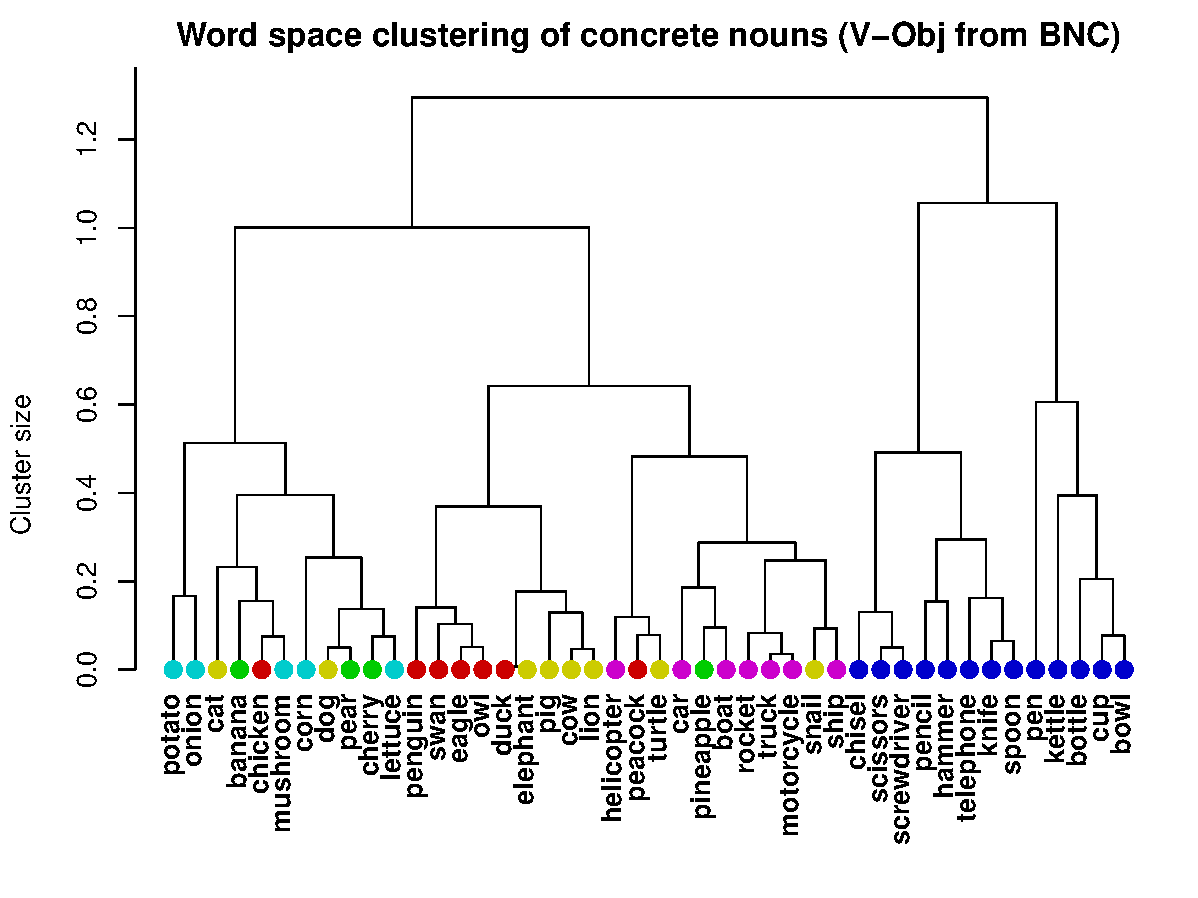
\includegraphics[width=8cm]{img/hieroglyph_clustering}}%
  \only<beamer:2-| handout:1>{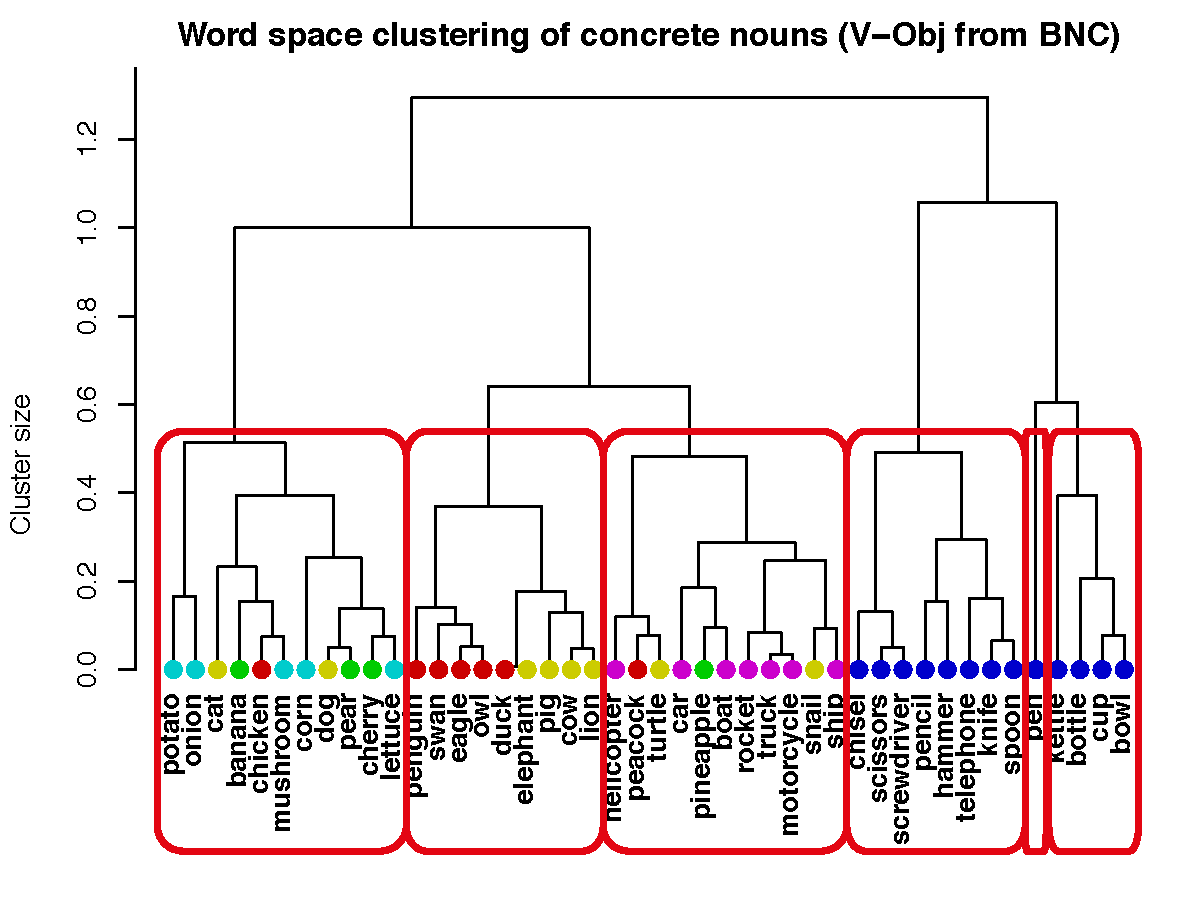
\includegraphics[width=8cm]{img/hieroglyph_clustering_6}}%
\end{center}
\ungap[1]
\begin{itemize}
\item<3-> majority labels: greens, birds, vehicles, tools, tools, tools
\item<3-> correct: 5/11, 5/9, 7/11, 8/8, 1/1, 4/4
\item<4-> purity = 30 correct out of 44 = 68.2\%
\end{itemize}
\end{frame}

\begin{frame}
\frametitle{ESSLLI 2008 shared task}
\begin{itemize}
\item Clustering experiments with CLUTO (Karypis 2003)
\begin{itemize}
\item repeated bisection algorithm
\item 6-way (birds, ground animals, fruits, greens,
tools and vehicles), 3-way (animals, plants and
artifacts) and 2-way (natural and artificial entities) clusterings
\end{itemize}
\pause
\item Quantitative evaluation
\begin{itemize}
\item \primary{entropy} -- whether words from different classes are represented in the same cluster (\secondary{best = 0})
\item \primary{purity} -- degree to which a cluster contains words from one class only (\secondary{best = 1})
\item \primary{global score} across the three clustering experiments
\begin{displaymath}
\sum_{i=1}^3 \text{Purity}_i -  \sum_{i=1}^3 \text{Entropy}_i
\end{displaymath}

\end{itemize}
\end{itemize}
\end{frame}

\frame{
\frametitle{ESSLLI 2008 shared task}

 \begin{center}
  \begin{tabular}{|l|r|r||r|r||r|r||r|}
      \hline
      \emph{model} &\multicolumn{2}{|c||}{\emph{6-way}} &  \multicolumn{2}{|c||}{\emph{3-way}} & \multicolumn{2}{|c||}{\emph{2-way}}&  \multicolumn{1}{|c|}{\emph{global}}\\
      \cline{2-7}
      &   \emph{P} & \emph{E}  & \emph{P} & \emph{E}  & \emph{P} & \emph{E} &\\
      \hline
      \hline
      Katrenko & 89 & 13 & 100 & 0 & 80 & 59 & 197\\ 
      \hline
      Peirsman+ & 82 & 23 & 84 & 34 & 86 & 55 & 140\\
      \hline
      dep-typed (DM) & 77 & 24 & 79 & 38 & 59 & 97 & 56\\
      \hline
      dep-filtered (DM) & 80 &28 & 75& 51& 61& 95 & 42\\
      \hline
      window (DM) & 75& 27&  68& 51& 68& 89   &44\\
      \hline
      Peirsman$-$ & 73 & 28 & 71 & 54 & 61 & 96 & 27\\
      \hline
      Shaoul & 41& 77& 52& 84 & 55& 93& -106\\
      \hline
    \end{tabular}
\end{center}

\begin{center}\footnotesize
  {\tt Katrenko, Peirsman+/-, Shaoul}: ESSLLI 2008 Shared Task\\
  {\tt DM}: Baroni \& Lenci (2009)
\end{center}

}

\begin{frame}
  \frametitle{Semantic priming}
  \begin{itemize}
  \item Hearing/reading a ``related'' prime facilitates access to a
    target in various lexical tasks (naming, lexical decision,
    reading)
    \begin{itemize}
  \item the word \emph{pear} is recognized faster if heard/read after \emph{apple}
  \item[]
    \end{itemize}
  \item<2-> \citet{Hodgson:91} single word lexical decision task, 136
    prime-target pairs \citep[cf.][]{Pado:Lapata:07}
    \begin{itemize}
  \item similar amounts of priming found for different  semantic relations between primes and targets ($\approx 23$ pairs
    per relation)
    \begin{itemize}
    \item synonyms (synonym): \emph{to dread/to fear}
    \item antonyms (antonym): \emph{short/tall}
    \item coordinates (coord): \emph{train/truck}
    \item super- and subordinate pairs (supersub): \emph{container/bottle}
    \item free association pairs (freeass): \emph{dove/peace}
    \item phrasal associates (phrasacc): \emph{vacant/building}
    \end{itemize}
  \end{itemize}
\end{itemize}
\end{frame}



\begin{frame}
  \frametitle{Simulating semantic priming}
  \framesubtitle{\citet{McDonald:Brew:04,Pado:Lapata:07}}
 \begin{itemize}
 \item DSMs and semantic priming
  \begin{enumerate}
  \item for each related prime-target pair, 
  measure cosine-based similarity between items (e.g.,
    \emph{to dread / to fear})
    \pause
  \item to estimate \primary{unrelated primes}, take average of cosine-based similarity of target with other primes from same semantic relation (e.g., \emph{value / to fear})
    \pause
  \item similarity between related items should be significantly higher
    than average similarity between unrelated items
    \item[]
  \end{enumerate}
\item<2-> Significant effects ($p < .01$) for all semantic relations 
  \begin{itemize}
  \item strongest effects for synonyms, antonyms \& coordinates
  \item[]
  \end{itemize}
\item<3-> Alternative: \primary{classification} task
  \begin{itemize}
  \item given target and two primes, identify related prime\\ (\so multiple choice like TOEFL)
  \end{itemize}
  \end{itemize}
\end{frame}


%%%%%%%%%%%%%%%%%%%%%%%%%%%%%%%%%%%%%%%%%%%%%%%%%%%%%%%%%%%%%%%%%%%%%% 
\section{Parameter evaluation}

%%%%%%%%%%%%%%%%%%%%%%%%%%%%%%%%%%%%%%%%%%
\subsection{Evaluation strategies}

\begin{frame}
  \frametitle{DSM evaluation in published studies}

  \begin{itemize}
  \item \primary{One model, many tasks} \citep{Pado:Lapata:07,Baroni:Lenci:10}
    \begin{itemize}
    \item A novel DSM is proposed, with specific features \& parameters
    \item This DSM is tested on a range of different tasks (e.g.\ TOEFL, priming, semantic clustering)
    \item[]
    \end{itemize}

  \item<2-> \primary{Incremental tuning of parameters} \citep{Bullinaria:Levy:07,Bullinaria:Levy:12,Kiela:Clark:14,Polajnar:Clark:14}
    \begin{itemize}
    \item Several parameters (e.g., scoring measure, distance metric, dimensionality reduction) 
    \item Many tasks (e.g.\ TOEFL, semantic \& syntactic clustering)
    \item Varying granularity of parameter settings
    \item One parameter (sometimes two) varied at a time, with all other parameters set to fixed values or optimized for each setting
    \item Optimal parameter values are determined sequentially
    \end{itemize}

  \end{itemize}
\end{frame}



%%%%%%%%%%%%%%%%%%%%%%%%%%%%%%%%%%%%%%%%%%
\subsection{An example (Bullinaria \& Levy 2007, 2012)}

\begin{frame}
  \frametitle{Bullinaria \& Levy (2007, 2012)}

  \ungap[1]
  \begin{itemize}
  \item One of the first systematic evaluation studies
  \item Test influence of many standard parameter settings
    \begin{itemize}
    \item frequency weighting + distance measure
    \item co-occurrence window, structured \vs unstructured
    \item corpus type \& size, number of feature dimensions
    \item dimensionality reduction (SVD), number of latent dimension
    \end{itemize}
  \item<2-> In four different evaluation tasks
    \begin{itemize}
    \item TOEFL
    \item distance comparison: related word \vs 10 random words
    \item semantic categorization: nearest-centroid classifier
    \item syntactic categorization (2007)
    \item semantic clustering of nouns (2012)
    \end{itemize}
  \item<3-> Novel parameters
    \begin{itemize}
    \item skipping of first latent dimensions (with highest variance)
    \item Caron's (\citeyear{Caron:01}) $P$: power-scaling of singular values
    \end{itemize}
  \end{itemize}
\addnote{Note that B\&L do not test all commonly used parameter settings, e.g.\ log-likelihood or log frequency as feature weighting.}%
\addnote{They also do not seem to normalize row vectors properly (frequency vectors are scaled to probabilities, i.e.\ $\norm[1]{x} = 1$), which might explain the poor results from Euclidean distance.}%
\addnote{Noun clustering uses \citet{Mitchell:etc:08} dataset of 60 nouns from 12 categories, and CLUTO direct clustering with standard settings.}%
\addnote{Incremental approach also across the two studies: B\&L (2012) builds on and extends results of B\&L (2007).}%
\addnote{Note that B\&L's power scaling notation differs from \citet{Caron:01}: $P = 1 + p/2$}%
\end{frame}

\begin{frame}
  \frametitle{TOEFL results: feature weighting \& distance measure}
  \framesubtitle{\citep[p.~516, Fig.~1]{Bullinaria:Levy:07}}

  \ungap[1.5]
  \begin{center}
    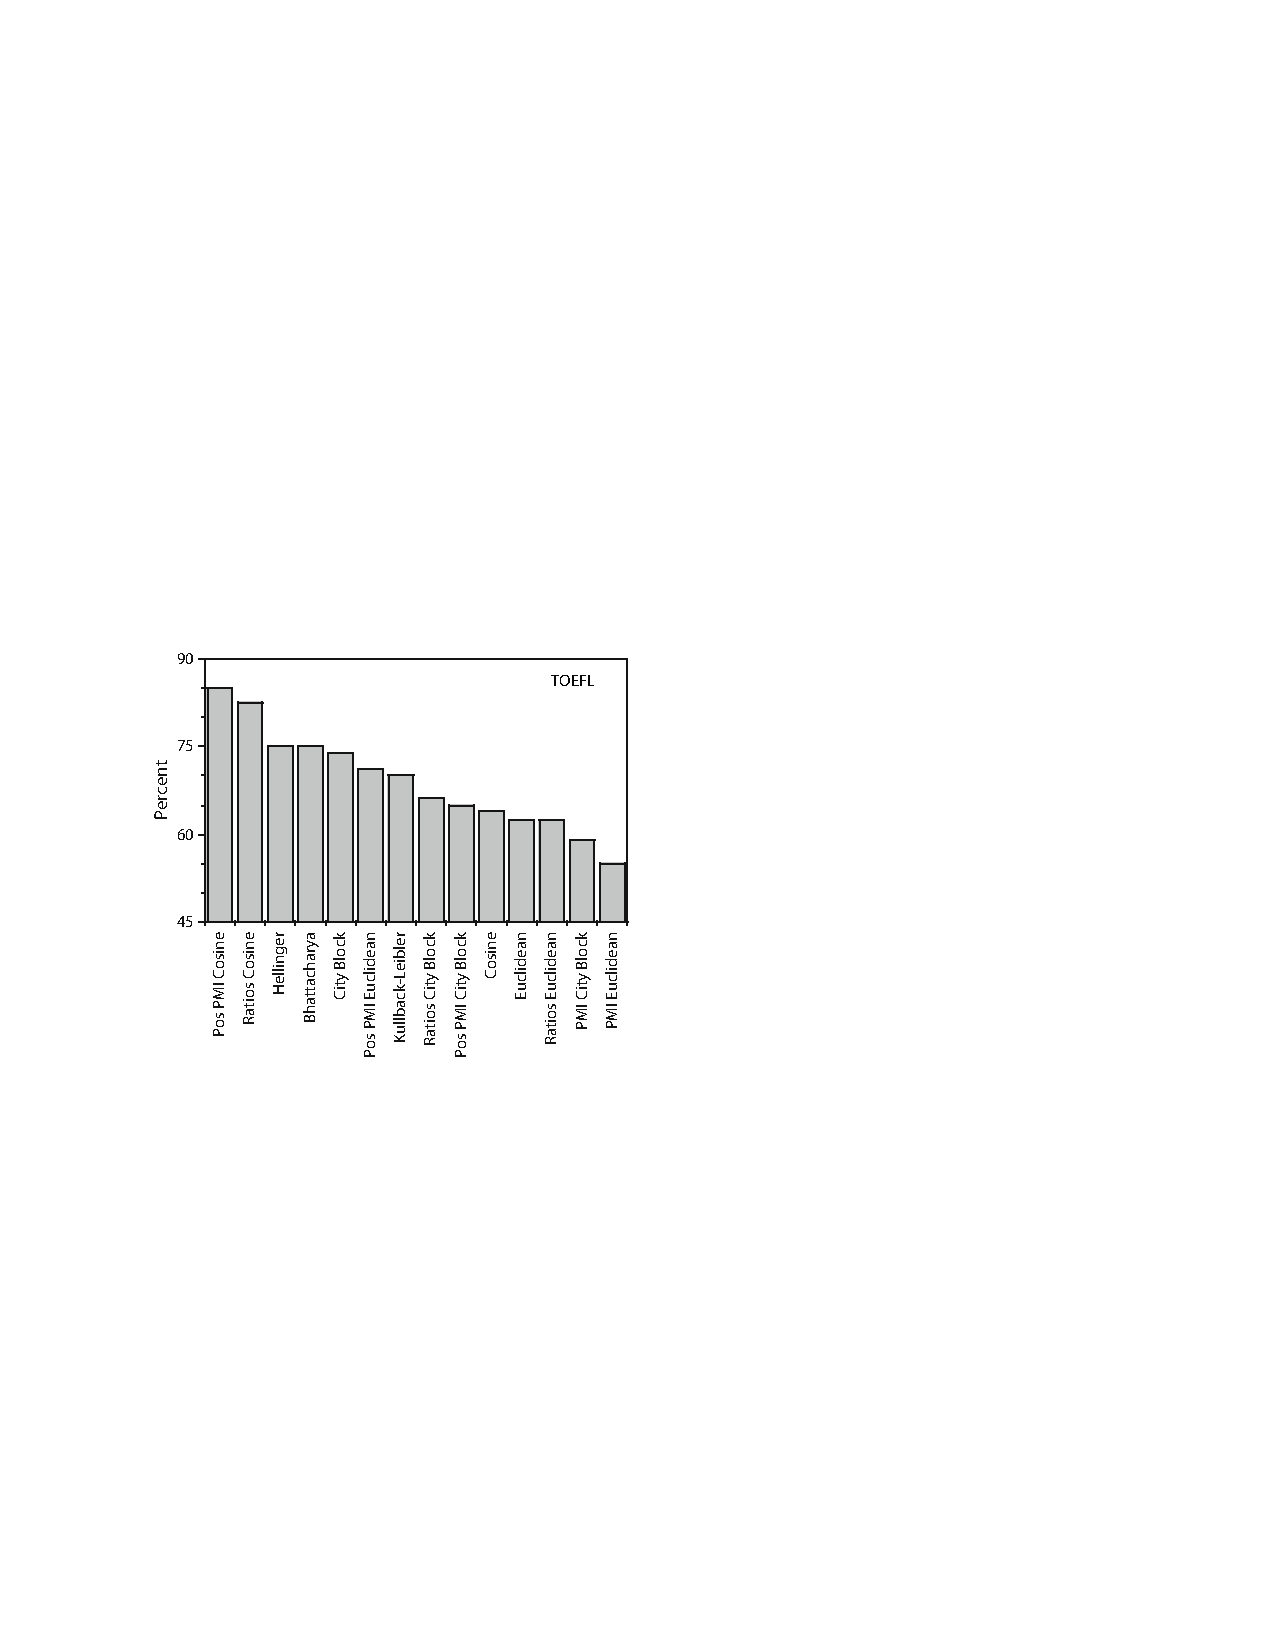
\includegraphics[width=7cm]{img/BullinariaLevy2007_p516_fig1_TOEFL_metric}
  \end{center}

  \ungap[1]
  \secondary{\scriptsize
   British National Corpus (BNC). Vectors not L2-normalized (frequency is L1-normalized). All other parameters optimized for each setting.
    \par% terminate paragraph to recompute line spacing while \scriptsize is still in effect
  }
\end{frame}

\begin{frame}
  \frametitle{TOEFL results: size \& type of co-occurrence window}
  \framesubtitle{\citep[p.~893, Fig.~1]{Bullinaria:Levy:12}}

  \ungap[1]
  \begin{center}
    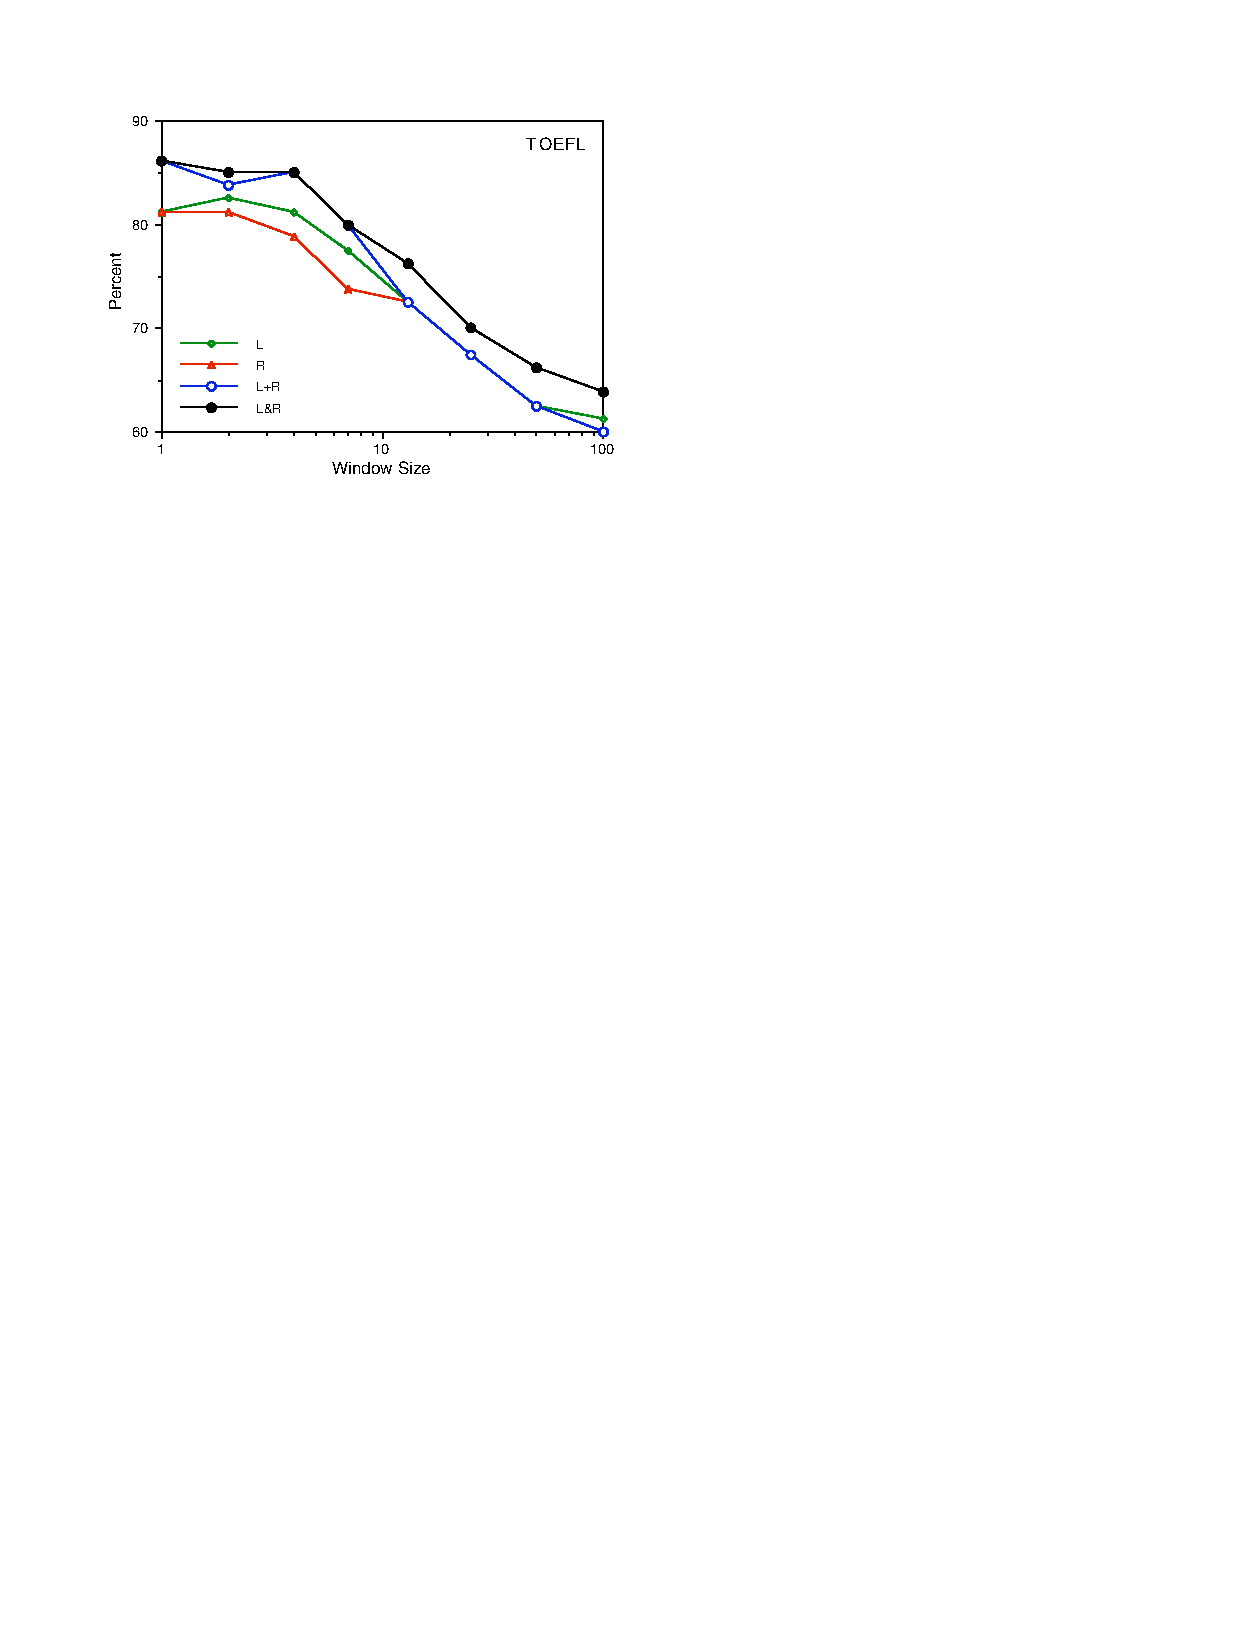
\includegraphics[width=8cm]{img/BullinariaLevy2012_p893_fig1_TOEFL_window}
  \end{center}

  \ungap[.5]
  \secondary{\scriptsize
    ukWaC Web corpus. Positive PMI + cosine \citep{Bullinaria:Levy:07}. Number of feature dimensions optimized for each window size \& task. No dimensionality reduction. L\&R = structured surface context (left/right).
    \par%
  }
\end{frame}

\begin{frame}
  \frametitle{TOEFL results: corpus type \& size}
  \framesubtitle{\citep[p.~894, Fig.~2]{Bullinaria:Levy:12}}

  \ungap[1]
  \begin{center}
    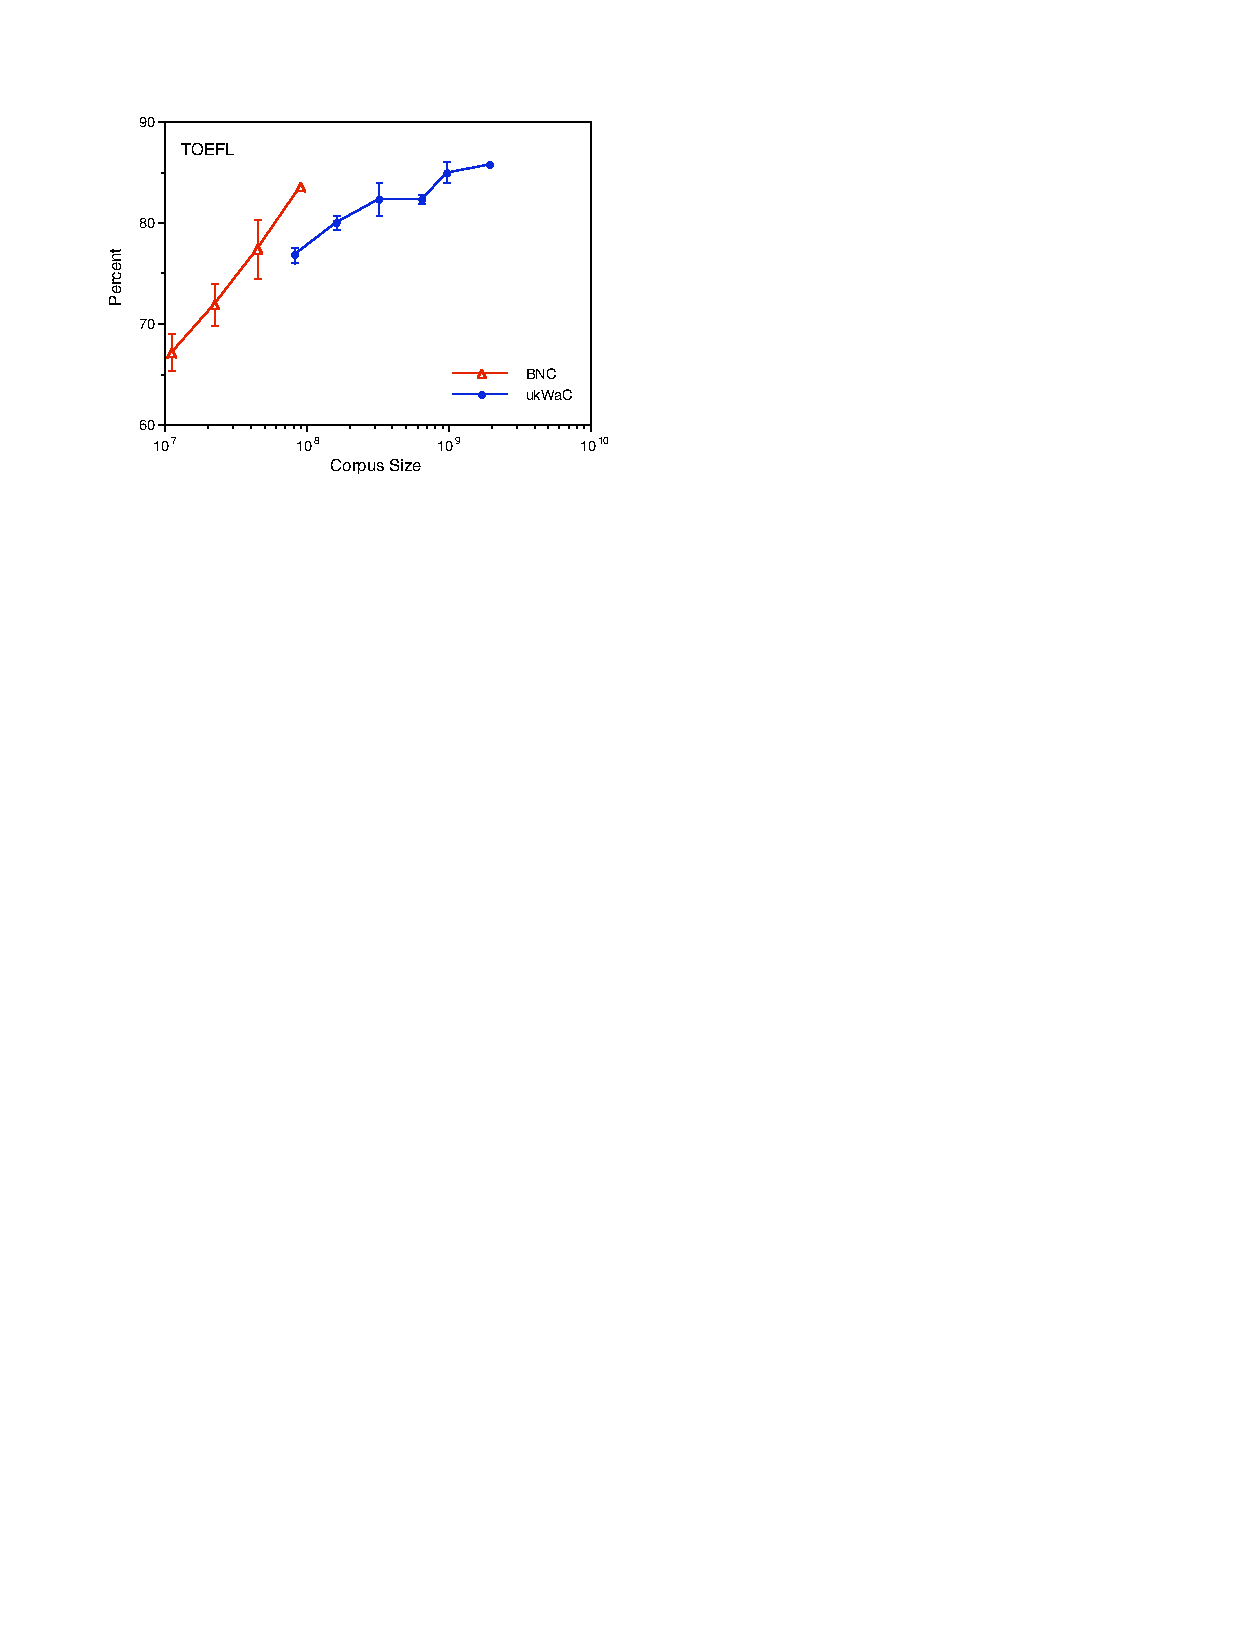
\includegraphics[width=8cm]{img/BullinariaLevy2012_p894_fig2_TOEFL_size}
  \end{center}

  \ungap[.5]
  \secondary{\scriptsize
    L+R context of size 1. Average + standard error over equally-sized corpus slices. Other parameter settings unclear.
    \par%
  }
\end{frame}

\begin{frame}
  \frametitle{TOEFL results: feature dimensions \& pre-processing}
  \framesubtitle{\citep[p.~895, Fig.~4]{Bullinaria:Levy:12}}

  \ungap[1]
  \begin{center}
    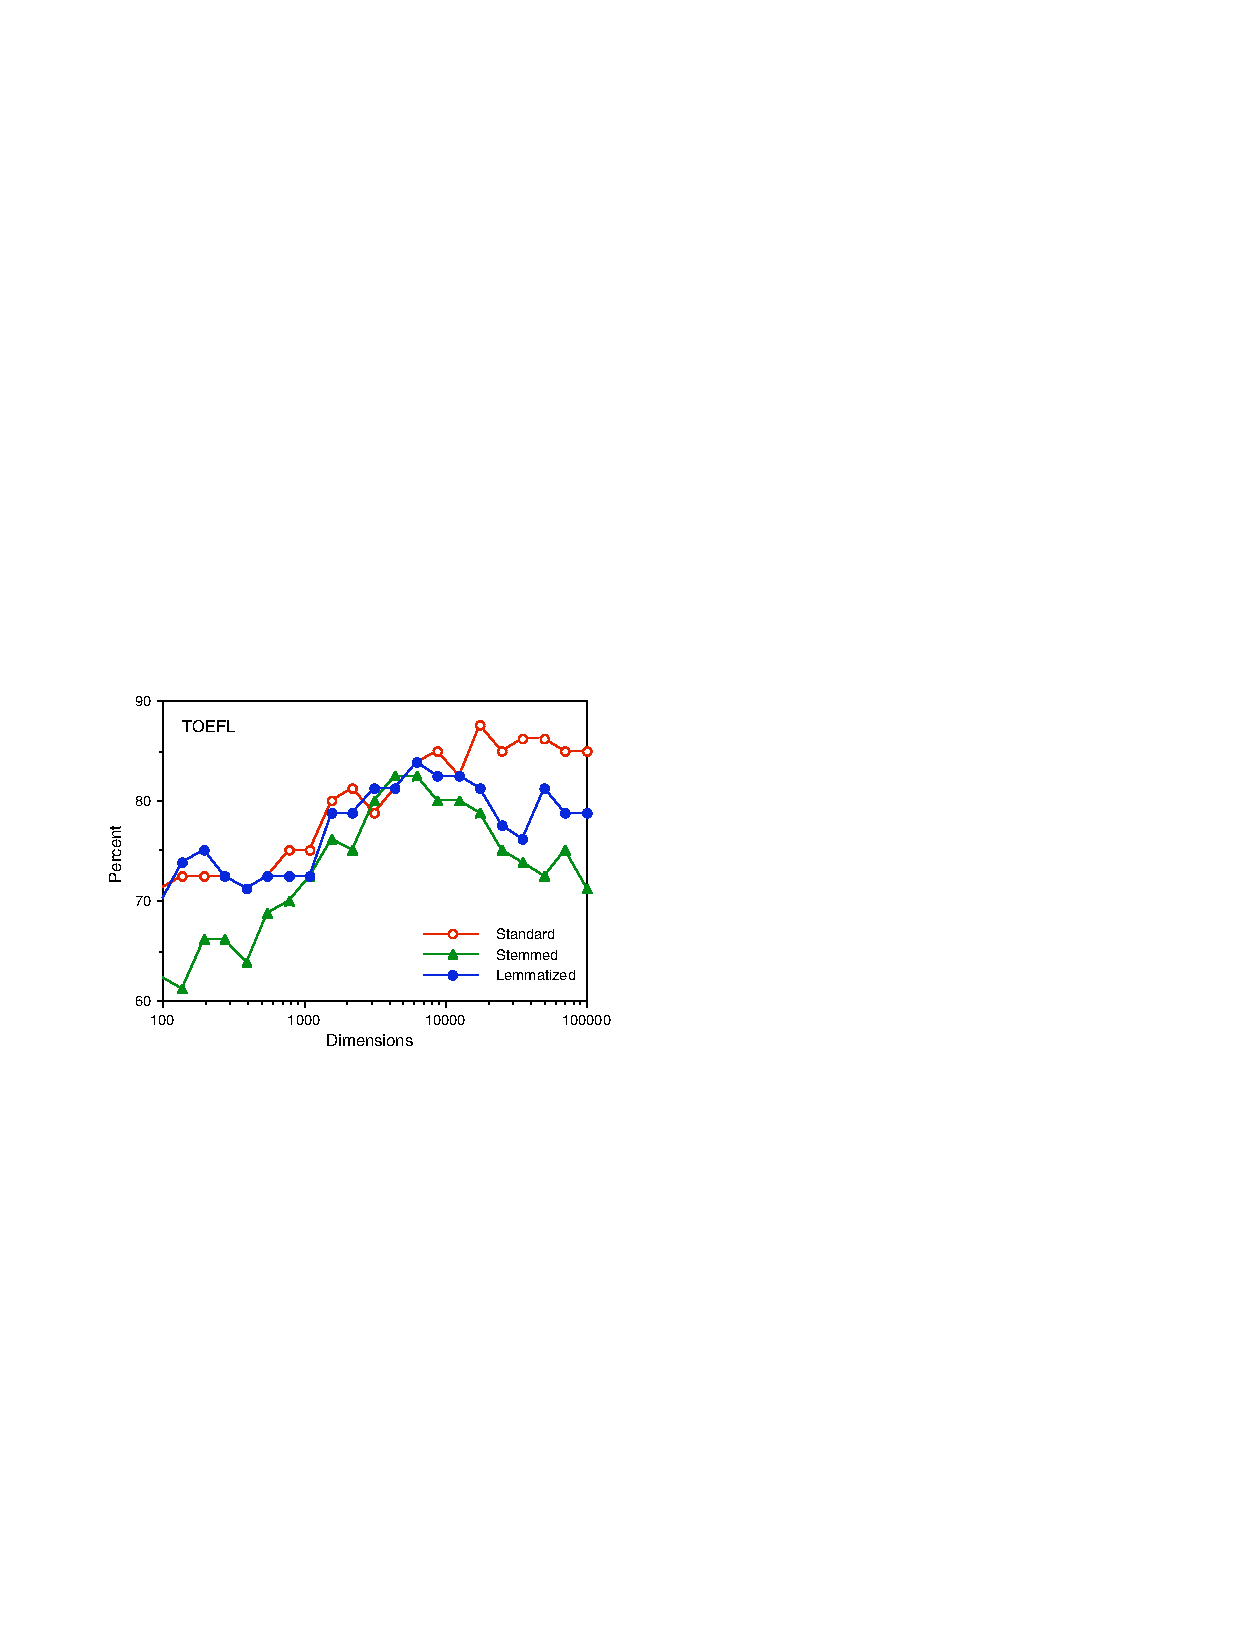
\includegraphics[width=8cm]{img/BullinariaLevy2012_p895_fig4_TOEFL_dim_stem}
  \end{center}

  \ungap[.5]
  \secondary{\scriptsize
    ukWaC corpus. L+R context of size 1. Other parameters presumably as above.
    \par%
  }
\end{frame}

\begin{frame}
  \frametitle{TOEFL results: dimensionality reduction}
  \framesubtitle{\citep[p.~898, Fig.~5]{Bullinaria:Levy:12}}

  \ungap[1]
  \begin{center}
    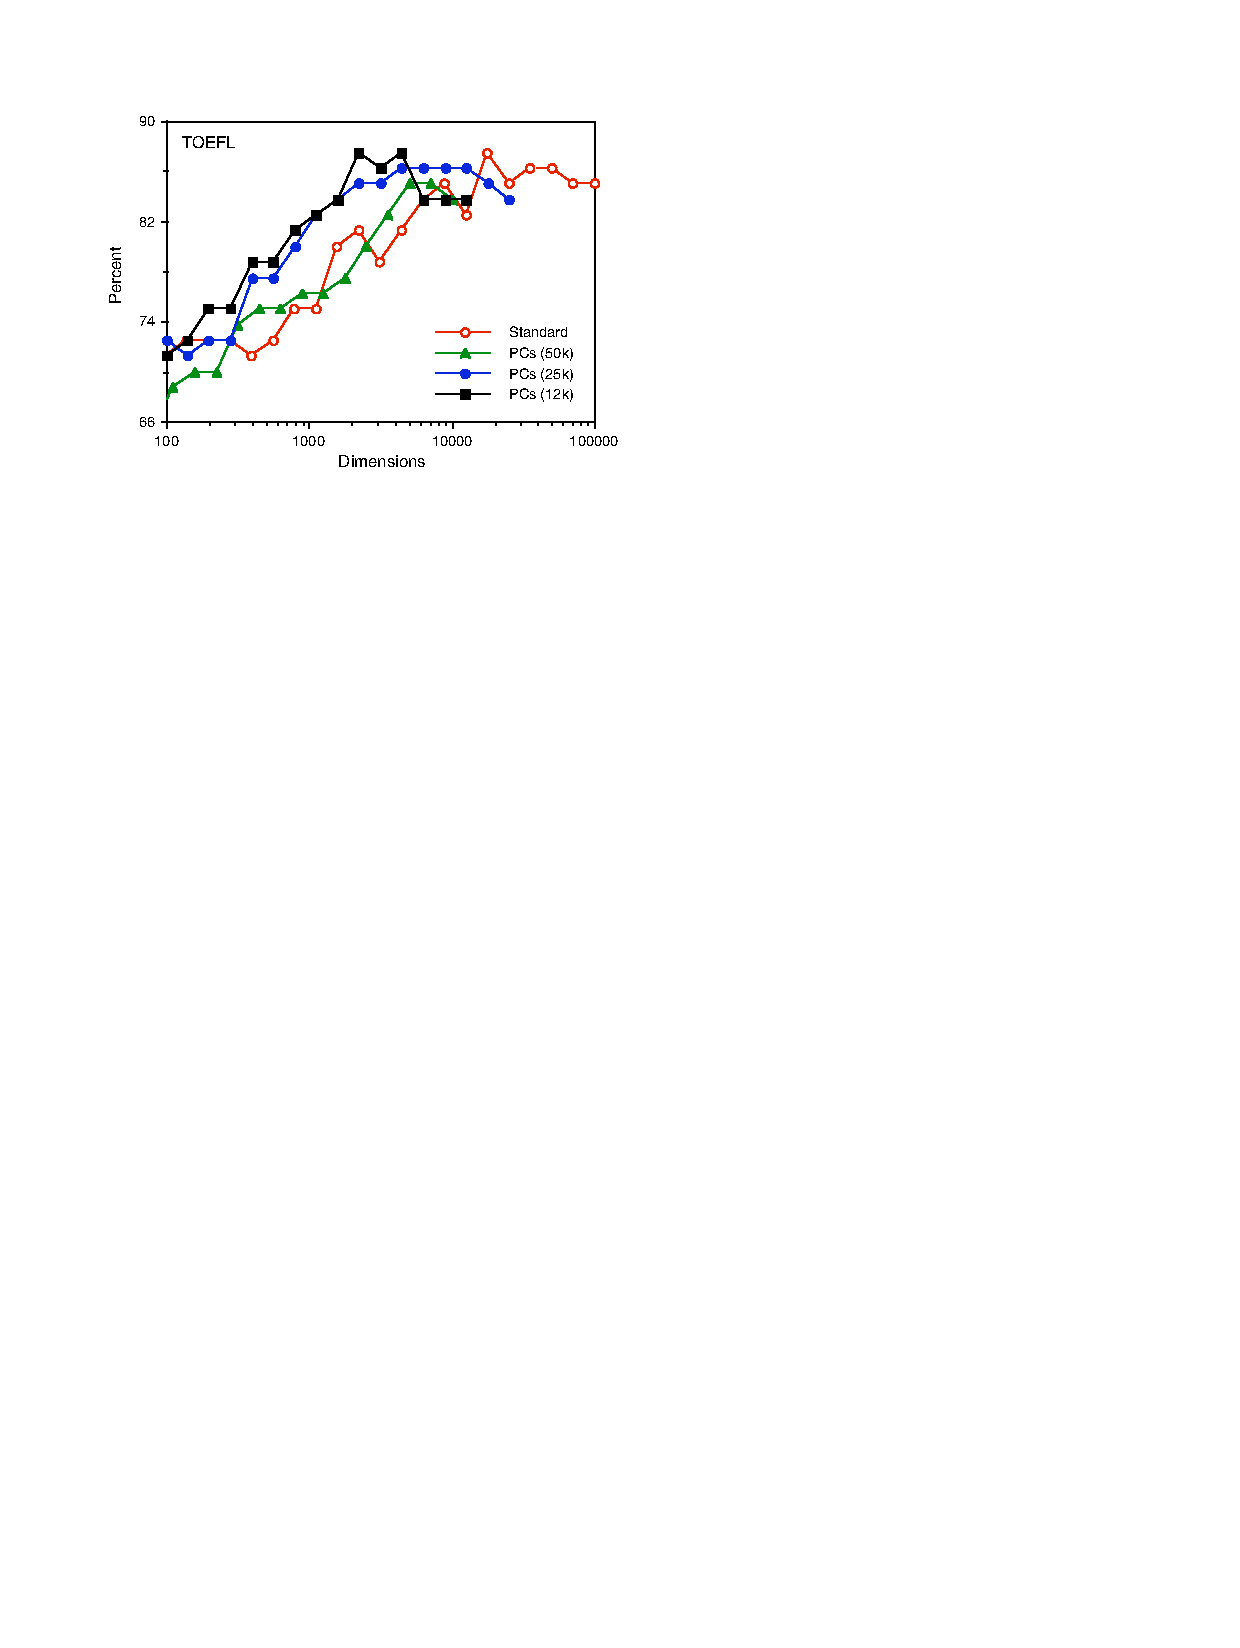
\includegraphics[width=8cm]{img/BullinariaLevy2012_p898_fig5_TOEFL_reddim}
  \end{center}

  \ungap[.5]
  \secondary{\scriptsize
    ukWaC corpus. Positive PMI + cosine. Standard = no dimensionality reduction.
    Other: number of latent dimensions for 12k, 25k and 50k original feature dimensions.
    \par%
  }
\end{frame}

\begin{frame}
  \frametitle{Semantic Categorization: dimensionality reduction}
  \framesubtitle{\citep[p.~898, Fig.~5]{Bullinaria:Levy:12}}

  \ungap[1]
  \begin{center}
    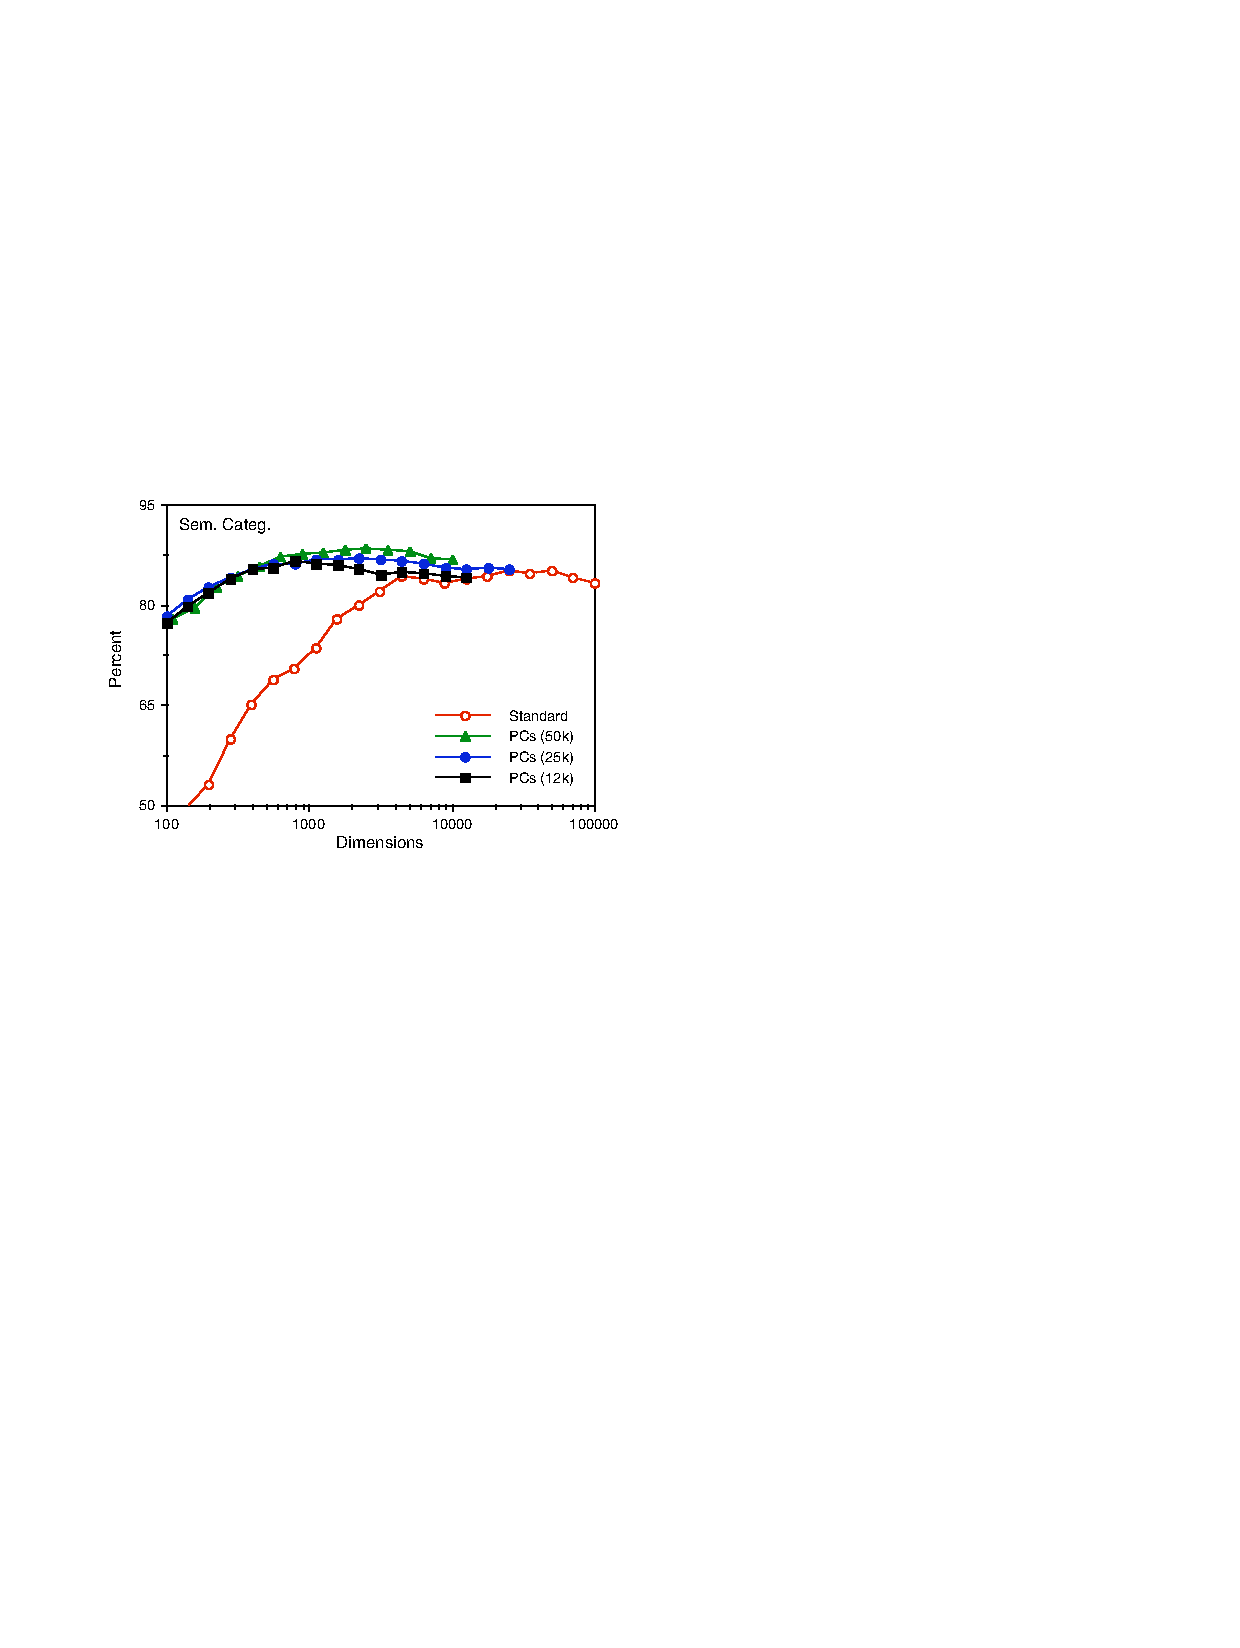
\includegraphics[width=8cm]{img/BullinariaLevy2012_p898_fig5_SemCat_reddim}
  \end{center}

  \ungap[.5]
  \secondary{\scriptsize
    ukWaC corpus. Positive PMI + cosine. Standard = no dimensionality reduction.
    Other: number of latent dimensions for 12k, 25k and 50k original feature dimensions.
    \par%
  }
\end{frame}

\begin{frame}
  \frametitle{Combined results: skipping first latent dimensions}
  \framesubtitle{\citep[p.~900, Fig.~7]{Bullinaria:Levy:12}}

  \ungap[1.5]
  \begin{center}
    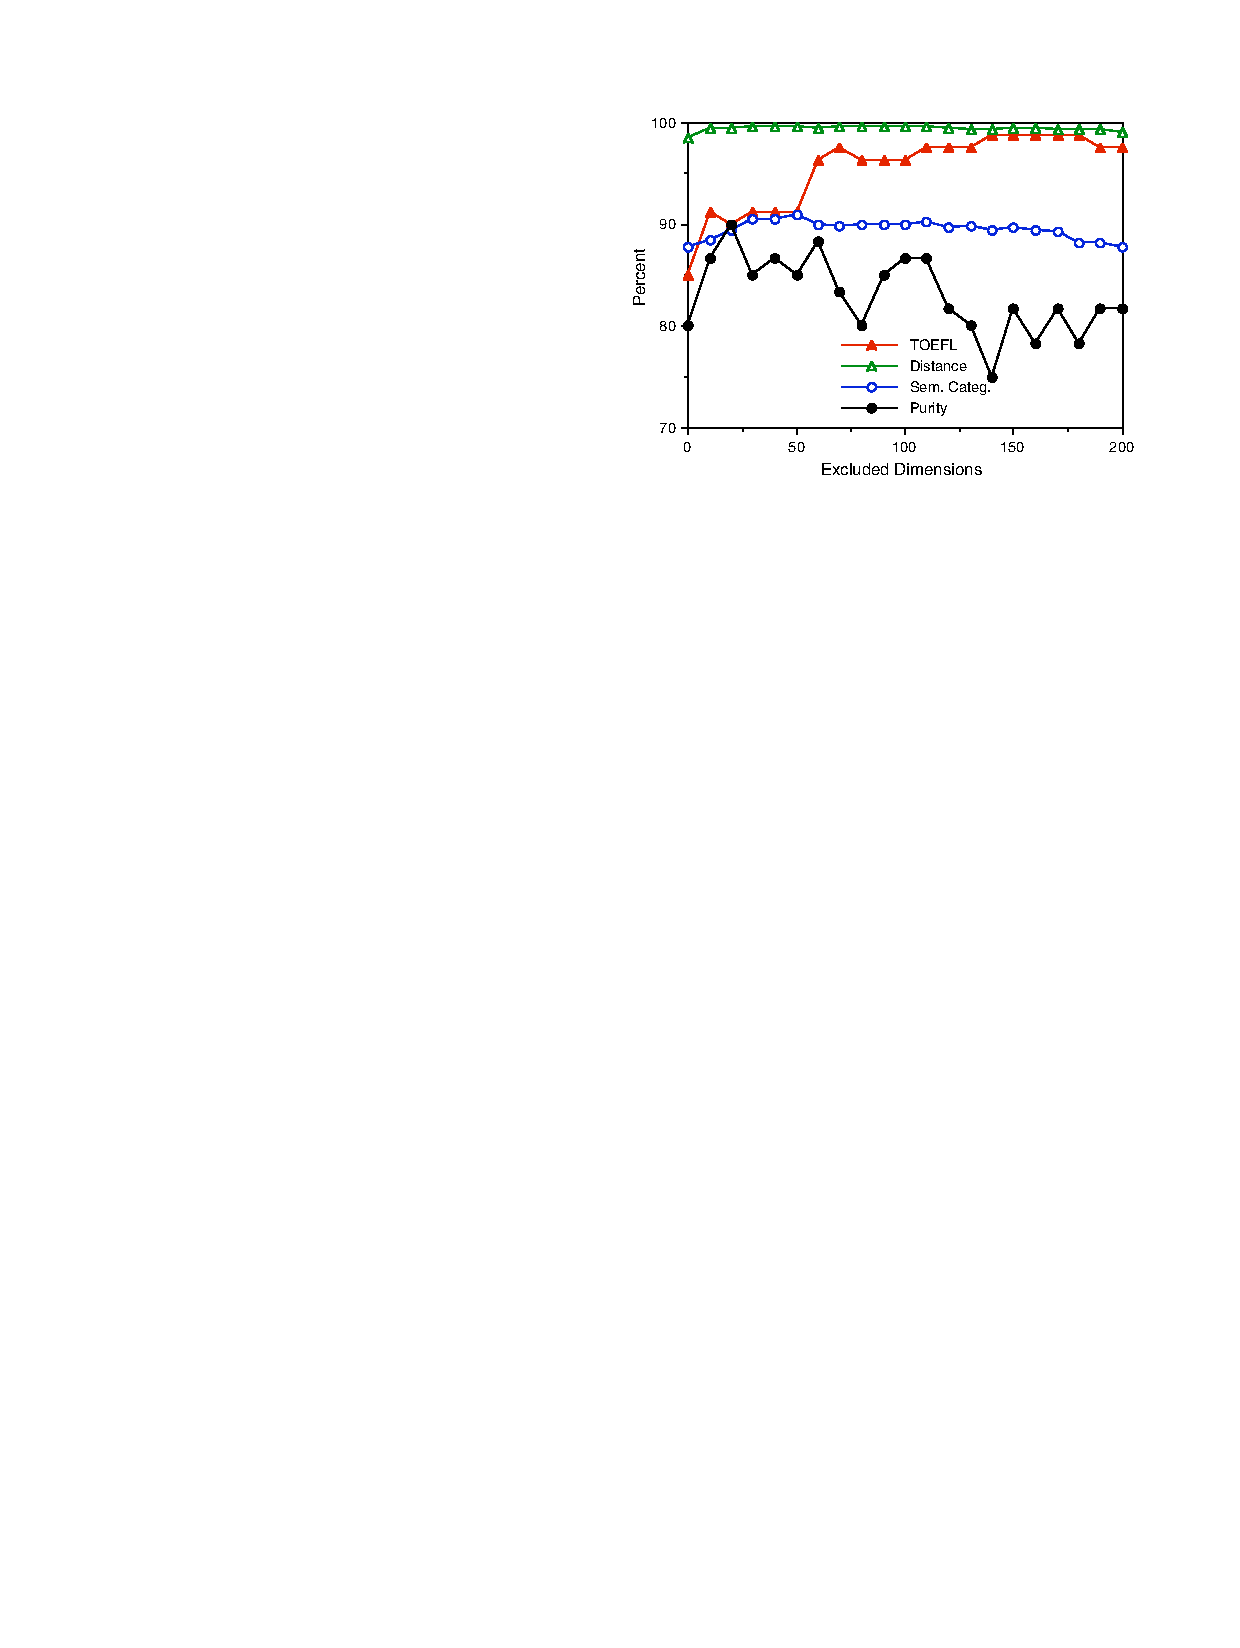
\includegraphics[width=8cm]{img/BullinariaLevy2012_p900_fig7_skipdim}
  \end{center}

  \ungap[.5]
  \secondary{\scriptsize
    ukWaC corpus with standard settings. 50k feature dimensions reduced to 5000 latent dimensions.
    \par%
  }
\end{frame}

\begin{frame}
  \frametitle{TOEFL results: power scaling (Caron's $P$)}
  \framesubtitle{\citep[p.~900, Fig.~7]{Bullinaria:Levy:12}}

  \ungap[1.5]
  \begin{center}
    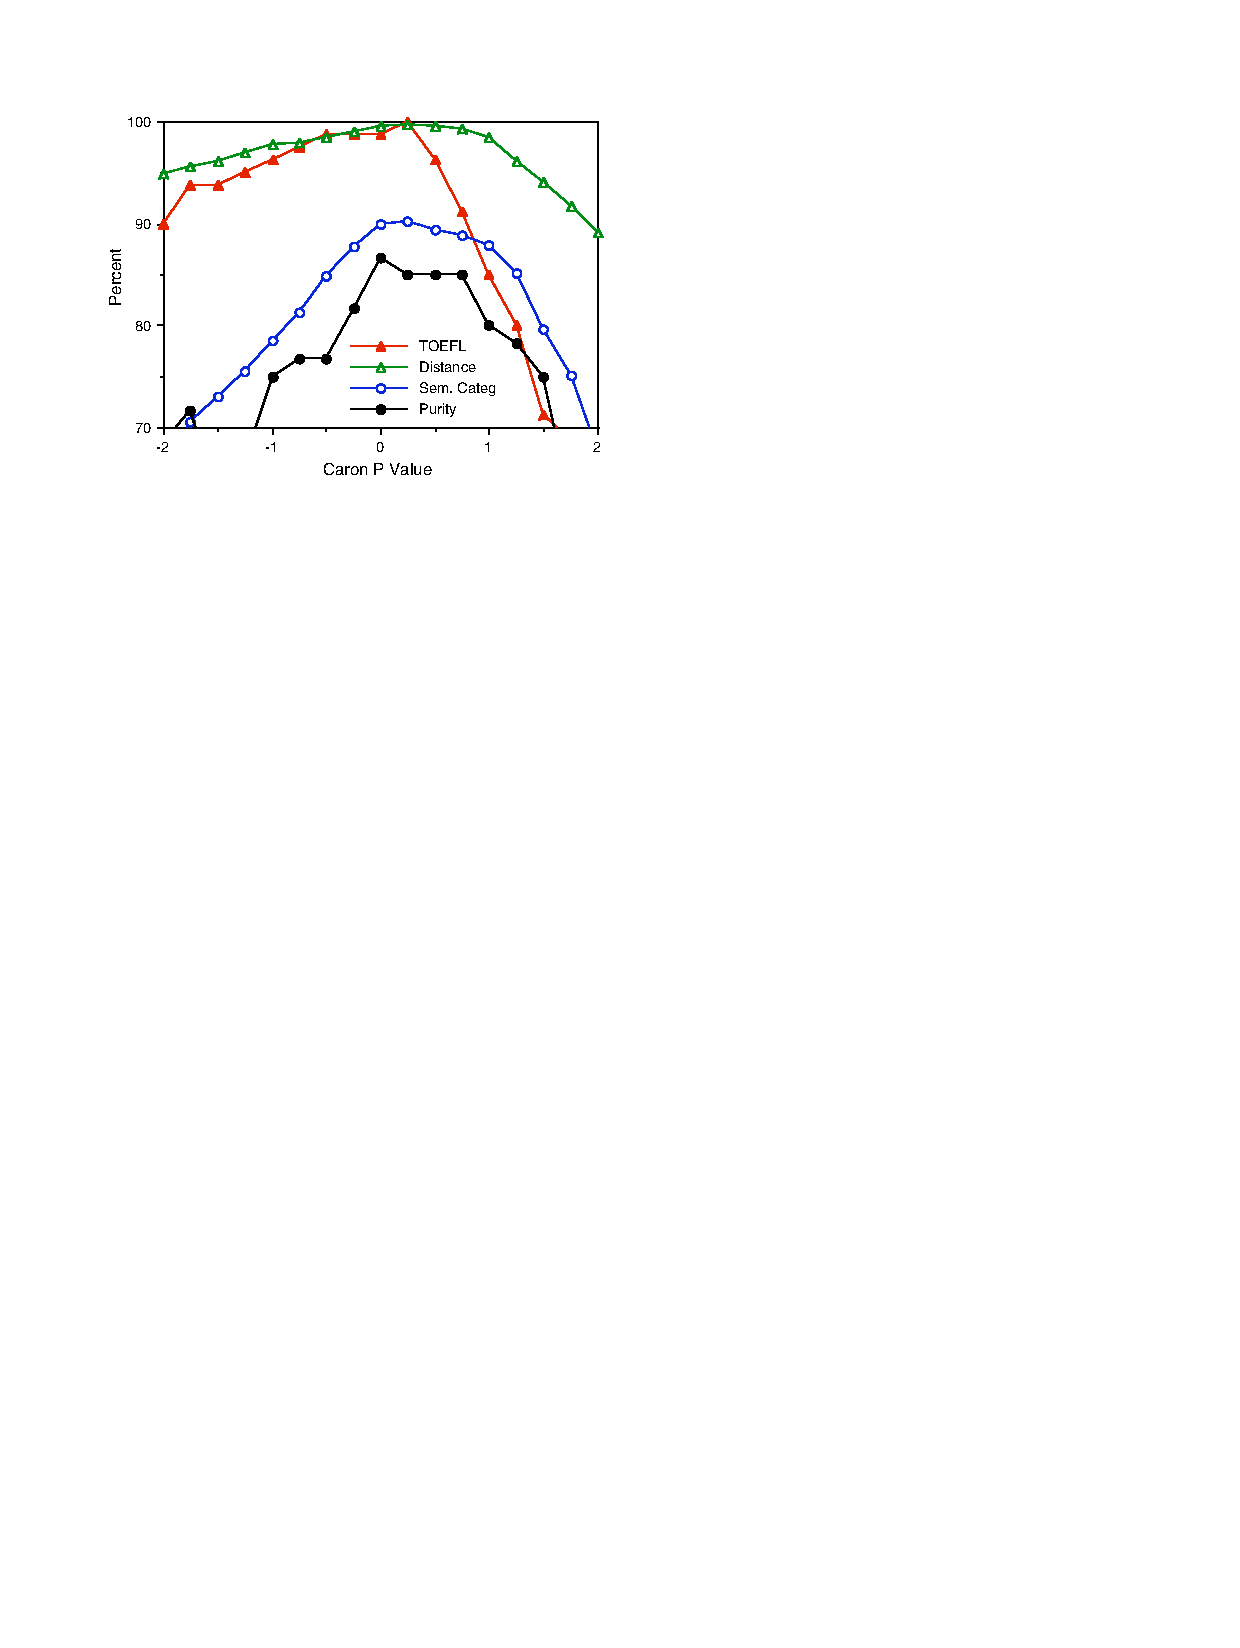
\includegraphics[width=8cm]{img/BullinariaLevy2012_p900_fig7_power}
  \end{center}

  \ungap[.5]
  \secondary{\scriptsize
    ukWaC corpus with standard settings. 50k feature dimensions reduced to 5000 latent dimensions.
    Neutral value is $P = 1$.
    \par%
  }
\end{frame}



%%%%%%%%%%%%%%%%%%%%%%%%%%%%%%%%%%%%%%%%%%%%%%%%%%%%%%%%%%%%%%%%%%%%%%
\section{A large scale evaluation study}

\begin{frame}[c]
  \centering

  \hh{\large A (very) large-scale evaluation study}
  
  \gap[2]
  Based on research by Gabriella Lapesa.
\end{frame}

%%%%%%%%%%%%%%%%%%%%%%%%%%%%%%%%%%%%%%%%%%
\subsection{Tasks \& parameters}

\begin{frame}
  \frametitle{Tasks}

  \begin{enumerate}
  \item \hh{Classification}
    \begin{itemize}
    \item TOEFL multiple-choice classification task \citep{Landauer:Dumais:97}
    \item[]
    \end{itemize}
  \item \hh{Correlation to Similarity Ratings}
    \begin{itemize}
    \item RG65: 65 noun pairs \citep{Rubenstein:Goodenough:65}
    \item WordSim353: 351 noun pairs \citep{Finkelstein:etc:02}
    \item[]
    \end{itemize}  
  \item \hh{Semantic Clustering} 
    \begin{itemize} 
    \item Battig: 83 nouns, 10 classes \citep{VanOverschelde:Rawson:Dunlosky:04}
    \item AP: 402 nouns, 21 classes \citep{Almuhareb:06}
    \item ESSLLI 2008: 44 nouns, 6 classes\footnote{\scriptsize\url{http://wordspace.collocations.de/doku.php/data:esslli2008:concrete_nouns_categorization}}
    \item Mitchell: 60 nouns, 12 classes \citep{Mitchell:etc:08}
    \item[]
    \end{itemize}   
  \end{enumerate}
\end{frame}

\begin{frame}
  \frametitle{Distributional models: general features}
  \begin{itemize}
  \item \primary{Term-term} distributional semantic models (bag-of-words)
  \item \secondary{Target} terms (rows)
    \begin{itemize}
    \item vocabulary from Distributional Memory \citep{Baroni:Lenci:10} + terms from evaluation datasets
    \item 27522 lemma types 
    \end{itemize} 
  \item \secondary{Feature} terms (columns)
    \begin{itemize}
    \item filtered by part-of-speech (nouns, verbs, adjectives, adverbs)
    \item further context selection determined by two model parameters
    \end{itemize}
  \end{itemize}

  \begin{block}{}\footnotesize
    Distributional models were compiled and evaluated using the IMS \primary{Corpus Workbench}\footnote{\scriptsize\url{http://cwb.sf.net/}}, the \primary{UCS toolkit}\footnote{\scriptsize\url{http://www.collocations.de/software.html}} and the \primary{\texttt{wordspace} package}\footnote{\scriptsize\url{http://wordspace.r-forge.r-project.org/}} for R.
  \end{block}

\end{frame}

\begin{frame}
  \frametitle{Evaluated parameters}
  \framesubtitle{Building the co-occurrence matrix}
  \begin{enumerate}
  \item   \h{Source corpus}: BNC, Wackypedia, UkWac
    \begin{block}{}\small
      Our source corpora -- standard choices in distributional semantics -- differ in both size and quality. Is there a quantity/quality trade-off?
    \end{block}
    
  \item  \textbf{Window}
    \begin{itemize}
    \item  \h{Direction}: directed (= structured), undirected
    \item  \h{Size}: 1, 2, 4, 8, 16 words
    \end{itemize}   
    
    \begin{block}{}\small
      We expect those parameters to be crucial as they determine the granularity (direction) and amount (size) of shared context involved in the computation of similarity.  
    \end{block}          
  \end{enumerate}   
\end{frame}

\begin{frame}
  \frametitle{Evaluated parameters}
  \framesubtitle{Selecting dimensions from the co-occurrence matrix} 
  \begin{enumerate}
    \setcounter{enumi}{2} 
  \item \textbf{Feature selection}: 
    \begin{itemize}
    \item   \h{Criterion}: frequency, number of non-zero entries 
    \item   \h{Threshold}: top $n$ dimensions ($n$ = 5000, 10000, 20000, 50000, 100000)
    \end{itemize}          
    \begin{block}{}\small
      How many context dimensions (words) are needed for DSMs to perform well in specific tasks? Are too many context dimensions detrimental? What is the best selection criterion? 
    \end{block}   
  \end{enumerate}   
\end{frame}


\begin{frame}
  \frametitle{Evaluated parameters}
  \framesubtitle{Weighting and scaling co-occurrence counts} 
  
  \begin{enumerate}
    \setcounter{enumi}{3}
    
  \item   \h{Feature scoring}: frequency, simple-ll, MI, Dice, t-score, z-score, tf.idf
    \begin{block}{}\small
      Association measures represent an interpretation of co-occurrence frequency, and they emphasize different types of collocations \citep{Evert:08}. Does this have an effect on DSM performance? 
    \end{block}
    
  \item  \h{Transformation}: none, logarithmic, square root, sigmoid
    \begin{block}{}\small
      Transformations reduce the skewness of feature scores.
    \end{block}
  \end{enumerate}   
\end{frame}

\begin{frame}
  \frametitle{Evaluated parameters}
  \framesubtitle{Dimensionality reduction}    

  \begin{enumerate}
    \setcounter{enumi}{5}
  \item \textbf{Dimensionality reduction} with randomized SVD:
    \begin{itemize}
    \item \h{number of reduced dimensions}: 100, 300, 500, 700, 900
    \item \h{number of skipped dimensions}: 0, 50, 100
    \end{itemize}    
    \begin{block}{}\small
      Dimensionality reduction is expected to improve semantic representation and make computations more efficient. How does SVD interact with the other parameters?
      \citet{Bullinaria:Levy:12} report improvements in some tasks (e.g.\ TOEFL) when the first latent dimensions (with highest variance) are discarded. Does this result generalize to our tasks/datasets? 
    \end{block}                  
  \end{enumerate}   
\end{frame}

\begin{frame}
  \frametitle{Evaluated parameters}
  \framesubtitle{Computation and usage of distances}   

  \begin{enumerate}
    \setcounter{enumi}{6}      
  \item   \h{Distance metric}: cosine (angular distance), manhattan
    \begin{block}{}\small
      Both are symmetric, while cognitive processes are often asymmetric
    \end{block}
    
  \item  \h{Index of distributional relatedness}
    \begin{itemize}
    \item \textbf{distance}: $\mathop{\text{dist}}(a,b)$
    \item  \textbf{neighbor rank}, calculated differently for different tasks:
      \begin{itemize}
      \item TOEFL: backward rank, i.e.\ $\mathop{\text{rank}}(b,a)$
      \item Ratings and Clustering: average of logarithmic forward and backward rank, i.e.\ $\bigl(\log \mathop{\text{rank}}(a,b) + \log \mathop{\text{rank}}(b,a)\bigr) / 2$
      \end{itemize}
    \end{itemize}    
    \begin{block}{}\small
      This parameter allows us to account for asymmetries: $\mathop{\text{rank}}(b,a)$ is different from $\mathop{\text{rank}}(a,b)$. While cognitively plausible, neighbor rank is computationally expensive: does it improve the performance of DSMs?
    \end{block}                
    
  \end{enumerate}   
\end{frame}

%%%%%%%%%%%%%%%%%%%%%%%%%%%%%%%%%%%%%%%%%%
\subsection{Methodology for DSM Evaluation}

\begin{frame}
  \frametitle{How many models did we end up with?}
  \framesubtitle{... and how do we make sense of all those results?}   

  \begin{itemize}
  \item We tested all the possible parameter combinations (we will see later that this is crucial for our evaluation methodology)
  \item \primary{537600 model runs} (33600 in the unreduced setting, 504000 in the reduced setting)
  \item The models were generated and evaluated on a large HPC cluster at FAU Erlangen-Nürnberg as well as servers at the University of Stuttgart, within approximately 5 weeks

  \end{itemize}
\end{frame}


\begin{frame}
  \frametitle{Evaluation methodology: linear regression}
  \framesubtitle{Our proposal for a robust evaluation of DSM parameters}

  \begin{itemize}
  \item Attempts to predict the values of a ``dependent'' variable from one or more ``independent'' variables and their combinations
  \item Is used to understand \secondary{which independent variables are closely related to the dependent variable}, and to \secondary{explore the forms of these relationships}
  \end{itemize}

  \begin{block}{Example}
    \textbf{Dependent variable}: income \\
    \textbf{Independent variables}: gender, age, ethnicity, education level, first letter of the surname \light{(hopefully not significant)}
  \end{block}



  
\end{frame}

\begin{frame}
  \frametitle{Evaluation methodology: linear regression}
  \framesubtitle{Our proposal for a robust evaluation of DSM parameters}

  We use linear models to analyze the influence of different DSM parameters and their combinations on DSM performance
  \begin{itemize}
  \item dependent variable = \primary{performance}\\
    (accuracy, correlation coefficient, purity)
  \item independent variables = model \primary{parameters}\\
    (e.g., source corpus, window size, window direction)
  \end{itemize}
  
  \begin{block}{}
    We want to understand which of the parameters are related to the dependent variable, i.e., we want to find the parameters whose manipulation has the strongest effect on DSM performance.
  \end{block}

\end{frame}


\begin{frame}
  \frametitle{DSM evaluation and linear regression}
  \framesubtitle{Toy example: a $2 \times 2 \times 2$ design}
  \centering
  \footnotesize
  \begin{tabular}{cccc}
    \hline
    Corpus & Window size &  Window direction &  Accuracy  \\  
    \hline 
    ukWaC & 1 & directed  &  88  \\  
    ukWaC & 16 & undirected   & 92 \\
    ukWaC & 1 & directed  &  91  \\  
    ukWaC & 16 & undirected   & 93 \\    
    BNC & 1  & undirected  &  80  \\  
    BNC & 16  & undirected  & 53   \\ 
    BNC & 1  & directed  &  72  \\  
    BNC & 16  & directed  & 71 \\   
    \hline
  \end{tabular}

  \begin{block}{}\small\ungap[2]
    \begin{align*}
      Accuracy &= \beta_{0} + \beta_1(\text{corpus})  + \beta_2(\text{window size}) +  \beta_3(\text{window direction}) \\
      & + \beta_4(\text{corpus: window size}) + \beta_5(\text{corpus: window direction}) + \\
      & + \beta_6(\text{window size: window direction})  + \epsilon
    \end{align*}
    \ungap[1.5]
  \end{block}
  
  \raggedright
  \light{\footnotesize *we're aware that this regression model is almost saturated \ldots}
\end{frame}

\begin{frame}
  \frametitle{DSM evaluation and linear regression}
  \framesubtitle{Analysis of variance}

  \begin{block}{}\footnotesize
    \primary{Goal}: quantify the impact of a specific parameter (or interaction) on DSM performance, in terms of the proportion of variance explained by the parameter
  \end{block}

  \footnotesize
  Key notions:
  \begin{itemize}
  \item \primary{$R^2$} (R squared)
    \begin{itemize}\footnotesize
    \item proportion of explained variance, i.e.\
      \[
      1 - \frac{\text{residual variance of $\epsilon$}}{\text{variance of dependent variable}}
      \]
    \item calculated (i) for the full model (\so how well the model exlains the experimental results) as well as (ii) for specific parameters and interactions (quantifying how much they contribute to predictions)
    \end{itemize}
  \item  \primary{Feature ablation}

  \end{itemize}
\end{frame}

\begin{frame}
  \frametitle{DSM evaluation and linear regression}
  \framesubtitle{Analysis of variance: feature ablation}

  \begin{block}{Feature ablation}
    Proportion of variance explained by a parameter together with all its interactions, corresponding to the reduction in  $R^2$ of the linear model fit if this parameter is left out. 
  \end{block}

  In our toy model with 3 parameters and all two-way interactions: 

  \begin{itemize}\footnotesize
  \item Ablation(corpus) $=$  $R^2$(corpus) +  $R^2$(corpus: window size) +  $R^2$(corpus: window direction)  
  \item Ablation(window size) $=$  $R^2$(window size) +  $R^2$(corpus: window size) +  $R^2$(window size: window direction)
  \item Ablation(window direction) $=$  $R^2$(window direction) +  $R^2$(corpus: window direction) +  $R^2$(window size: window direction) 
  \end{itemize}

\end{frame}

%%%%%%%%%%%%%%%%%%%%%%%%%%%%%%%%%%%%%%%%%%
\subsection{Evaluation on Standard Tasks}

\begin{frame}
  \frametitle{TOEFL multiple-choice classification task}
  \framesubtitle{Introducing the task}

  A collection of 80 multiple-choice questions from a synonym task in the Test Of English as a Foreign Language (TOEFL) 
  \begin{exampleblock}{TOEFL dataset}
    Target: \secondary{\emph{consume}} -- Choices: \emph{breed, catch, \primary{eat}, supply} \\
    Target: \secondary{\emph{constant}} -- Choices:  \emph{accidental, \primary{continuing}, instant, rapid}  \\
    Target: \secondary{\emph{concise}}\hspace{1ex} -- Choices: \emph{free, positive, powerful, \primary{succinct}} \\
  \end{exampleblock}
  \begin{itemize}
  \item A \textbf{classification} task
  \item If DSMs capture synonymy relations, we expect that \primary{the distance between the target and the correct choice will be smaller than to the wrong choices}
  \item Performance: \textbf{\% accuracy}
  \end{itemize}

  
\end{frame}

\begin{frame}
  \frametitle{TOEFL task: performance}
  \framesubtitle{Unreduced versus Reduced Experiments}
  \centering
  
  \begin{columns}

    \begin{column}{0.5\textwidth}
      \centering
      \hspace*{-18pt}   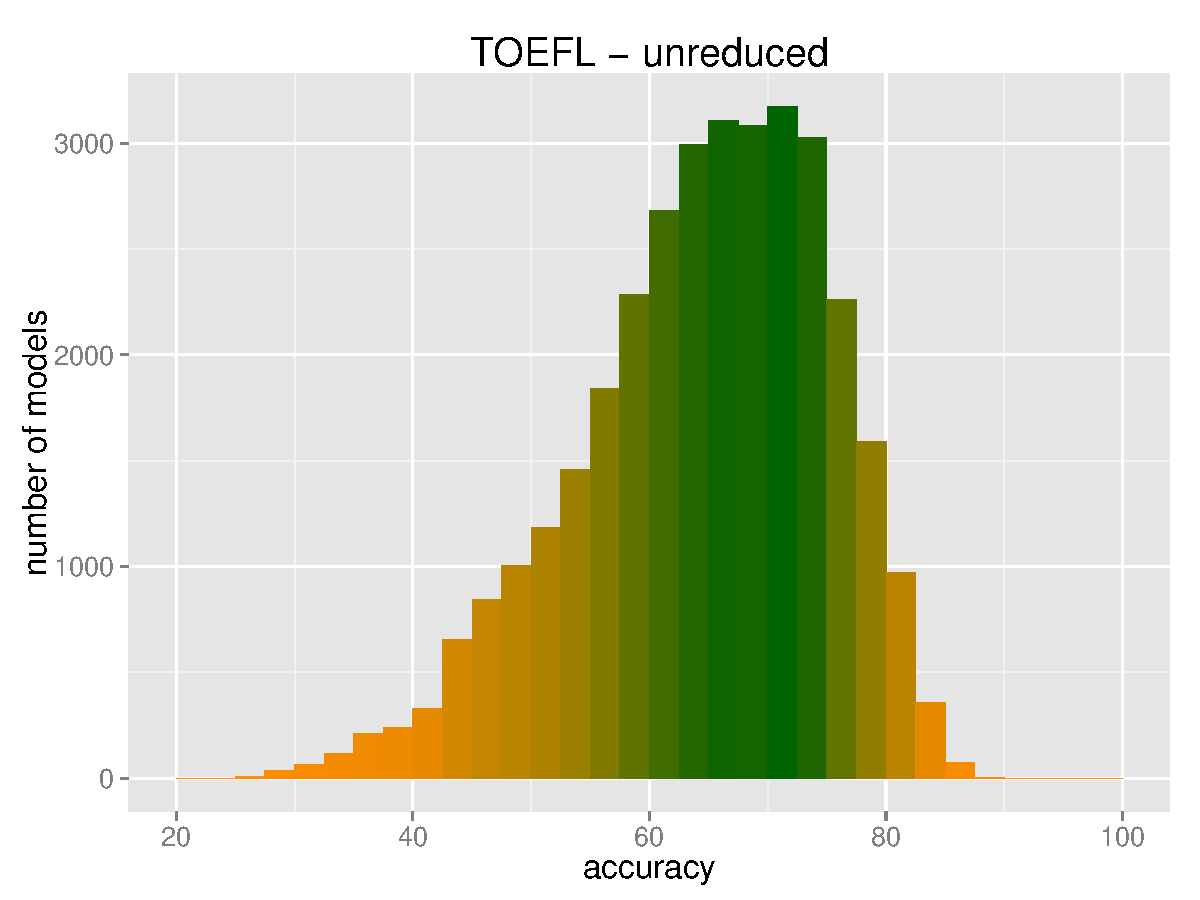
\includegraphics[scale=0.30]{img/lapesa_hist_toefl_unreduced}
      \begin{block}{}\footnotesize \centering
        Min:  25 ; Max: 87.5 ;  Mean: 63.9
      \end{block}
    \end{column}
    \begin{column}{0.5\textwidth}
      \hspace*{-18pt} 
      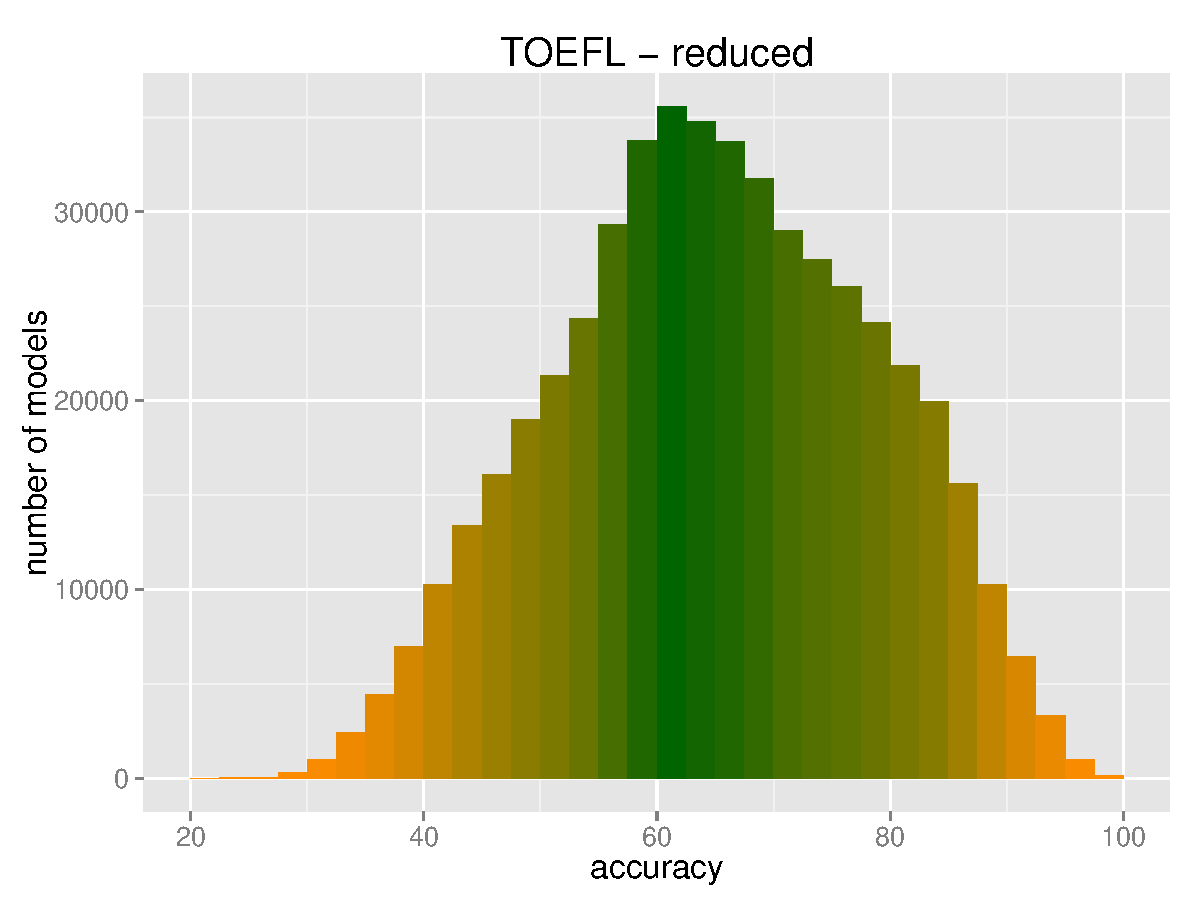
\includegraphics[scale=0.30]{img/lapesa_hist_toefl_reduced}
      \begin{block}{}\footnotesize \centering
        Min:  18.7; Max: \primary{97.4};  Mean: 64.4
      \end{block}
    \end{column}
  \end{columns}
\end{frame}

\begin{frame}
  \frametitle{TOEFL task: parameters and explained variance}
  \framesubtitle{Reduced setting: feature Ablation  (model $R^{2}$: 89\%)}
  \centering
  \hspace*{-10pt}
  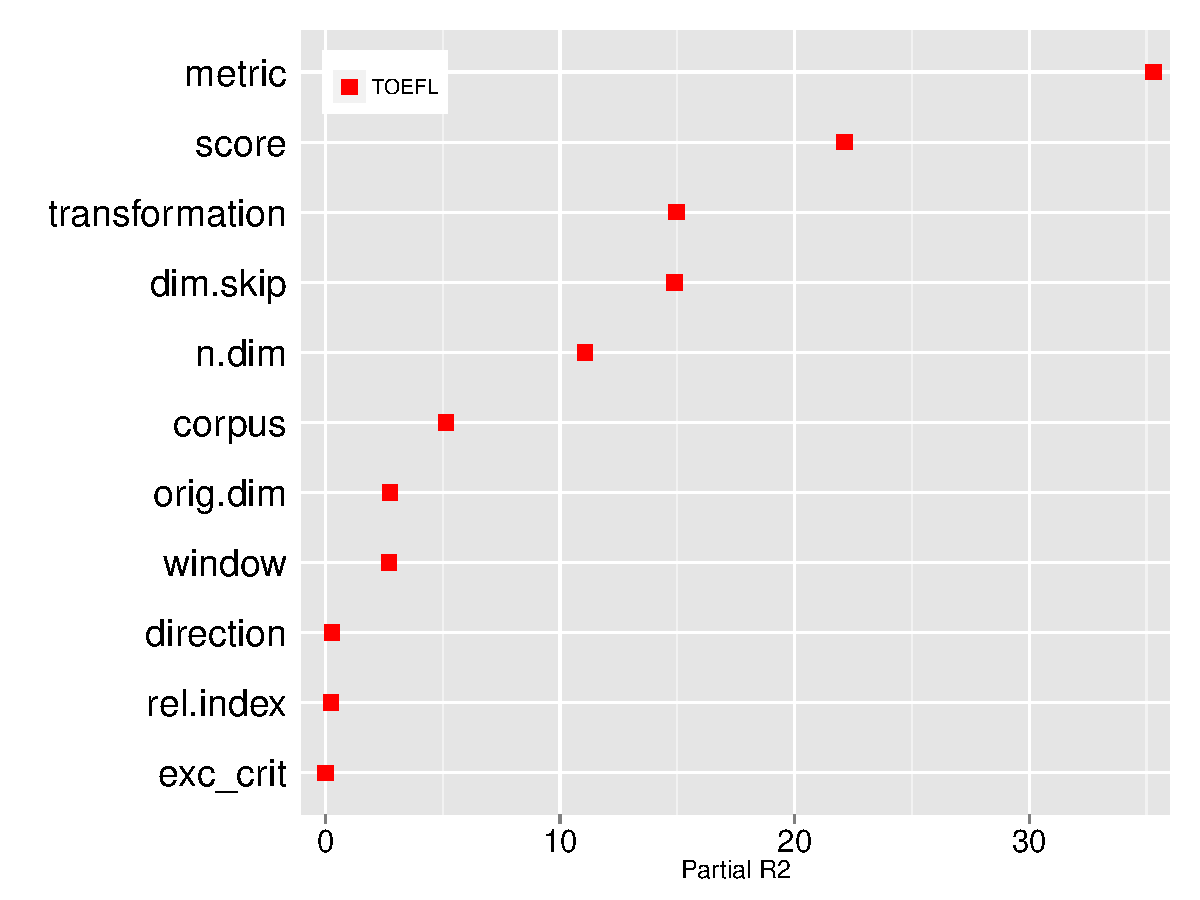
\includegraphics[scale=0.45]{img/lapesa_toefl_main_r2_reduced}

\end{frame}

\begin{frame}
  \frametitle{TOEFL task: interactions}
  \framesubtitle{Reduced setting ($R^{2}$ $>$ 0.5)}

  \begin{center}
    \begin{tabular}{lrrrr}
      Interaction & Df &  R$^2$  \\ \hline
      \primary{score:transformation} & 18  & 7.42 \\   
      \primary{metric:dim.skip} & 2  & 4.44 \\ 
      \primary{score:metric} & 6  & 1.77 \\ 
      metric:orig.dim & 4  & 0.98 \\ 
      window:transformation & 12  & 0.91 \\     
      corpus:score & 12  & 0.84 \\  
      score:orig.dim & 24  & 0.64  \\ 
      metric:n.dim & 4  & 0.63  \\ 
    \end{tabular}

    \gap[1]
    \secondary{TOEFL task: interactions, $R^2$}
  \end{center}  
\end{frame}

\begin{frame}
  \frametitle{TOEFL task: Metric, Score, Transformation}
  \framesubtitle{Partial effect displays \citep{Fox:03}} 

  \centering
  \only<beamer:1-2| handout:0>{\ungap[1]}%
  \only<beamer:1| handout:0>{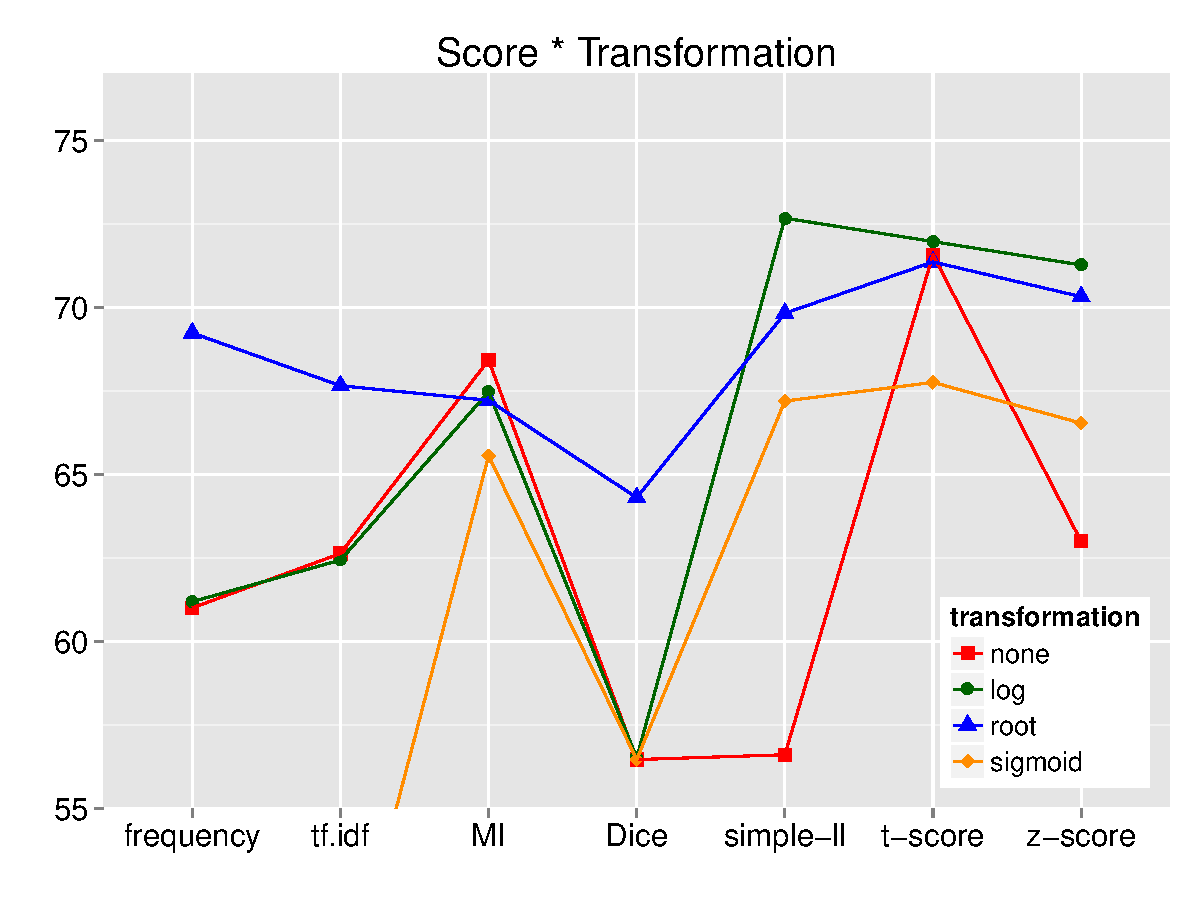
\includegraphics[scale=0.48]{img/lapesa_toefl_main_score_transformation}}%
  \only<beamer:2| handout:0>{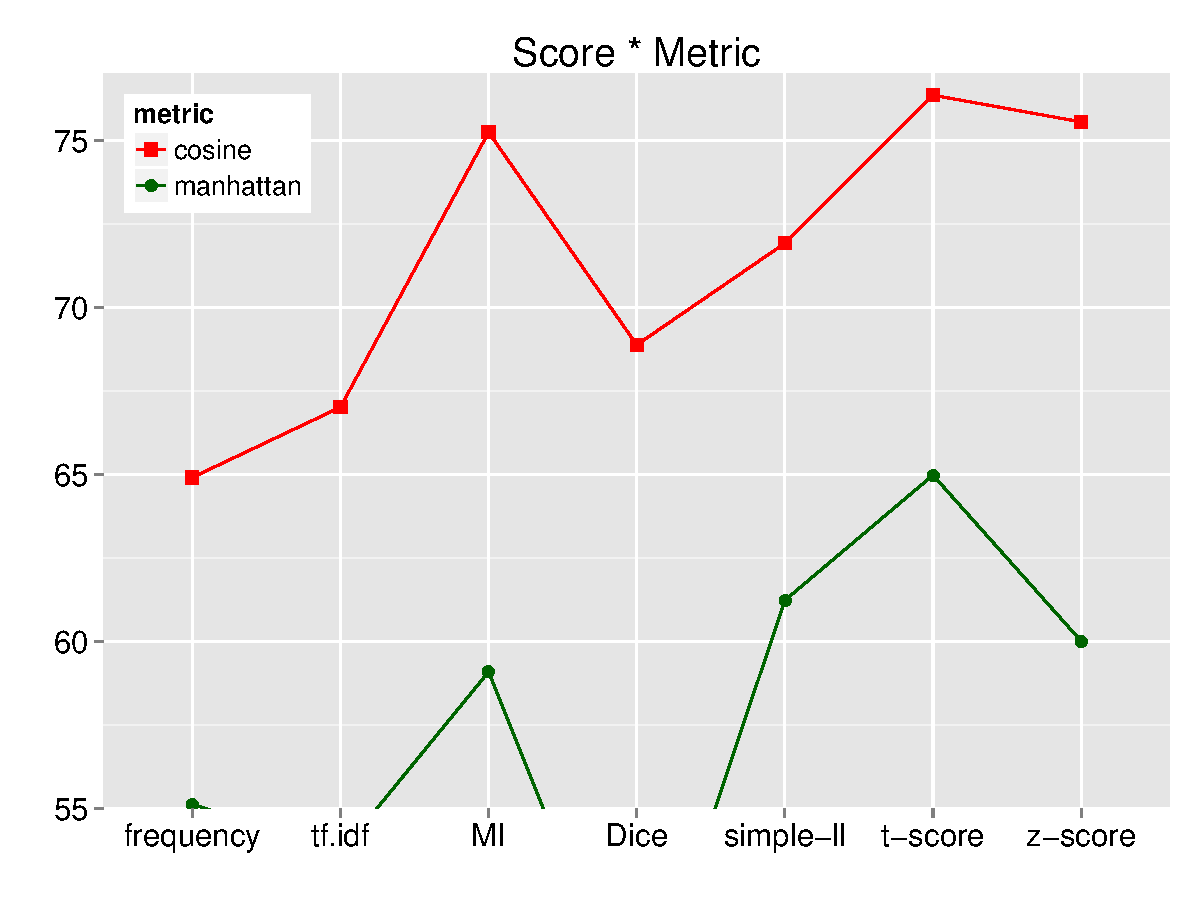
\includegraphics[scale=0.48]{img/lapesa_toefl_main_score_metric}}%
  \only<beamer:0| handout:1>{
    \gap[1]\hspace*{-1cm}%
    \begin{tabular}{c@{}c}
      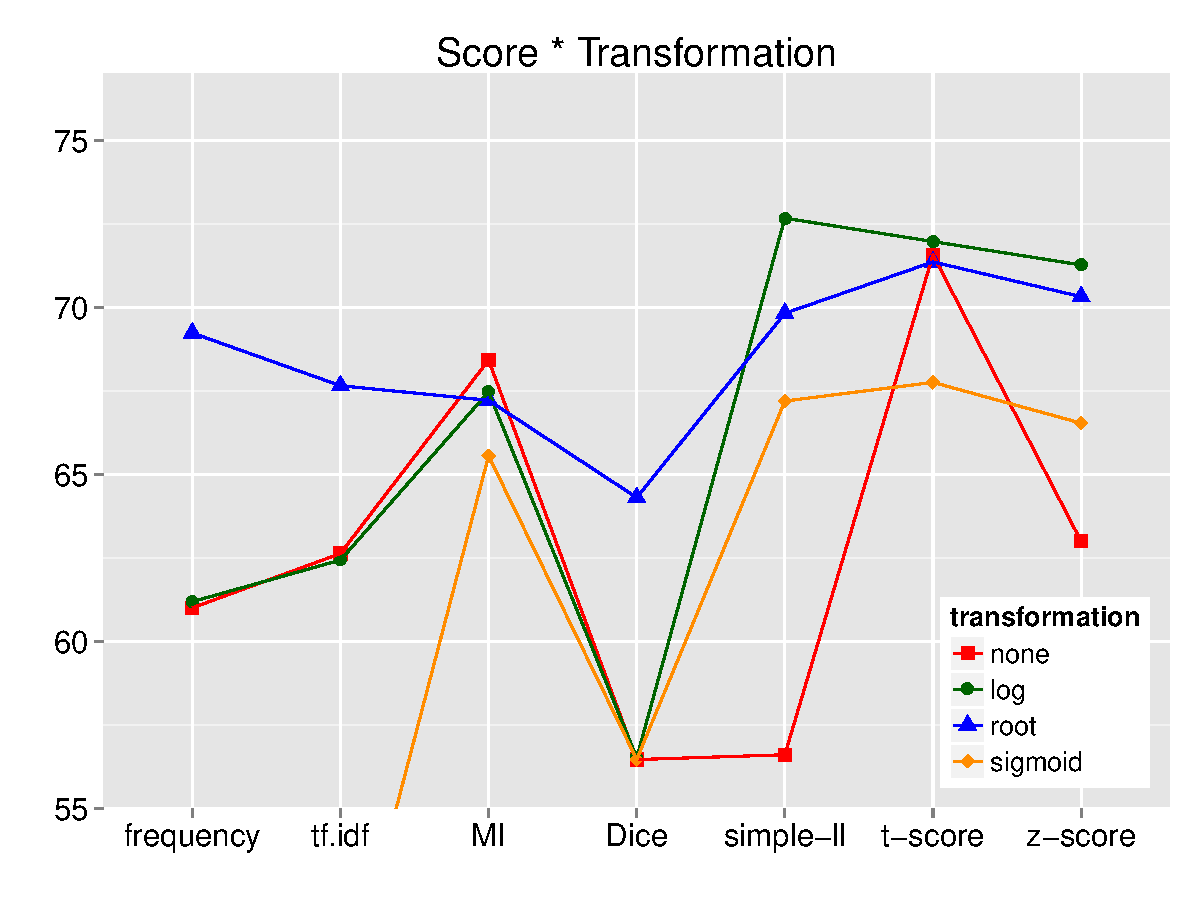
\includegraphics[scale=0.30]{img/lapesa_toefl_main_score_transformation} &
      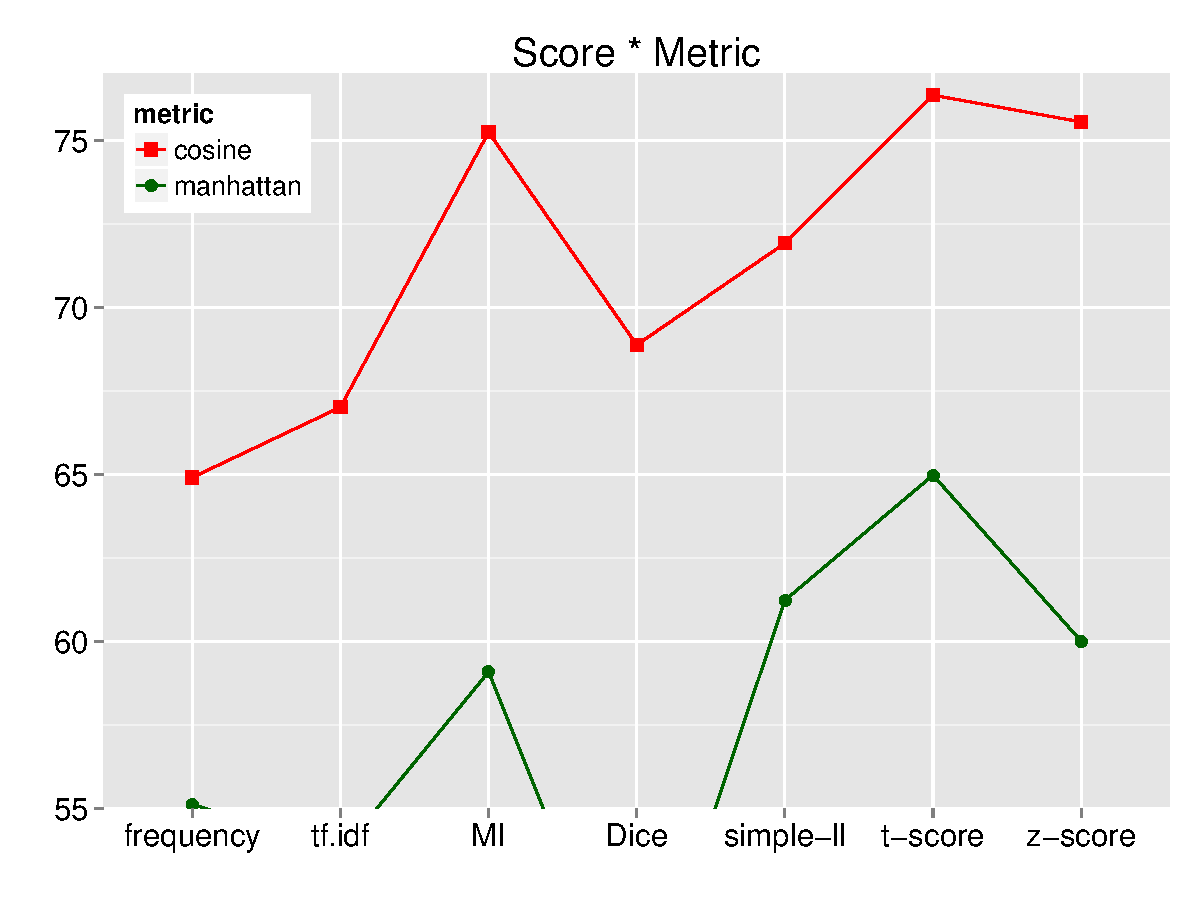
\includegraphics[scale=0.30]{img/lapesa_toefl_main_score_metric}
    \end{tabular}
  }
\end{frame}

\begin{frame}
  \frametitle{TOEFL task: Dimensionality Reduction}
  \framesubtitle{Partial effect displays \citep{Fox:03}} 

  \centering
  \only<beamer:1-2| handout:0>{\ungap[1]}%
  \only<beamer:1| handout:0>{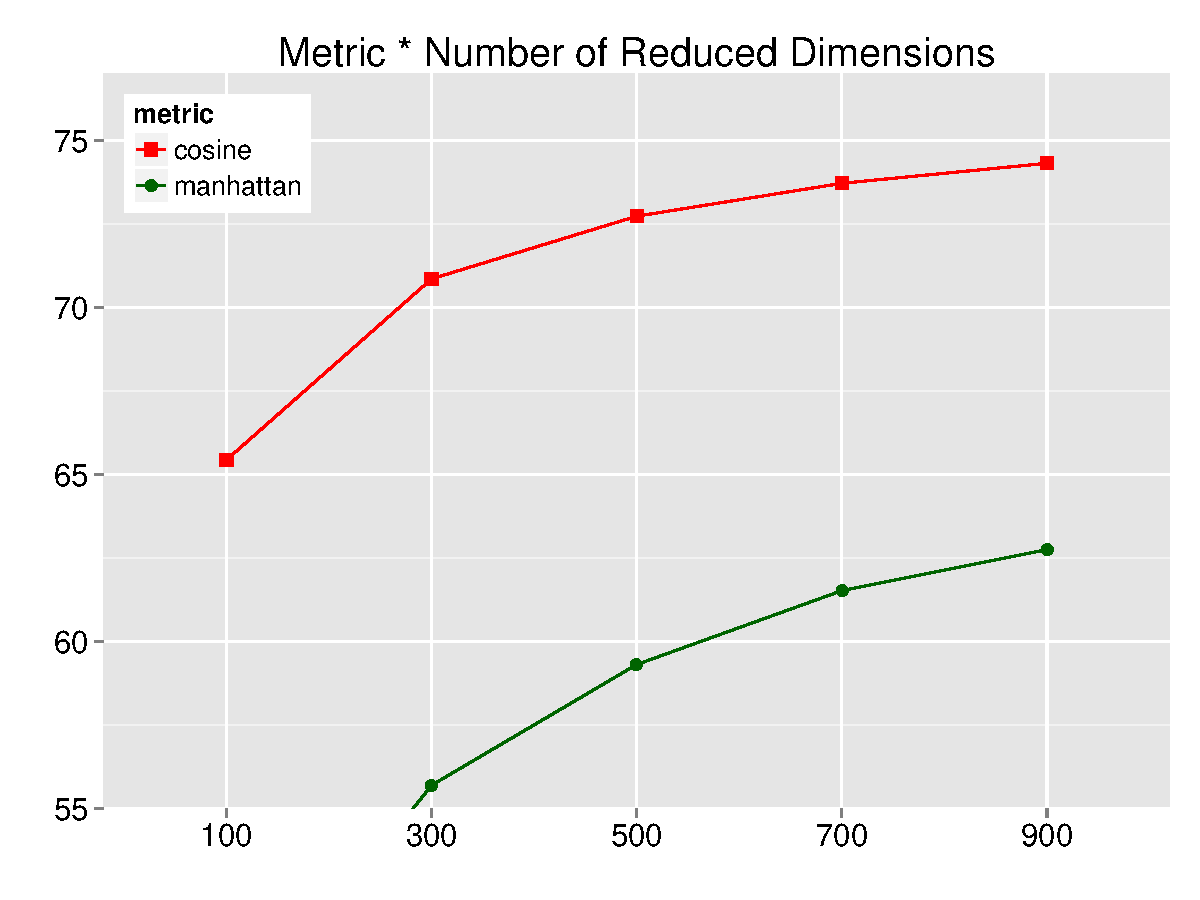
\includegraphics[scale=0.48]{img/lapesa_toefl_main_metric_n-dim}}%
  \only<beamer:2| handout:0>{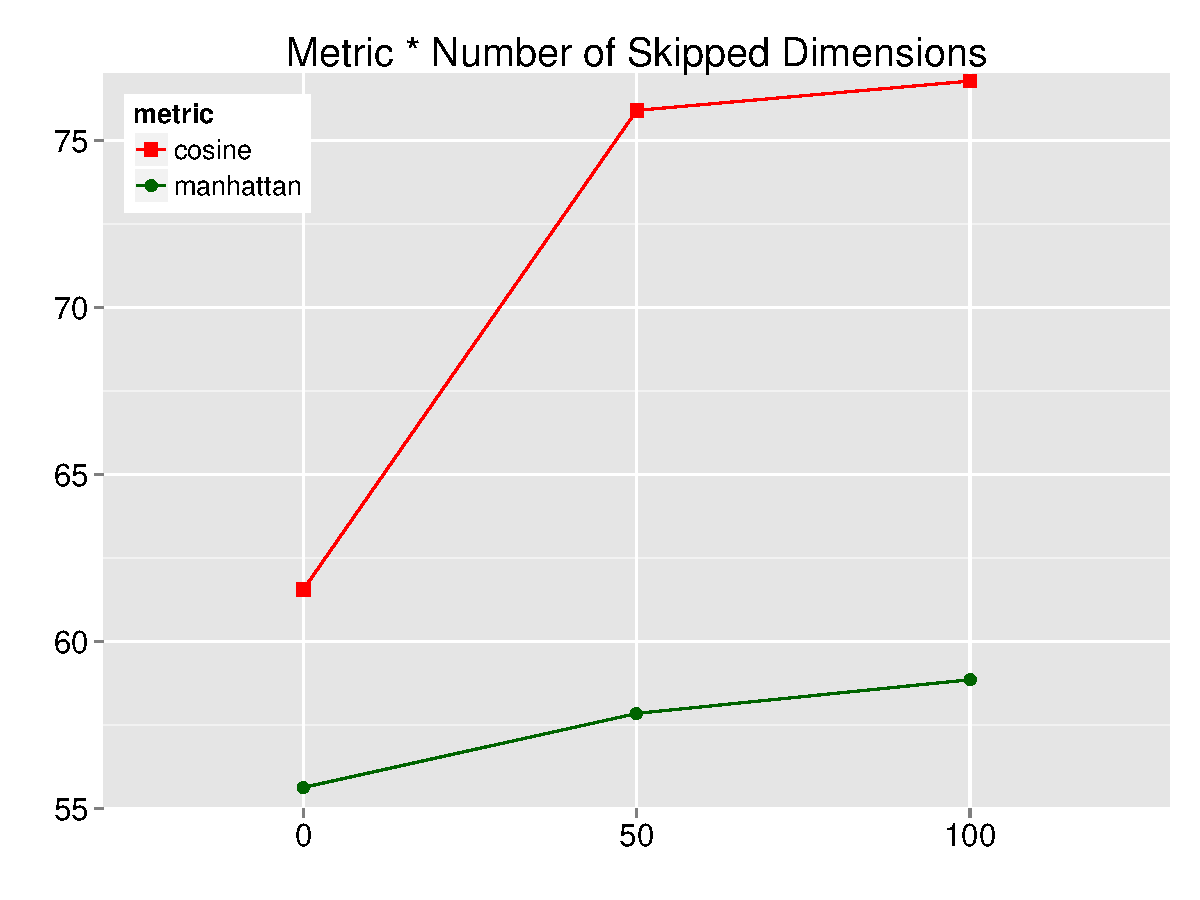
\includegraphics[scale=0.48]{img/lapesa_toefl_main_metric_dim-skip}}%
  \only<beamer:0| handout:1>{
    \gap[1]\hspace*{-1cm}%
    \begin{tabular}{c@{}c}
      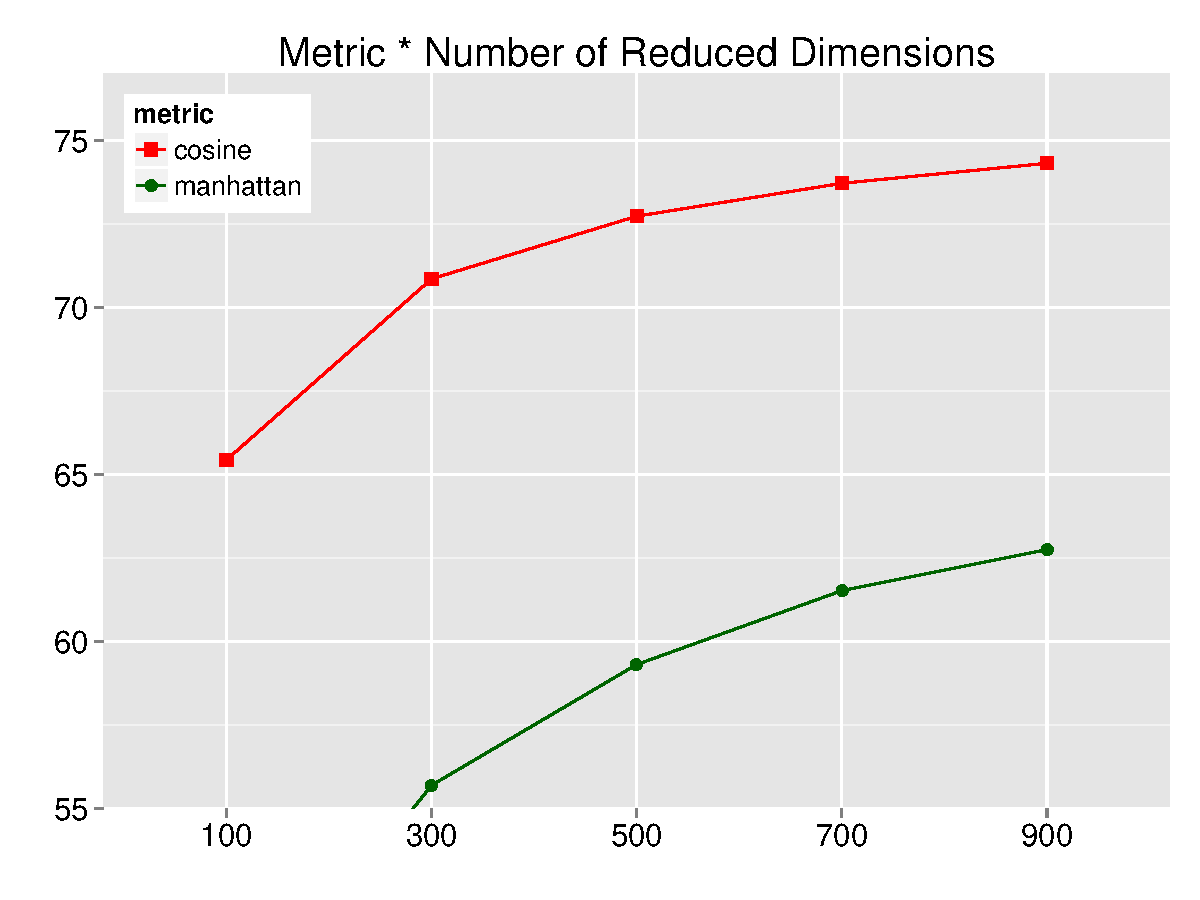
\includegraphics[scale=0.30]{img/lapesa_toefl_main_metric_n-dim} &
      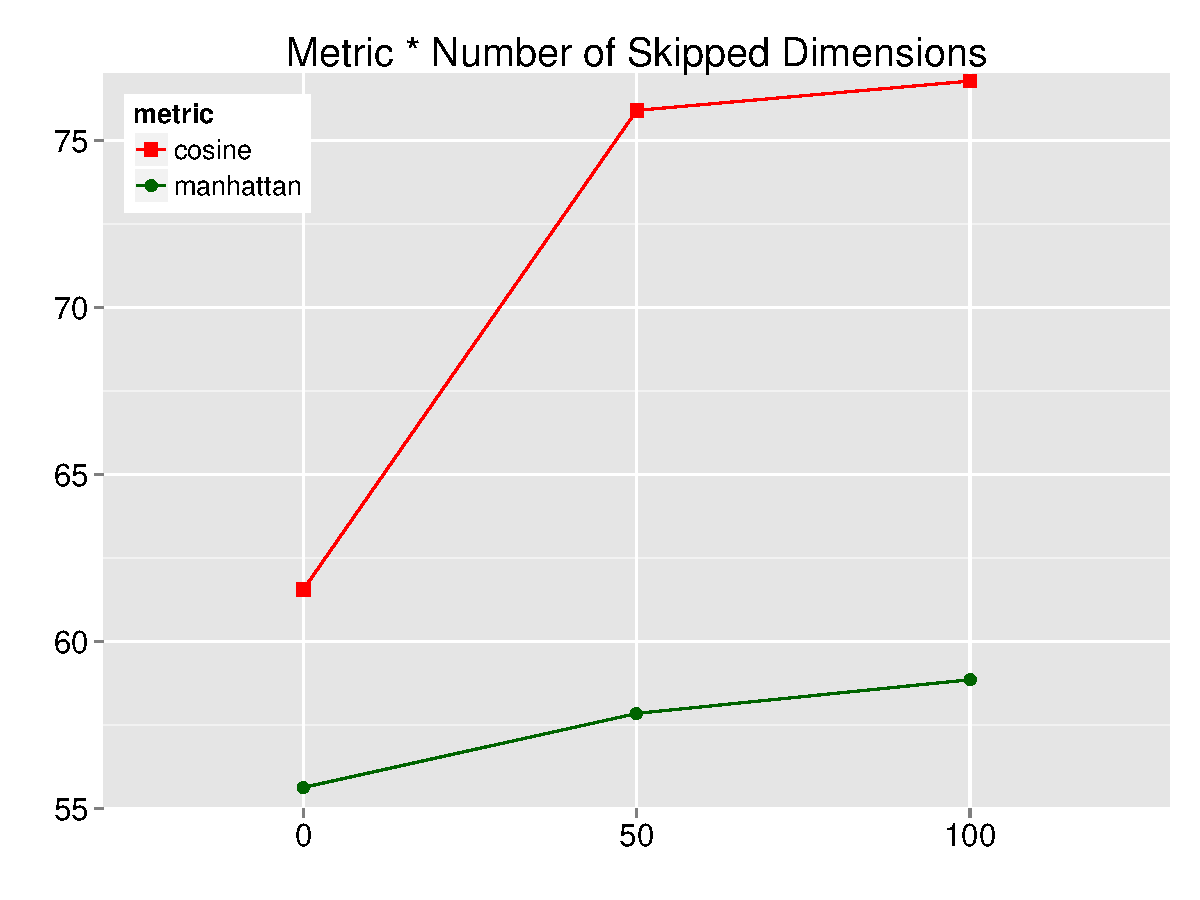
\includegraphics[scale=0.30]{img/lapesa_toefl_main_metric_dim-skip}
    \end{tabular}
  }
\end{frame}

\begin{frame}
  \frametitle{TOEFL task: Corpus and Number of Feature Dimensions}
  \framesubtitle{Partial effect displays \citep{Fox:03}} 

  \centering
  \only<beamer:1-2| handout:0>{\ungap[1]}%
  \only<beamer:1| handout:0>{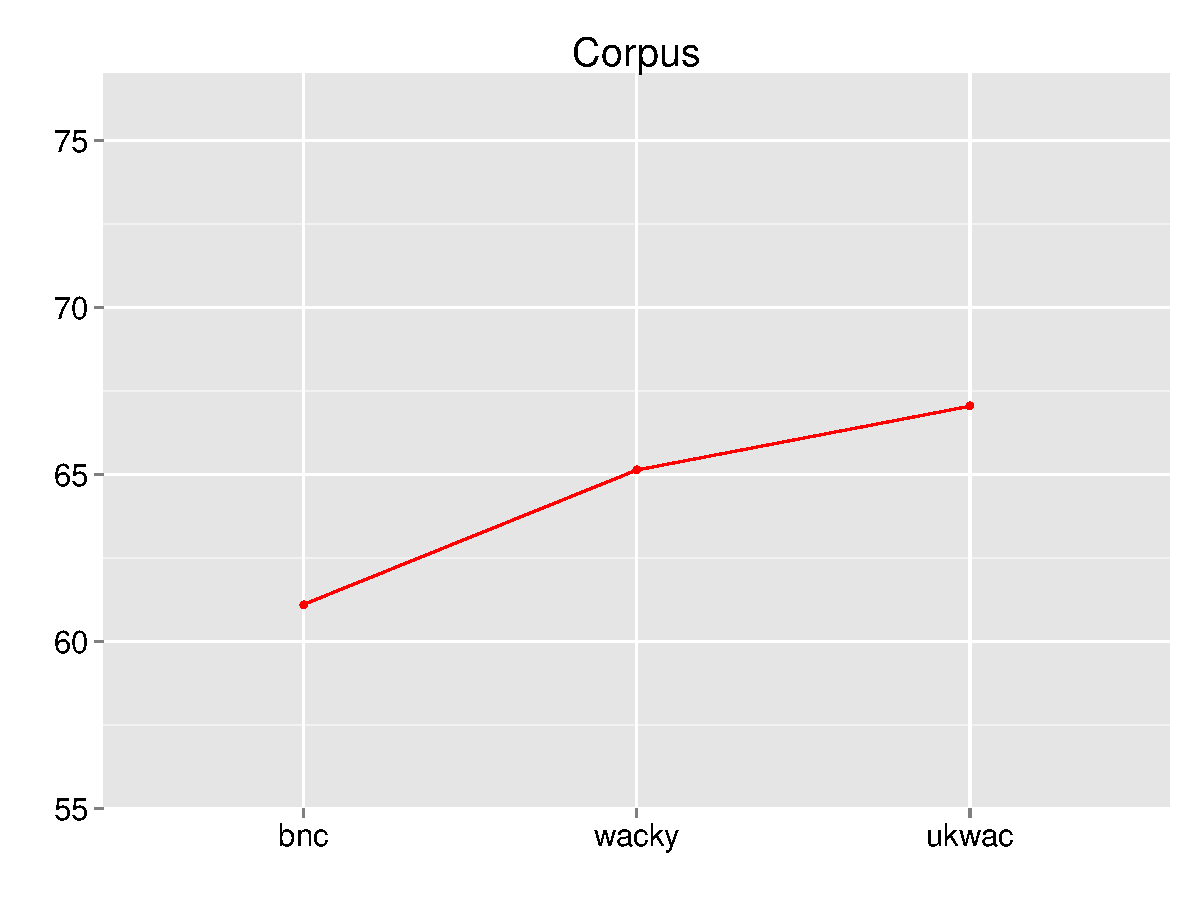
\includegraphics[scale=0.48]{img/lapesa_toefl_main_corpus}}%
  \only<beamer:2| handout:0>{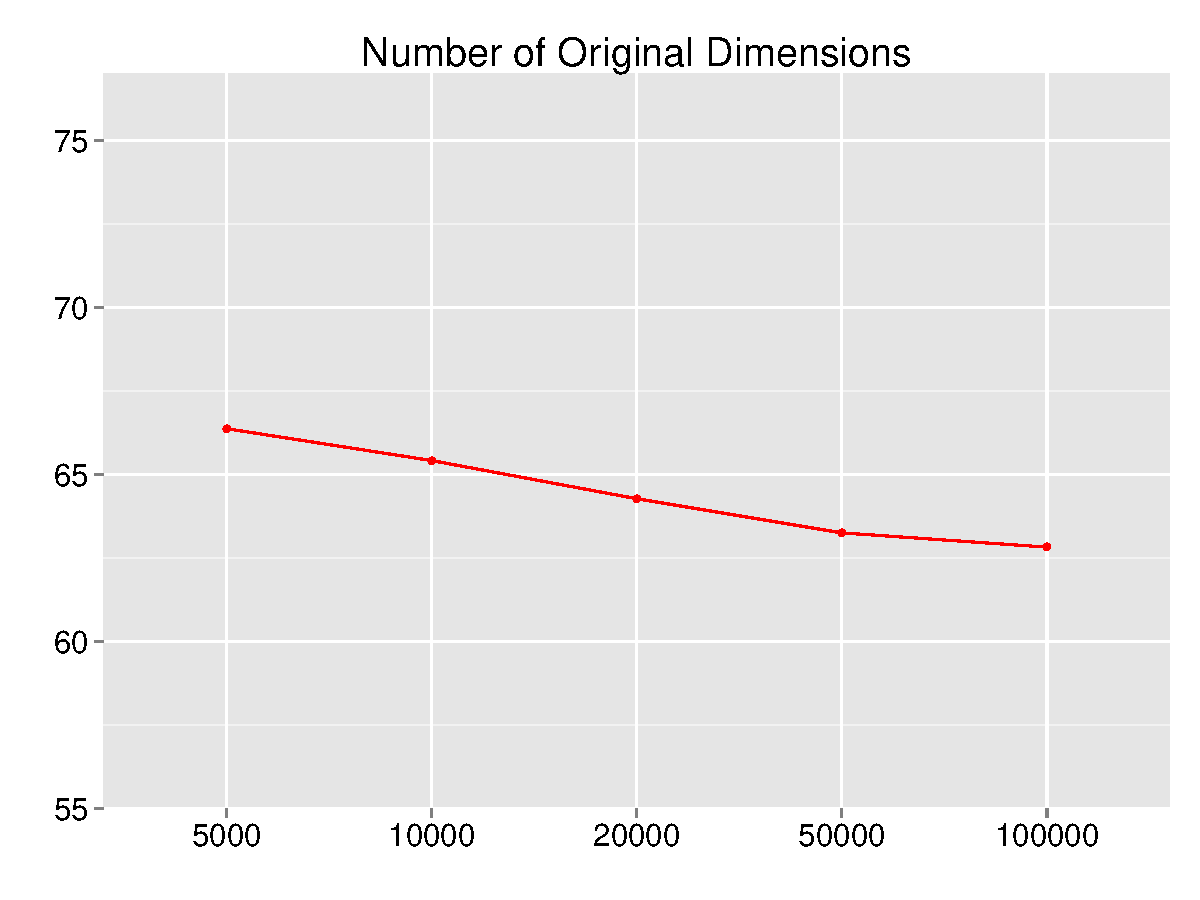
\includegraphics[scale=0.48]{img/lapesa_toefl_main_origdim}}%
  \only<beamer:0| handout:1>{
    \gap[1]\hspace*{-1cm}%
    \begin{tabular}{c@{}c}
      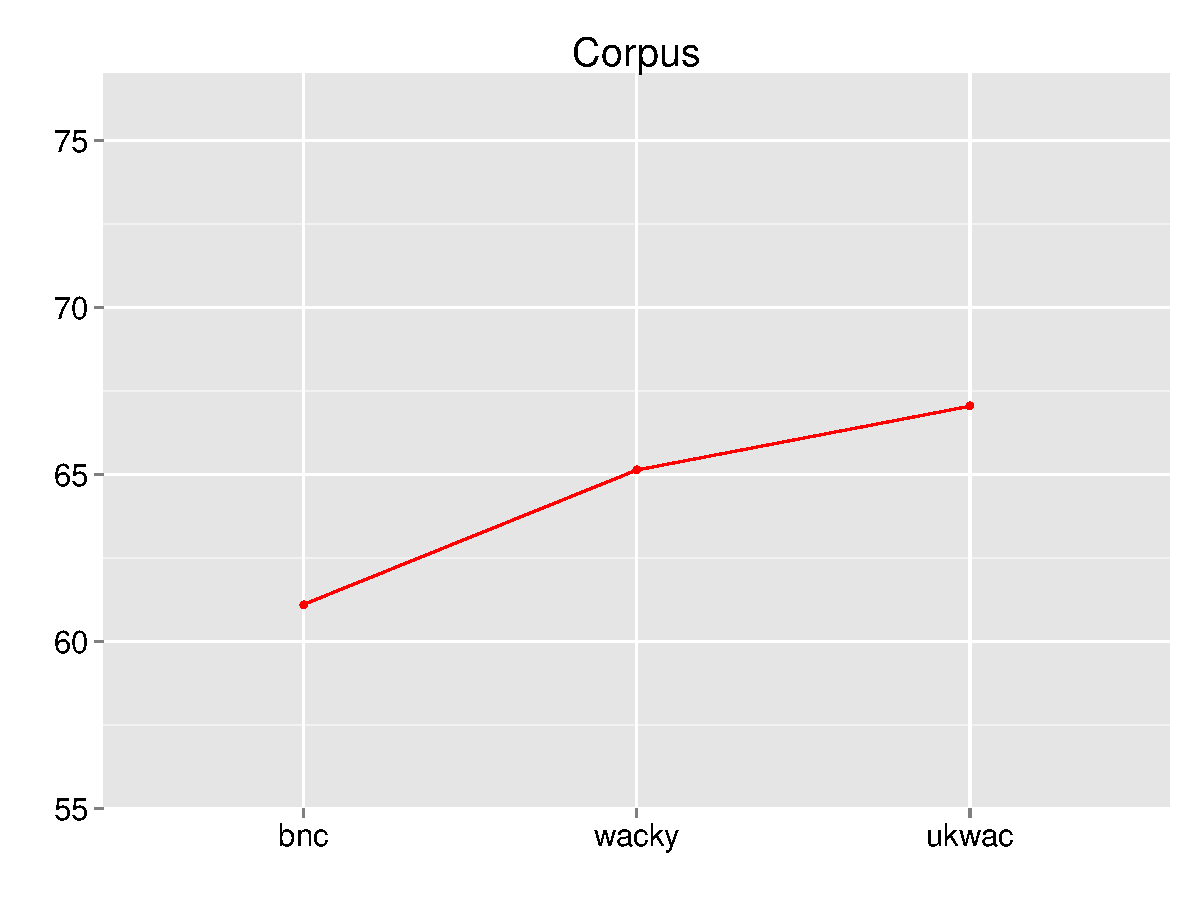
\includegraphics[scale=0.30]{img/lapesa_toefl_main_corpus} &
      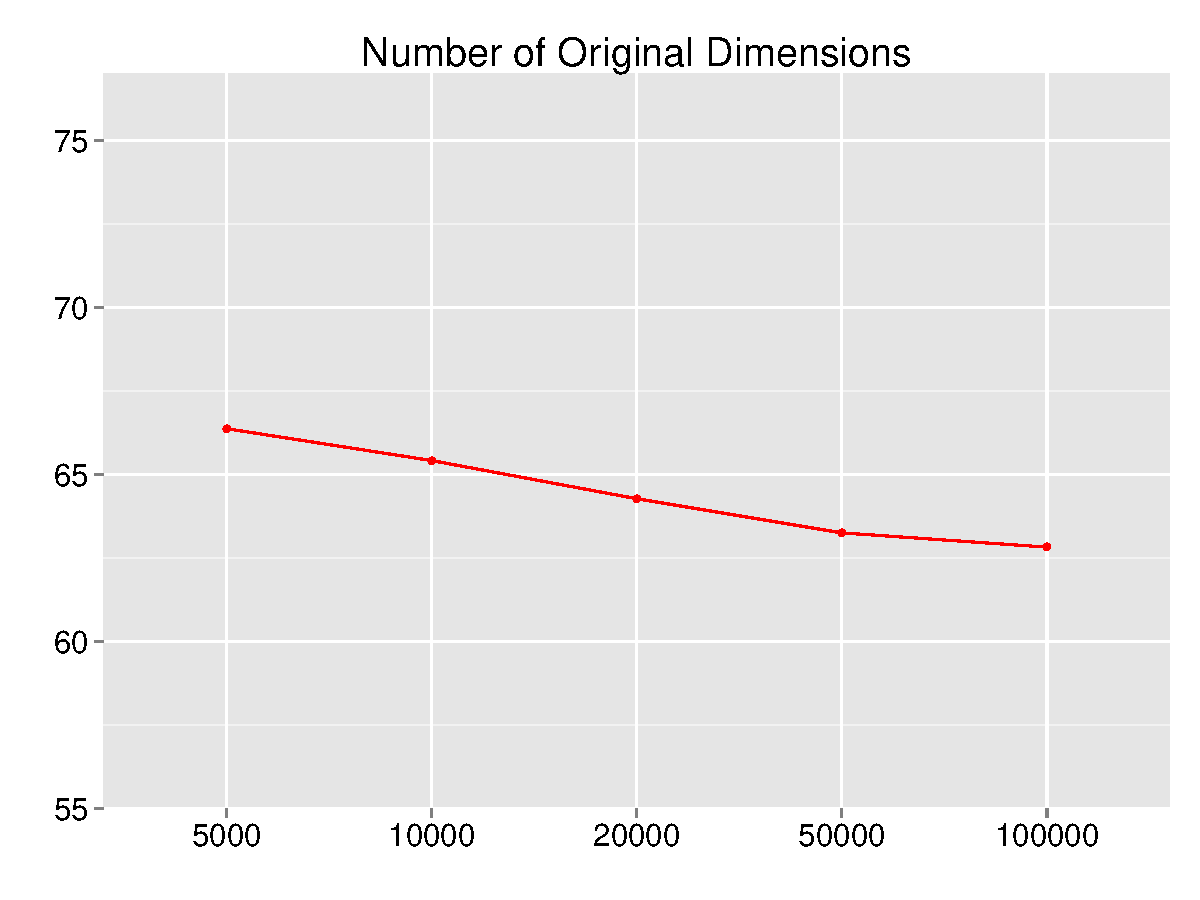
\includegraphics[scale=0.30]{img/lapesa_toefl_main_origdim}
    \end{tabular}
  }
\end{frame}

\begin{frame}
  \frametitle{TOEFL task: Window and Relatedness Index}
  \framesubtitle{Partial effect displays \citep{Fox:03}} 

  \centering
  \only<beamer:1-2| handout:0>{\ungap[1]}%
  \only<beamer:1| handout:0>{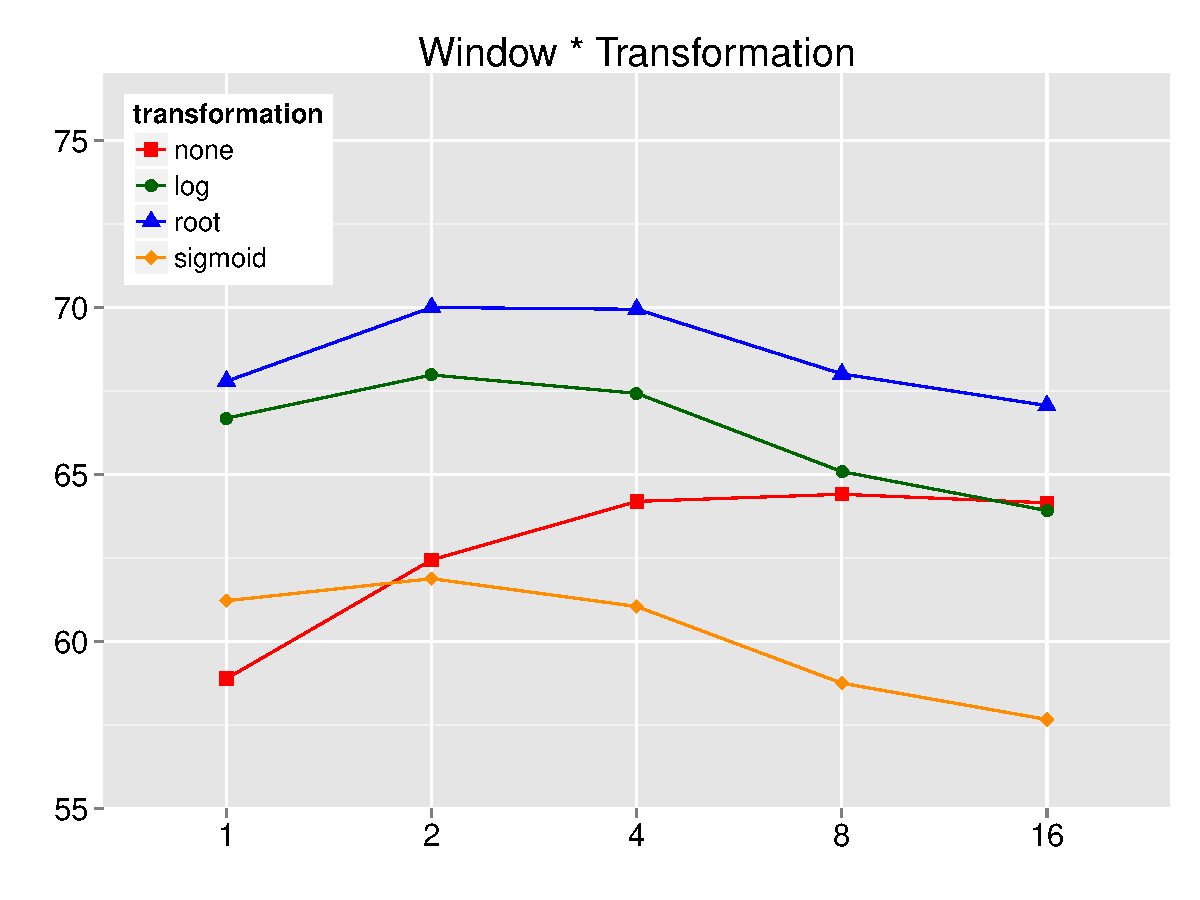
\includegraphics[scale=0.48]{img/lapesa_toefl_main_window_transformation}}%
  \only<beamer:2| handout:0>{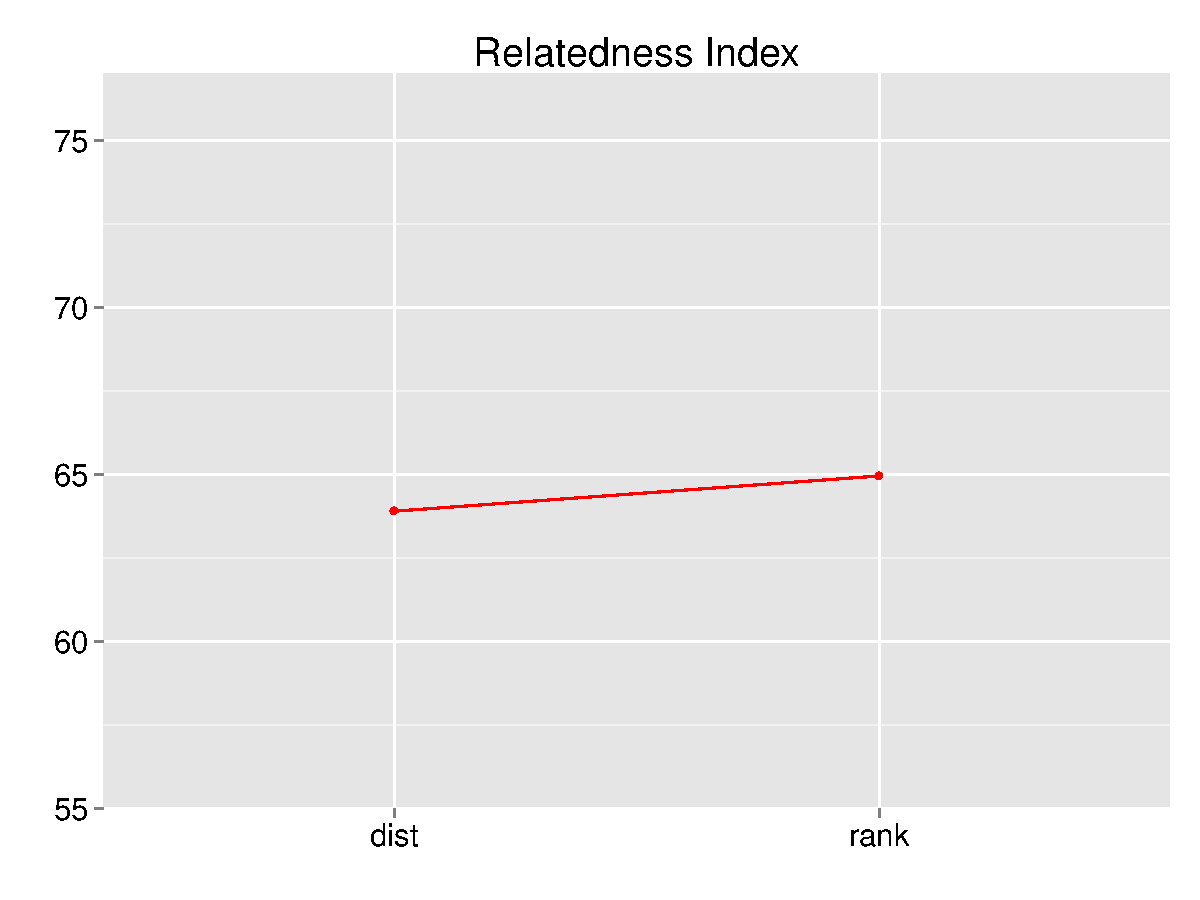
\includegraphics[scale=0.48]{img/lapesa_toefl_main_relindex}}%
  \only<beamer:0| handout:1>{
    \gap[1]\hspace*{-1cm}%
    \begin{tabular}{c@{}c}
      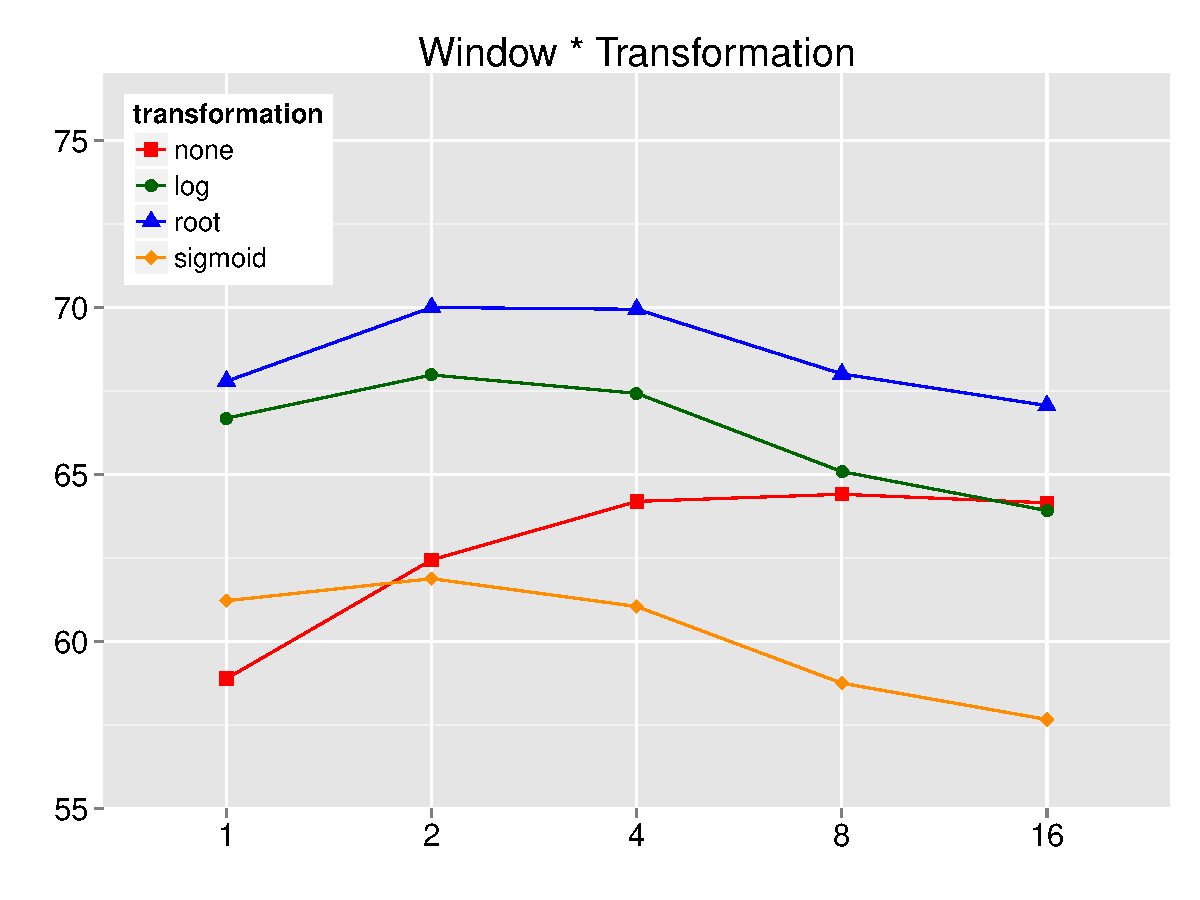
\includegraphics[scale=0.30]{img/lapesa_toefl_main_window_transformation} &
      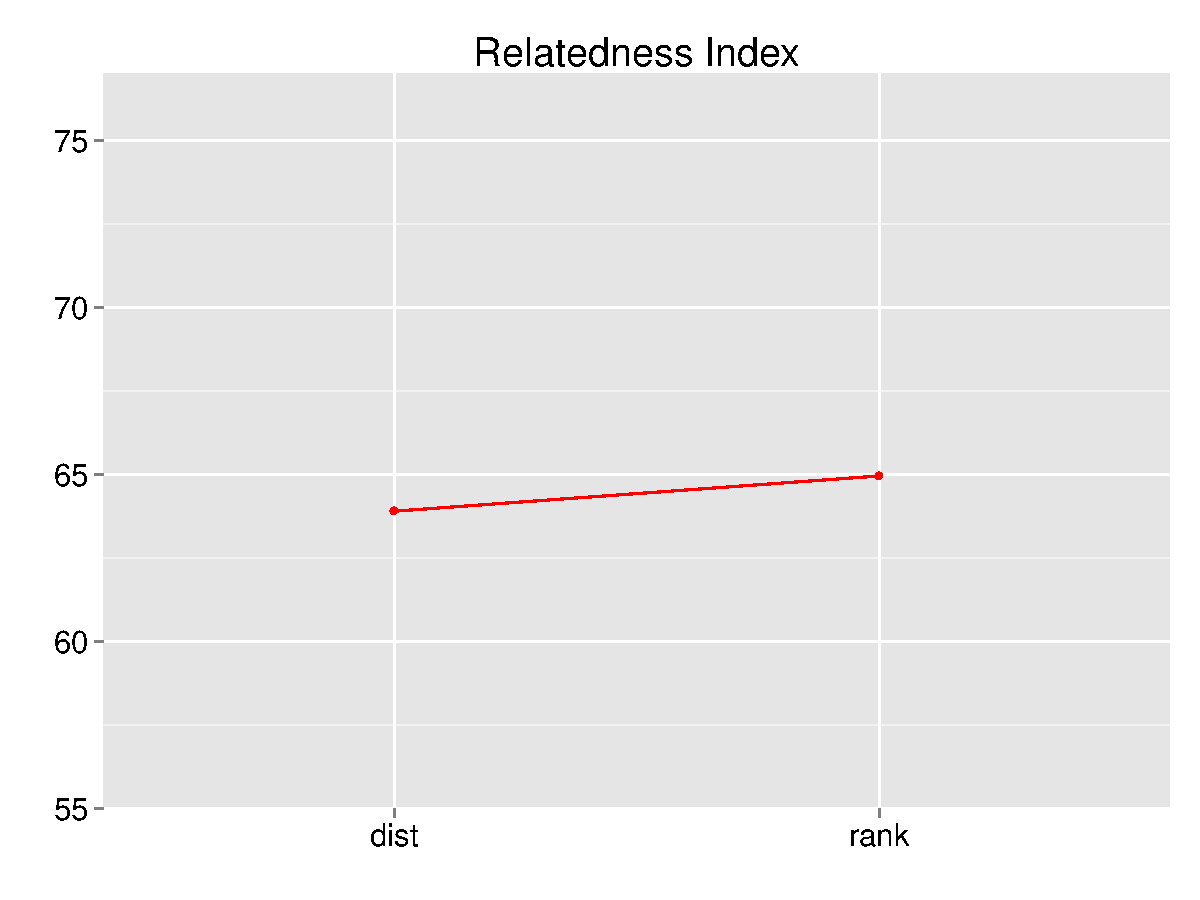
\includegraphics[scale=0.30]{img/lapesa_toefl_main_relindex}
    \end{tabular}
  }
\end{frame}

\begin{frame}
  \frametitle{TOEFL task: summary}
  \begin{exampleblock}{TOEFL: best setting}
    \begin{itemize}\footnotesize
    \item Corpus: ukWac
    \item Window: undirected, 2 words 
    \item Feature selection: top 5000/10000 dimensions, based on frequency
    \item Score * Transformation: simple-ll * log
    \item Dimensionality Reduction: 900 latent dimensions, skipping the first 100
    \item Distance Metric: cosine
    \item Index of Distributional Relatedness: neighbor rank
    \end{itemize}
  \end{exampleblock}   
  
\end{frame}


\begin{frame}
  \frametitle{DSMs and similarity ratings}
  \framesubtitle{Introducing the task}

  \ungap[1]
  \begin{columns}
    \begin{column}{0.5\textwidth}
      \begin{exampleblock}{RG65}
        \textbf{65 pairs, rated from 0 to 4}
        \textit{gem -- jewel}: 3.94 \\
        \textit{grin -- smile}:  3.46 \\
        \textit{fruit -- furnace}: 0.05 \\
      \end{exampleblock}
    \end{column}
    % 
    \begin{column}{0.5\textwidth}
      
      
      \begin{exampleblock}  {WordSim353}
        \textbf{353 pairs, rated from 1 to 10}
        \textit{announcement -- news}: 7.56 \\
        \textit{weapon -- secret}:  6.06 \\
        \textit{travel -- activity}: 5.00 \\
      \end{exampleblock}
    \end{column}
    % 
  \end{columns}
  % 
  % 
  \begin{itemize}
  \item A \textbf{prediction} task
  \item If distributional representation are close to  speakers' conceptual representations, we expect to find some \textbf{correlation} between distance in the semantic space and speaker's judgments concerning semantic similarity
  \item Performance: \textbf{Pearson correlation $r$}
  \end{itemize}

\end{frame}

\begin{frame}
  \frametitle{Similarity ratings: performance on RG65}
  \centering
  
  \begin{columns}
    \begin{column}{0.5\textwidth}
      \centering
      \hspace*{-18pt}   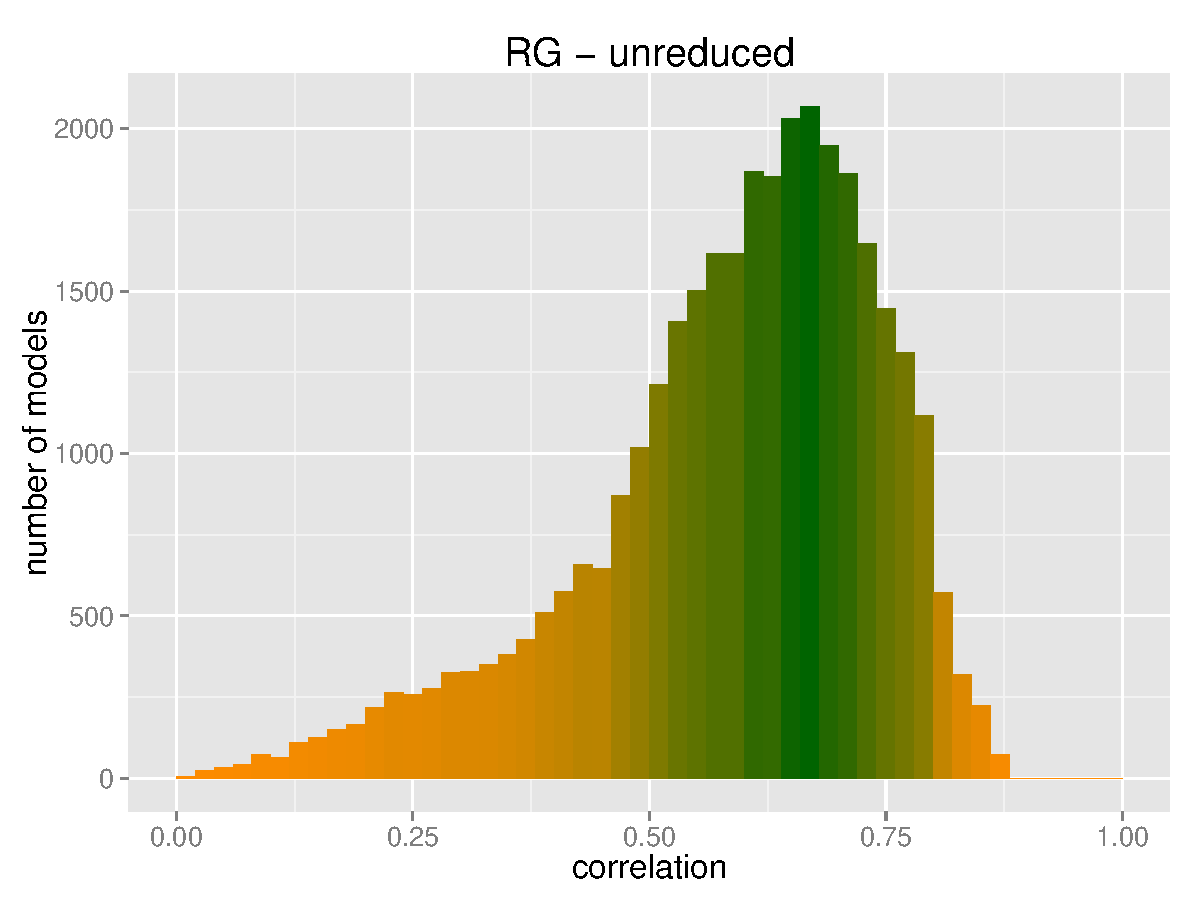
\includegraphics[scale=0.30]{img/lapesa_hist_rg_unreduced}
      \begin{block}{}\footnotesize \centering
        Min:  0.01; Max:  0.88;  Mean 0.59 \\
        \secondary{unreduced}
      \end{block}
    \end{column}
    \begin{column}{0.5\textwidth}
      \hspace*{-18pt} 
      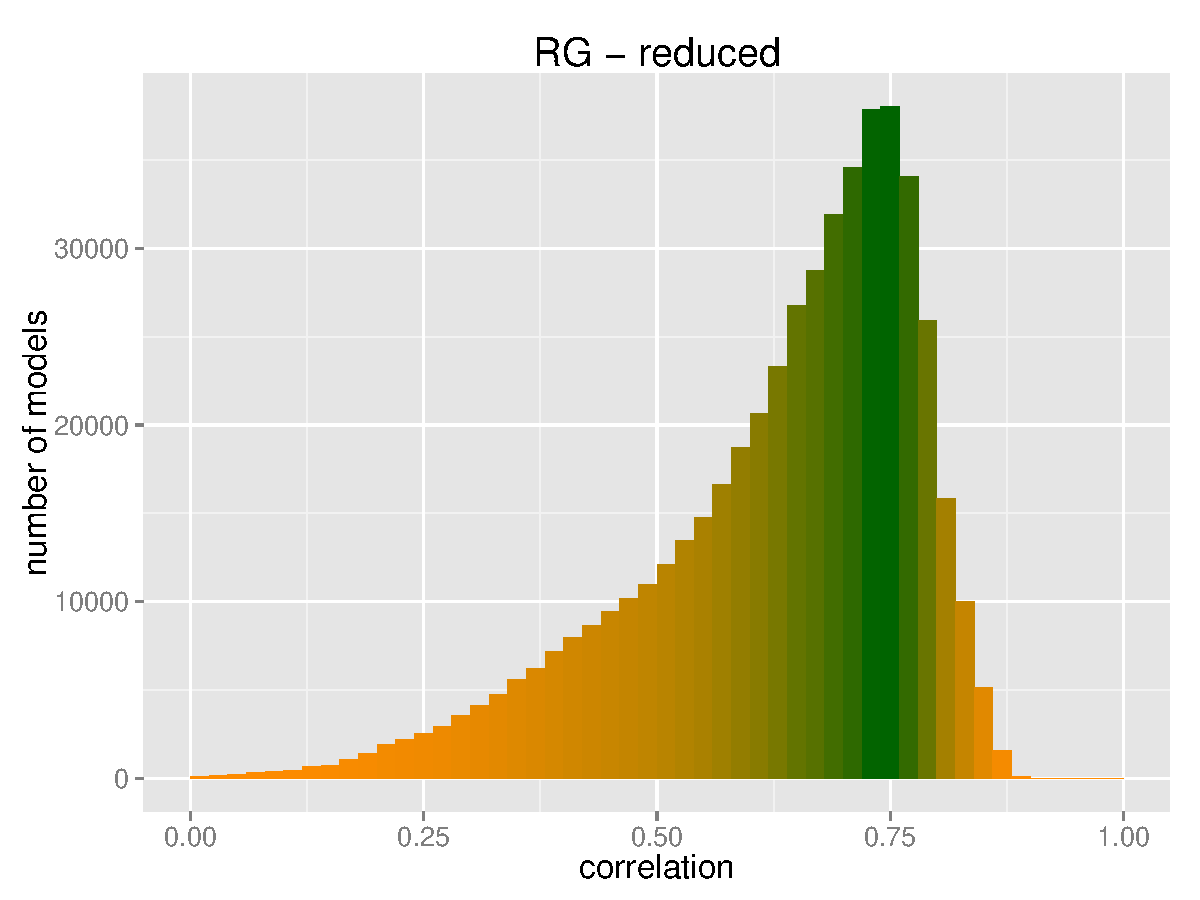
\includegraphics[scale=0.30]{img/lapesa_hist_rg_reduced}
      \begin{block}{}\footnotesize \centering
        Min:  0.00; Max: \primary{0.89};  Mean: 0.63\\
        \secondary{reduced}
      \end{block}
    \end{column}
  \end{columns}
 
\end{frame}

\begin{frame}
  \frametitle{Similarity ratings: performance on WordSim353}
  \centering
  
  \begin{columns}

    \begin{column}{0.5\textwidth}
      \centering
      \hspace*{-18pt} 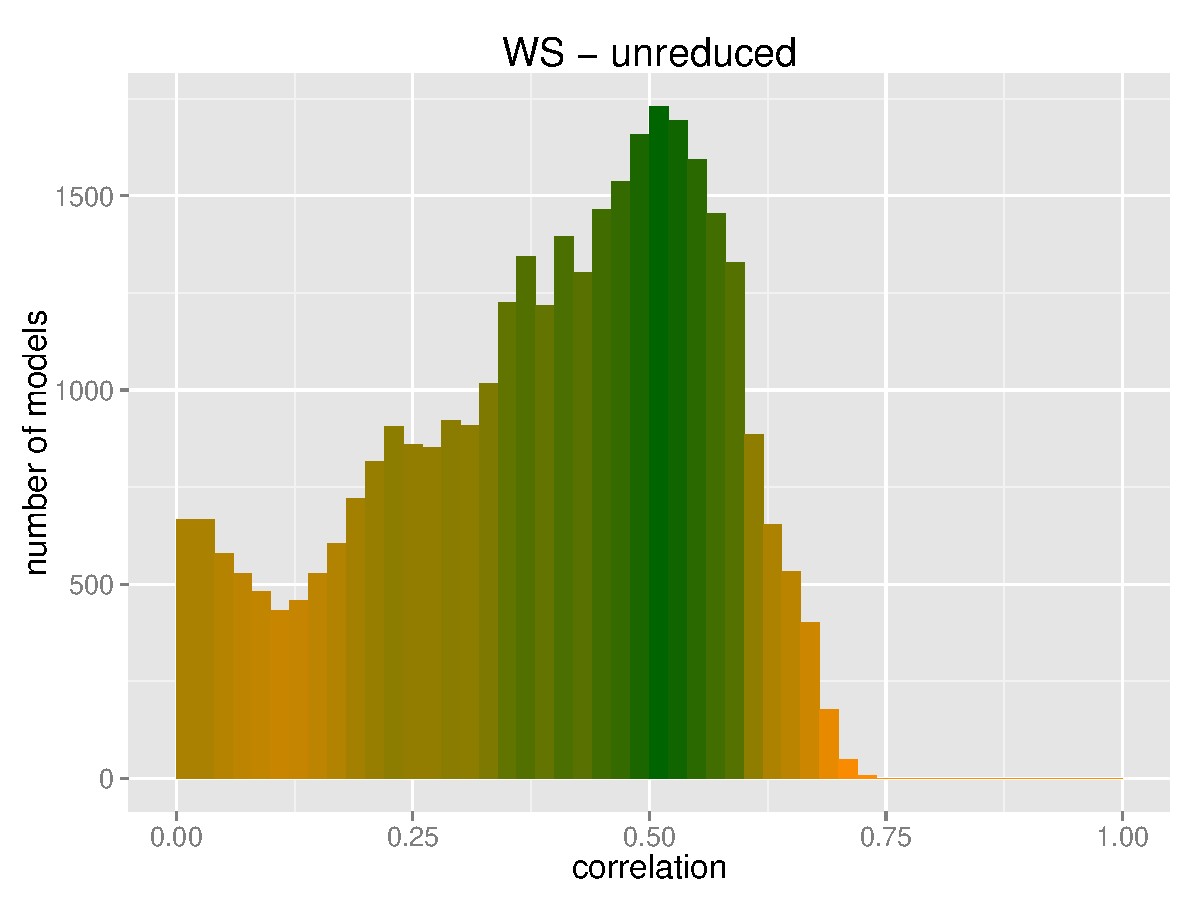
\includegraphics[scale=0.30]{img/lapesa_hist_ws_unreduced}
      \begin{block}{}\footnotesize \centering
        Min:  0.00; Max: \primary{0.73};  Mean: 0.39\\
        \secondary{unreduced}
      \end{block}
    \end{column}
    \begin{column}{0.5\textwidth}
      \hspace*{-18pt} 
      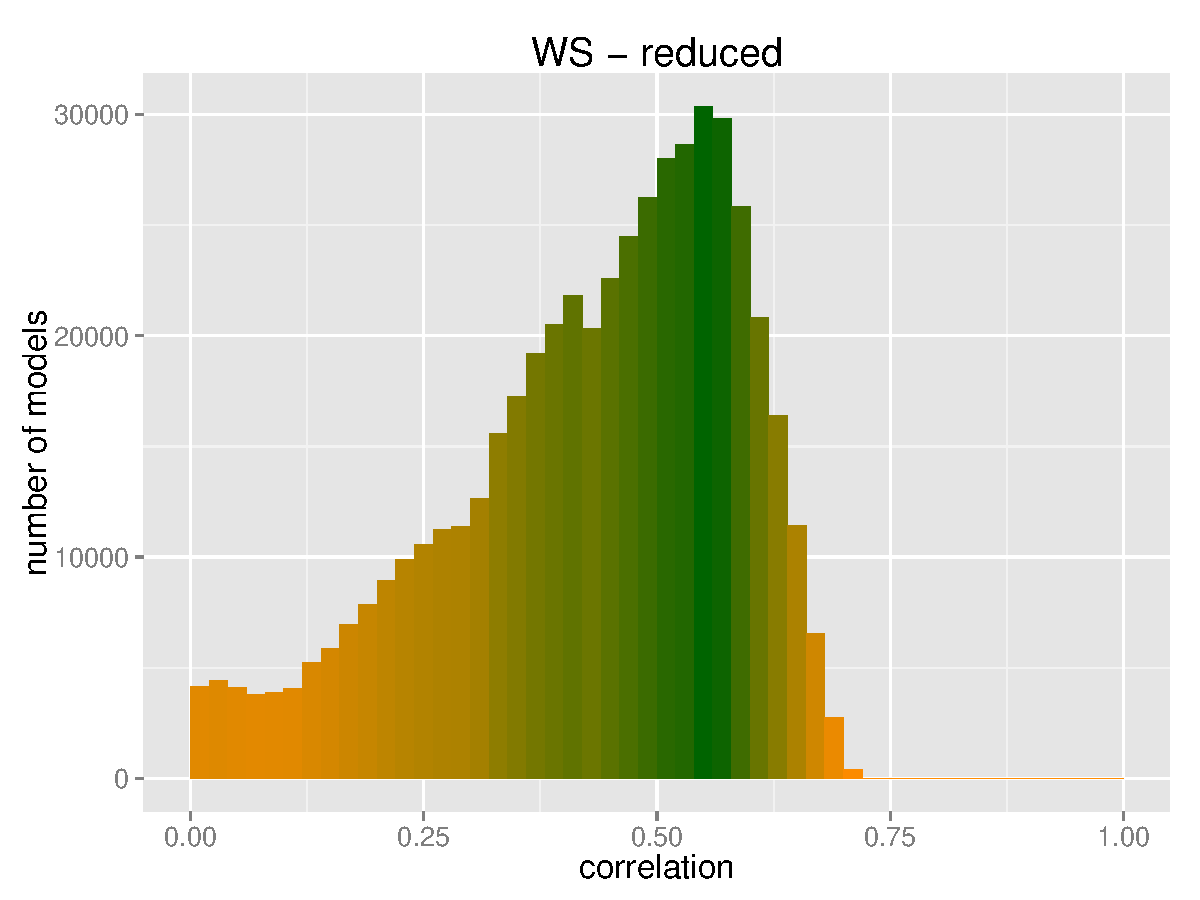
\includegraphics[scale=0.30]{img/lapesa_hist_ws_reduced}
      \begin{block}{}\footnotesize \centering
        Min:  0.00; Max: \primary{0.73};  Mean: 0.43\\
        \secondary{reduced}
      \end{block}
    \end{column}
  \end{columns}  
\end{frame}


\begin{frame}
  \frametitle{Similarity ratings: parameters and explained variance}
  \framesubtitle{Reduced setting: feature ablation  (full model $R^{2}$: RG65 86\%; WS353 90\%)}
  \centering
  \hspace*{-10pt}
  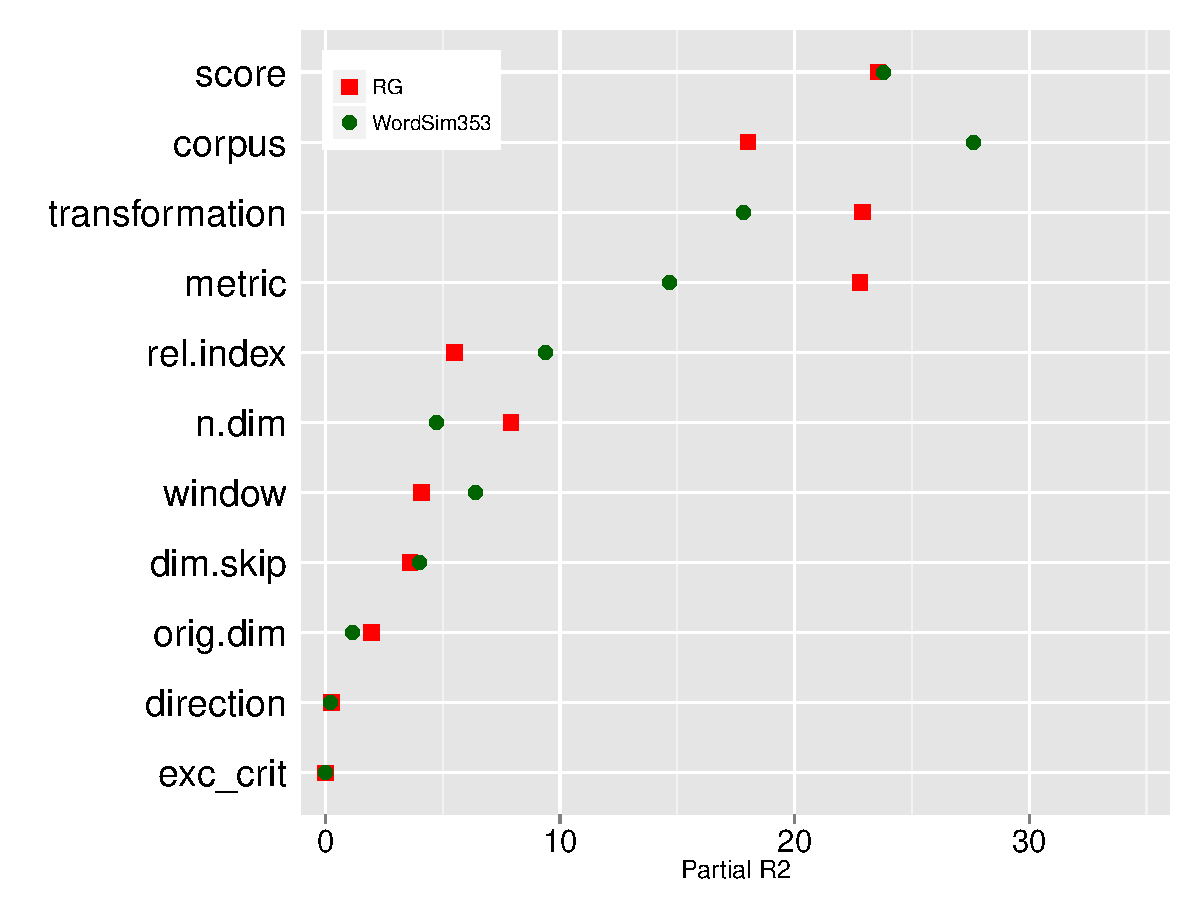
\includegraphics[scale=0.45]{img/lapesa_ratings_main_r2_reduced}

\end{frame}

\begin{frame}
  \frametitle{Similarity ratings: interactions}
  \framesubtitle{Reduced setting ($R^2 > 0.5$)}

  \begin{center}
    \begin{tabular}{lrrrr}
      Interaction & Df & RG65  & WordSim353 \\ \hline

      \primary{score:transf} & 18  & 10.28 & 8.66  \\ 
      \primary{metric:n.dim} & 4  & 2.18 & 1.42 \\   
      \primary{window:transf} & 12  & 1.43 & 1.01 \\   
      corpus:metric & 2  & 1.83 & 0.51 \\  
      score:metric & 6  & 1.91 & 0.59  \\  
      metric:orig.dim & 4  & 1.08 & 0.62 \\ 
      corpus:score & 12 & 0.77 &  0.82 \\ 
      window:score & 24  & 0.77 & 0.69  \\
      score:dim.skip & 12  & 0.58 & 0.85 \\ 
    \end{tabular}

    \gap[1]
    \secondary{Similarity ratings: interactions, $R^2$} 
  \end{center}

\end{frame}


\begin{frame}
  \frametitle{Similarity ratings: Score, Transformation}
  \framesubtitle{Partial effect displays \citep{Fox:03}} 

  \centering
  \gap[1]\hspace*{-1cm}%
  \begin{tabular}{c@{}c}
    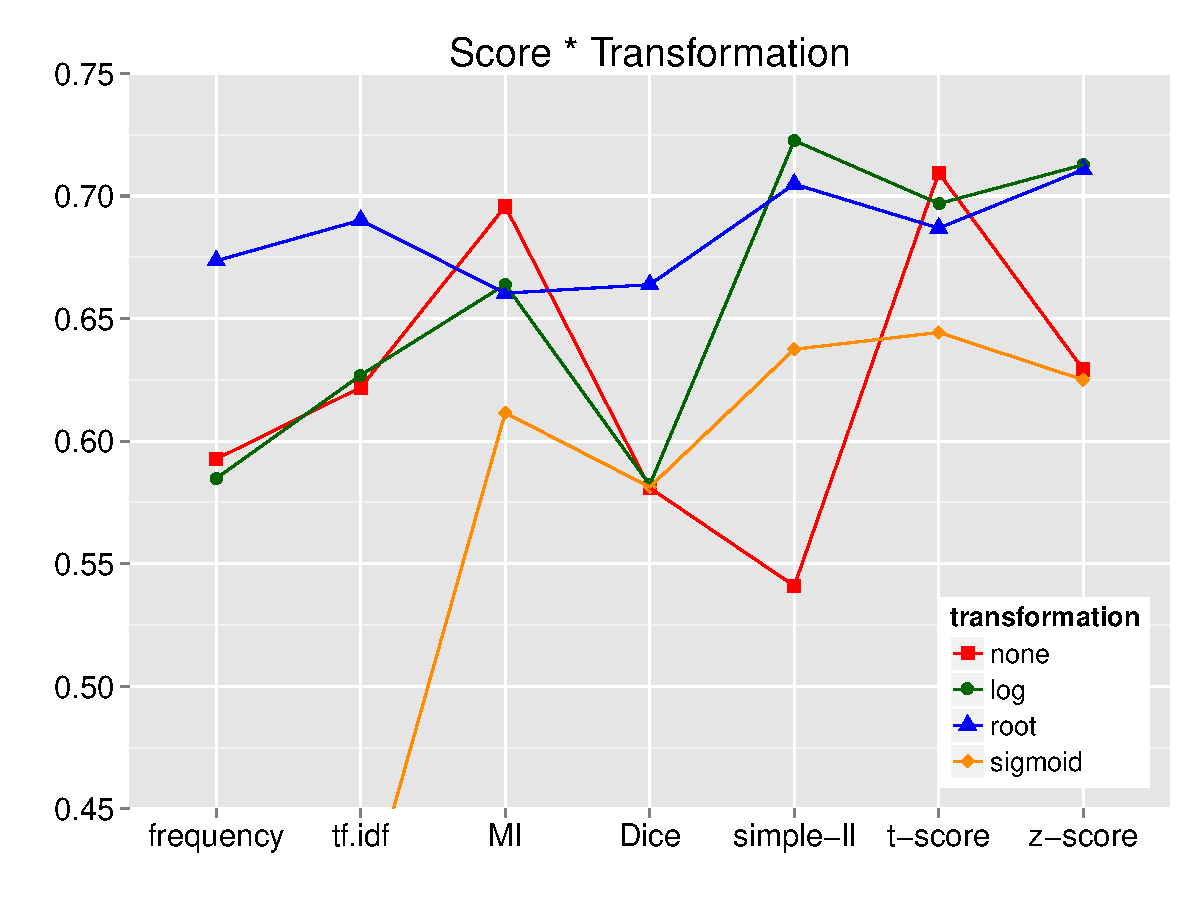
\includegraphics[scale=0.30]{img/lapesa_rg_main_score_transformation} &
    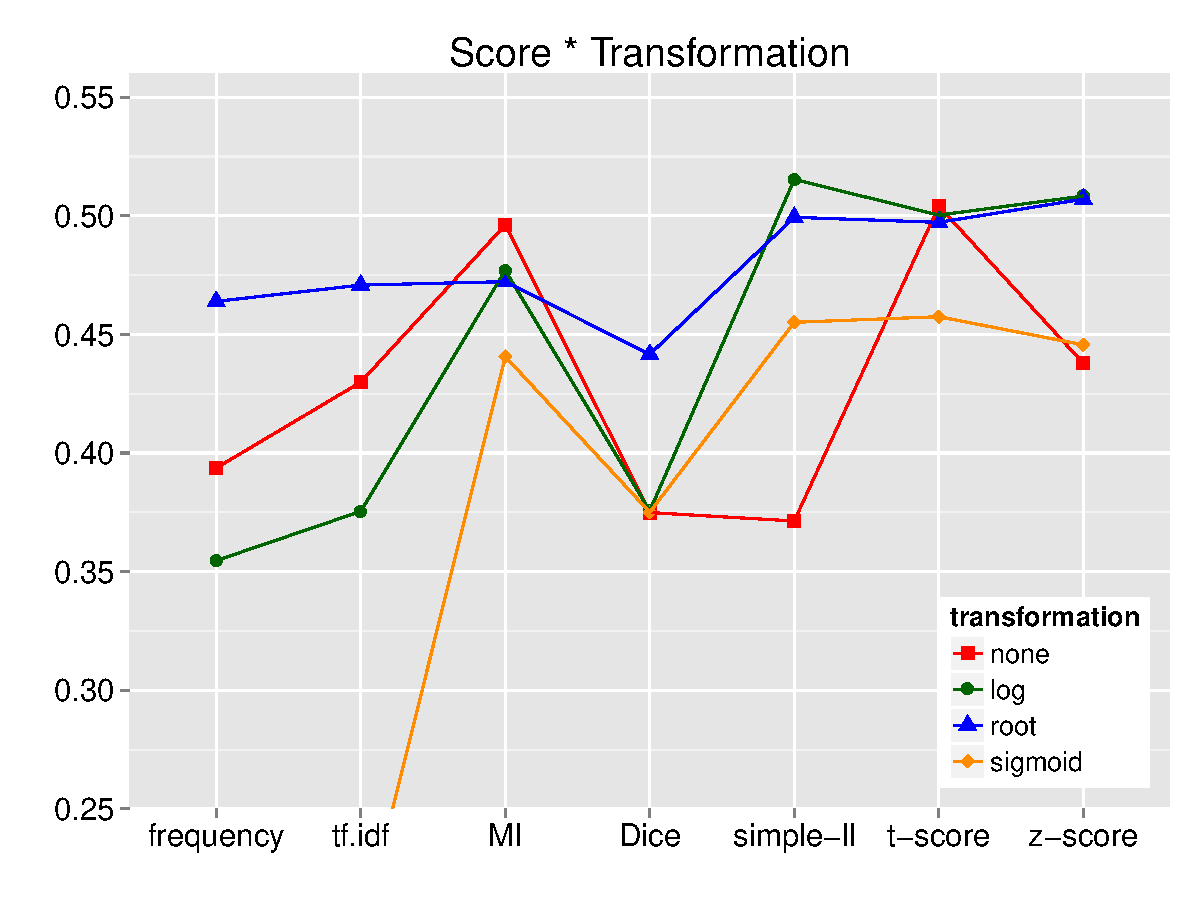
\includegraphics[scale=0.30]{img/lapesa_ws_main_score_transformation} \\
    \secondary{Rubenstein \& Goodenough} &
    \secondary{WordSim-353}
  \end{tabular}
\end{frame}


\begin{frame}
  \frametitle{Similarity ratings: Relatedness Index}
  \framesubtitle{Partial effect displays \citep{Fox:03}} 

  \centering
  \gap[1]\hspace*{-1cm}%
  \begin{tabular}{c@{}c}
    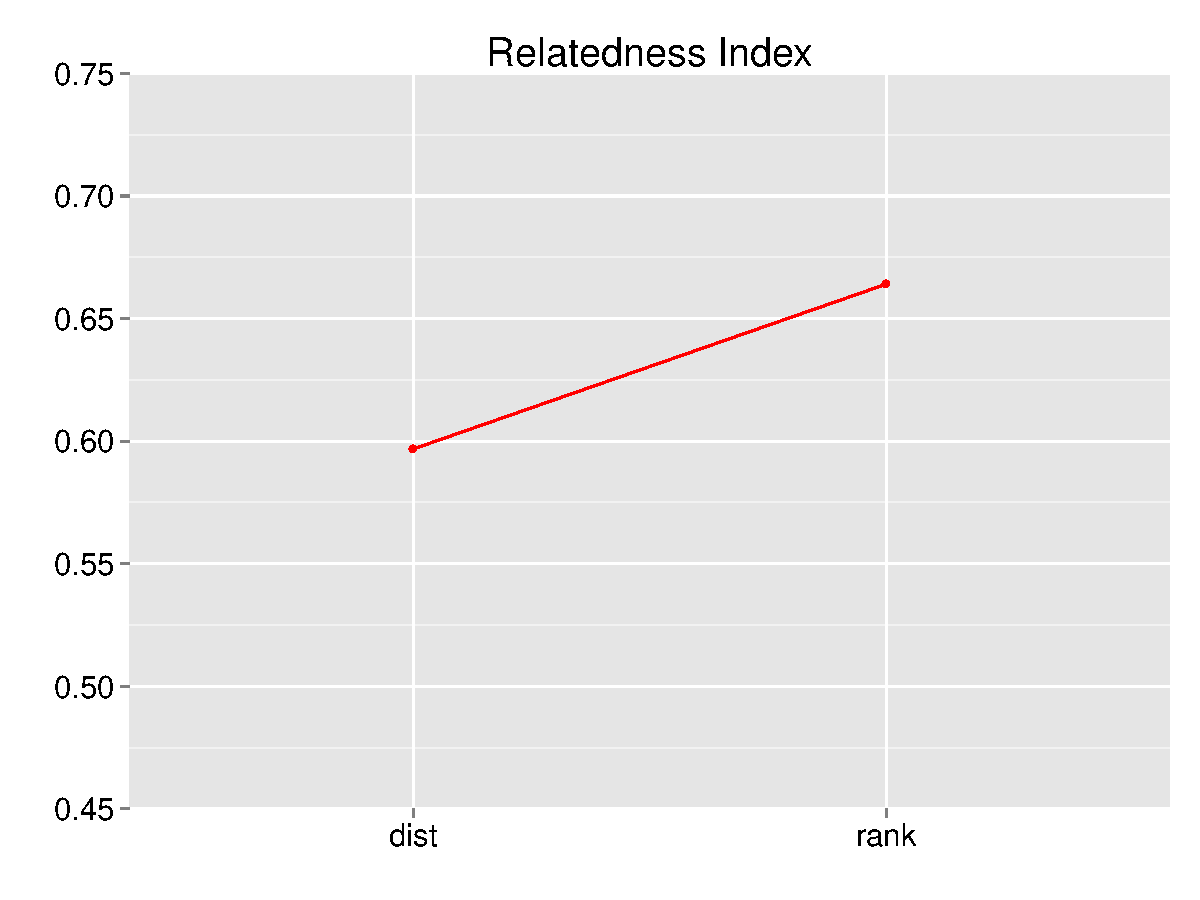
\includegraphics[scale=0.30]{img/lapesa_rg_main_relindex} &
    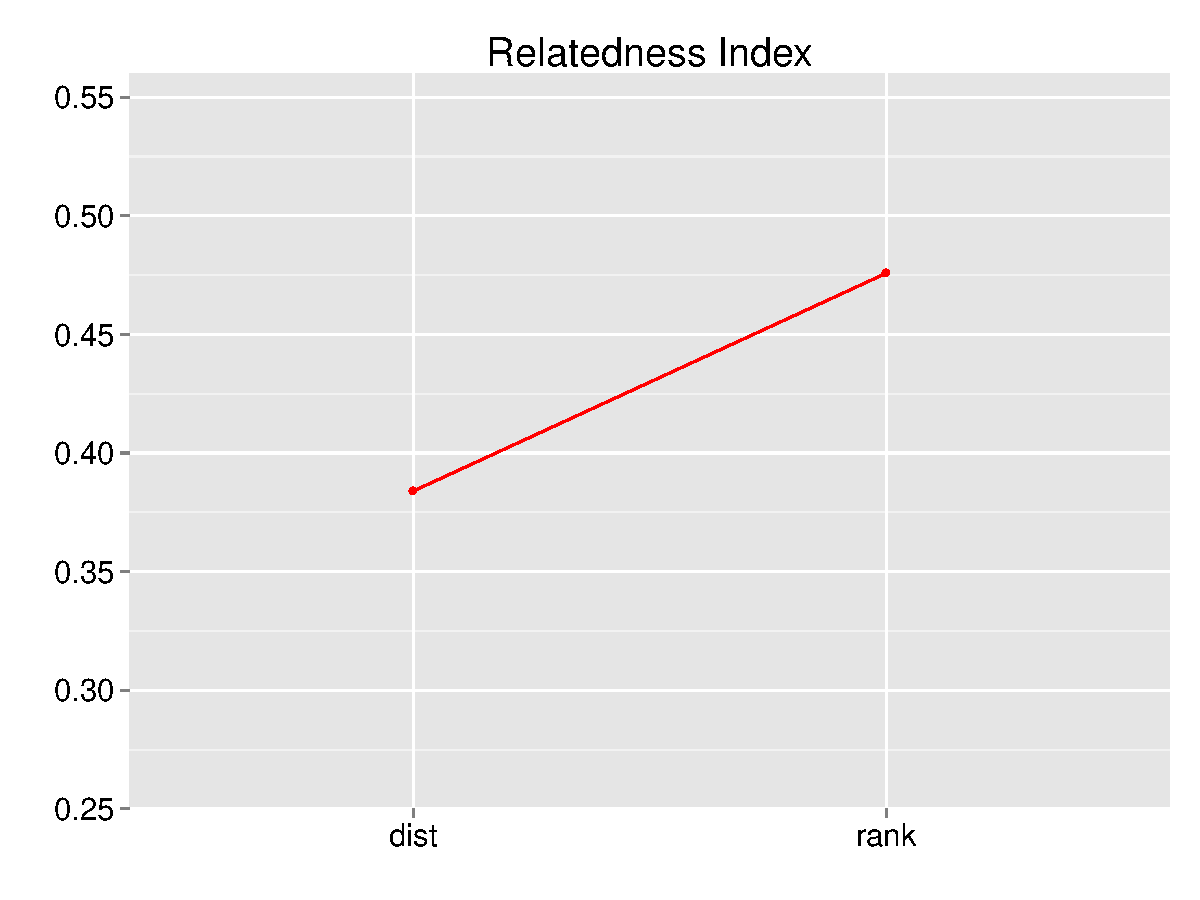
\includegraphics[scale=0.30]{img/lapesa_ws_main_relindex} \\
    \secondary{Rubenstein \& Goodenough} &
    \secondary{WordSim-353}
  \end{tabular}
\end{frame}

\begin{frame}
  \frametitle{Similarity ratings: Metric, Number of Feature Dimensions}
  \framesubtitle{Partial effect displays \citep{Fox:03}} 

  \centering
  \gap[1]\hspace*{-1cm}%
  \begin{tabular}{c@{}c}
    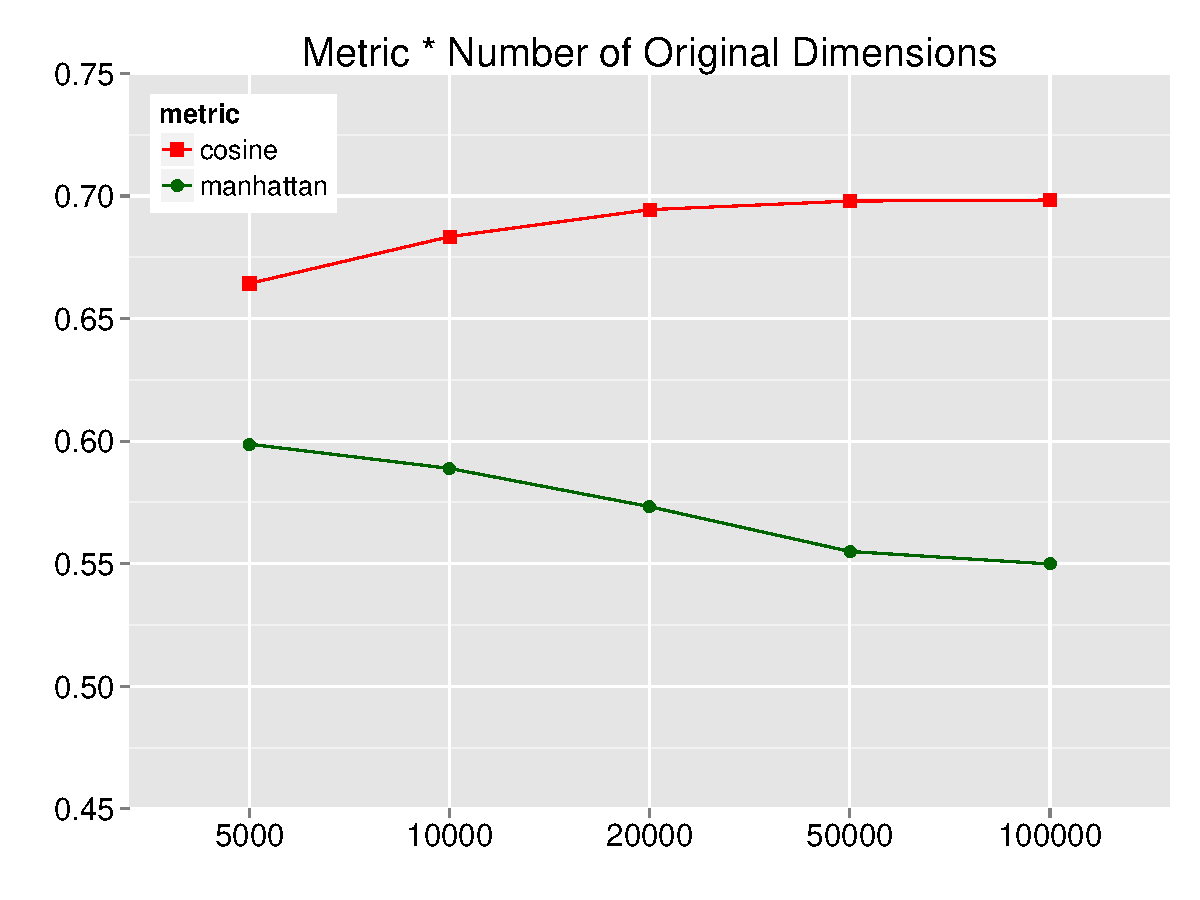
\includegraphics[scale=0.30]{img/lapesa_rg_main_metric_origdim} &
    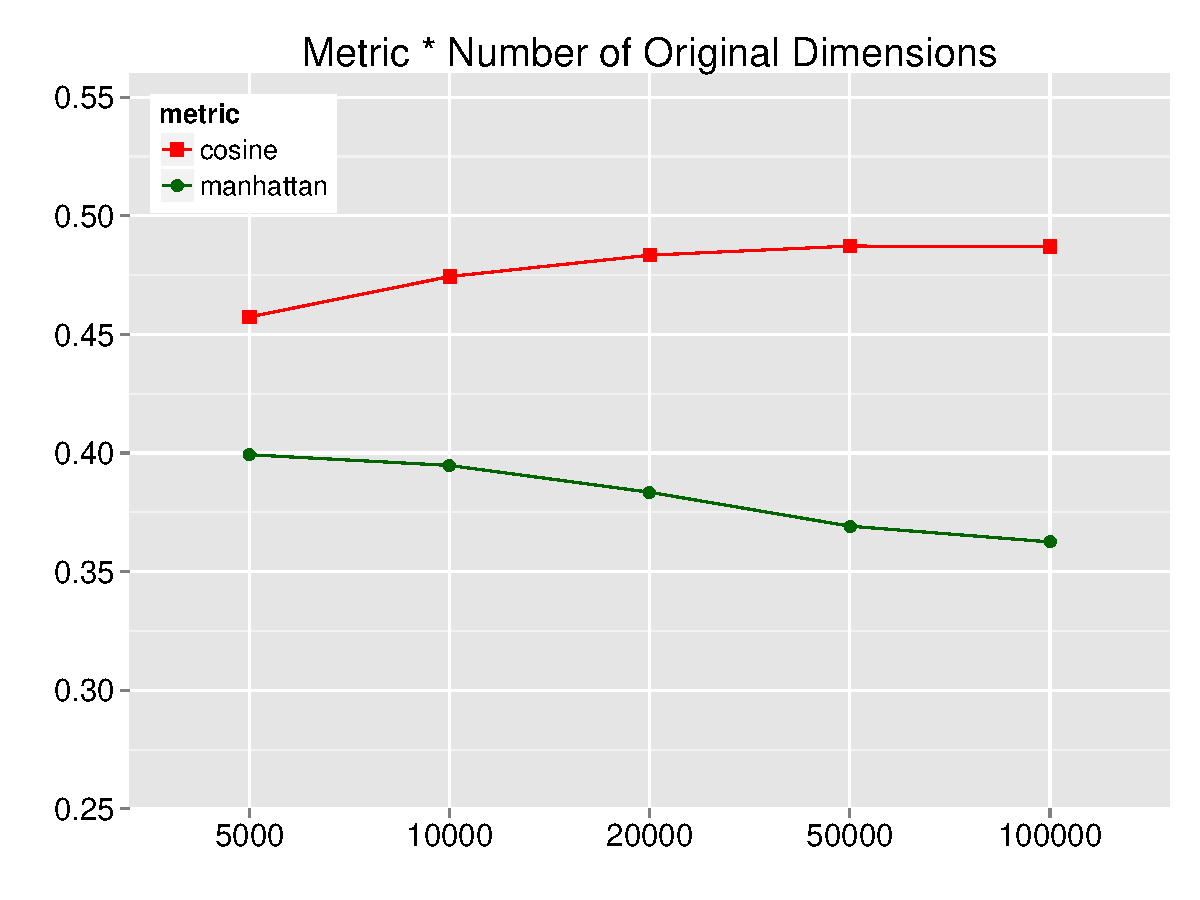
\includegraphics[scale=0.30]{img/lapesa_ws_main_metric_origdim} \\
    \secondary{Rubenstein \& Goodenough} &
    \secondary{WordSim-353}
  \end{tabular}
\end{frame}

\begin{frame}
  \frametitle{Similarity ratings: Number of Latent Dimensions}
  \framesubtitle{Partial effect displays \citep{Fox:03}} 

  \centering
  \gap[1]\hspace*{-1cm}%
  \begin{tabular}{c@{}c}
    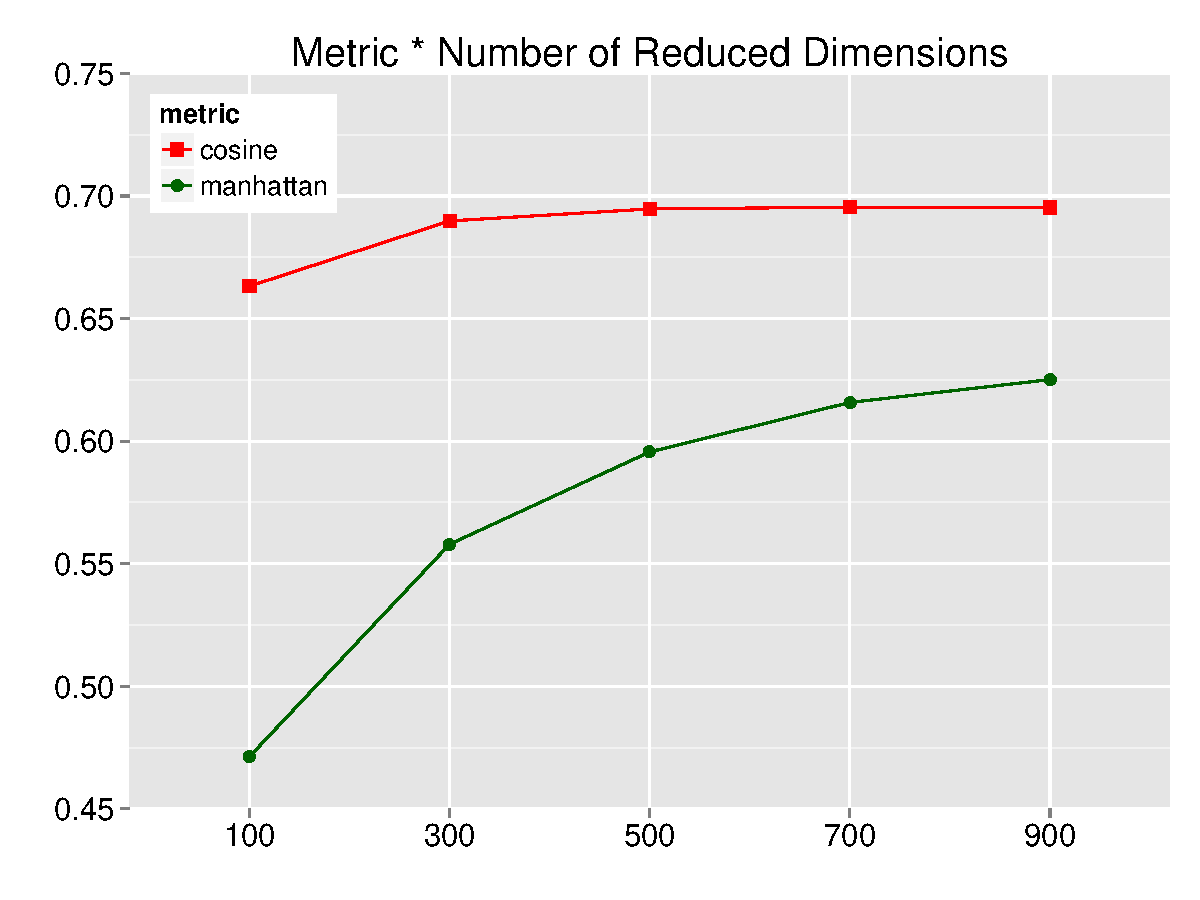
\includegraphics[scale=0.30]{img/lapesa_rg_main_metric_n-dim} &
    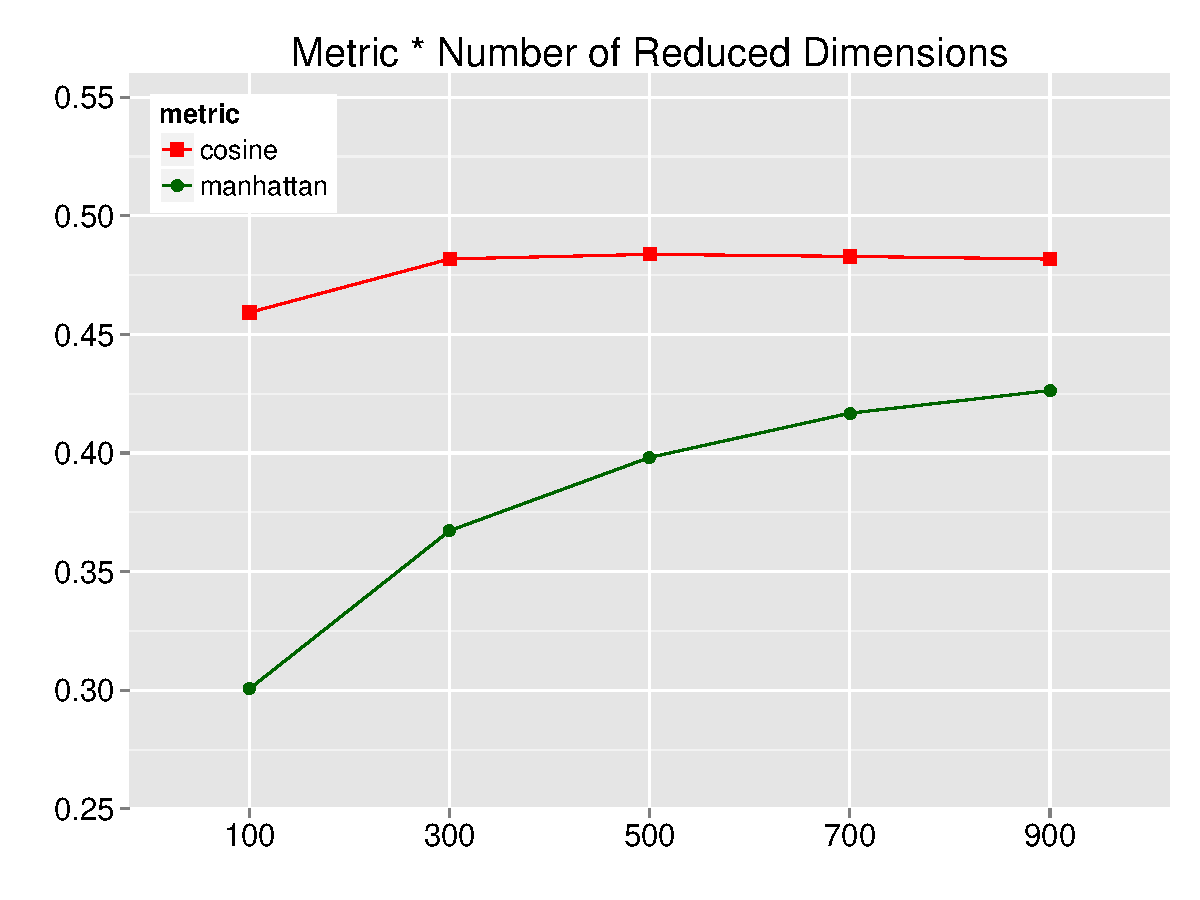
\includegraphics[scale=0.30]{img/lapesa_ws_main_metric_n-dim} \\
    \secondary{Rubenstein \& Goodenough} &
    \secondary{WordSim-353}
  \end{tabular}
\end{frame}

\begin{frame}
  \frametitle{Similarity ratings: Number of Skipped Dimensions}
  \framesubtitle{Partial effect displays \citep{Fox:03}} 

  \centering
  \gap[1]\hspace*{-1cm}%
  \begin{tabular}{c@{}c}
    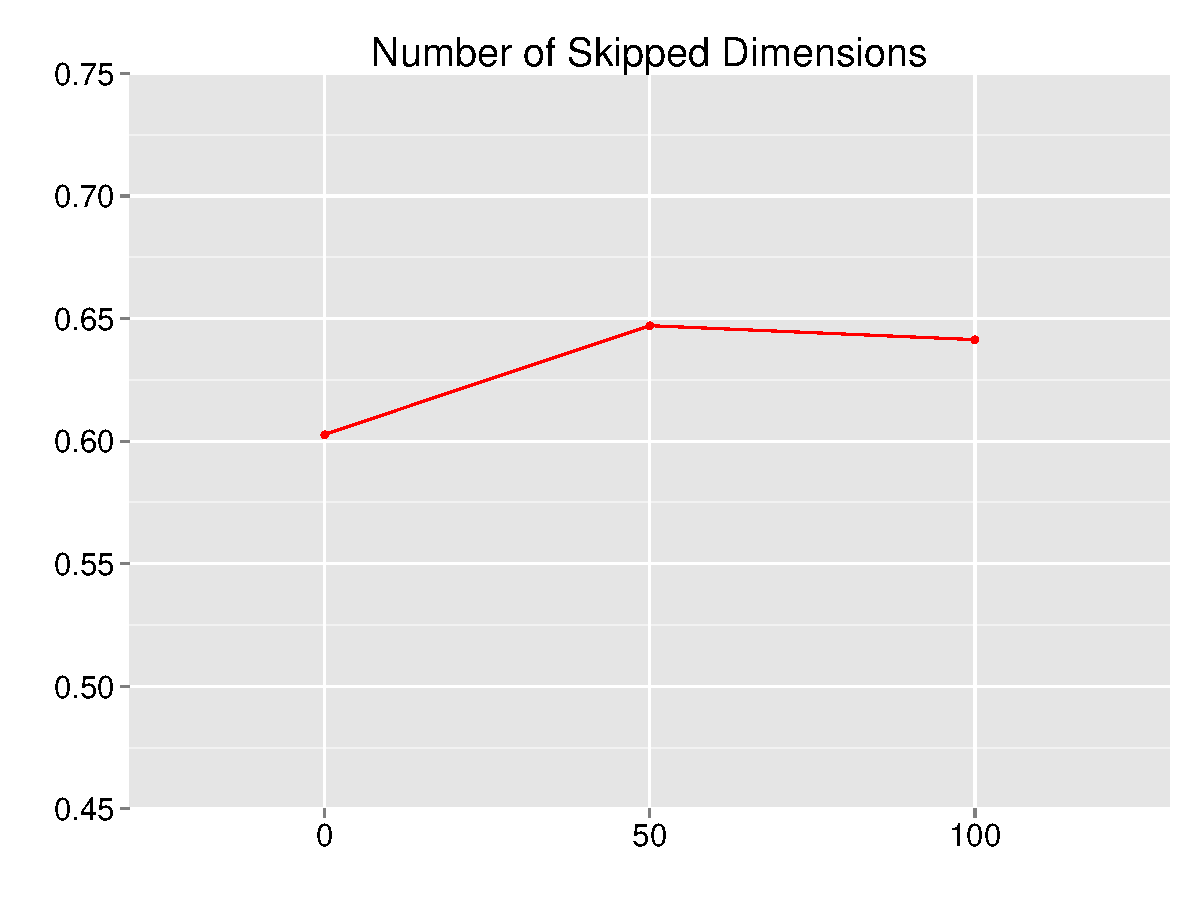
\includegraphics[scale=0.30]{img/lapesa_rg_main_dimskip} &
    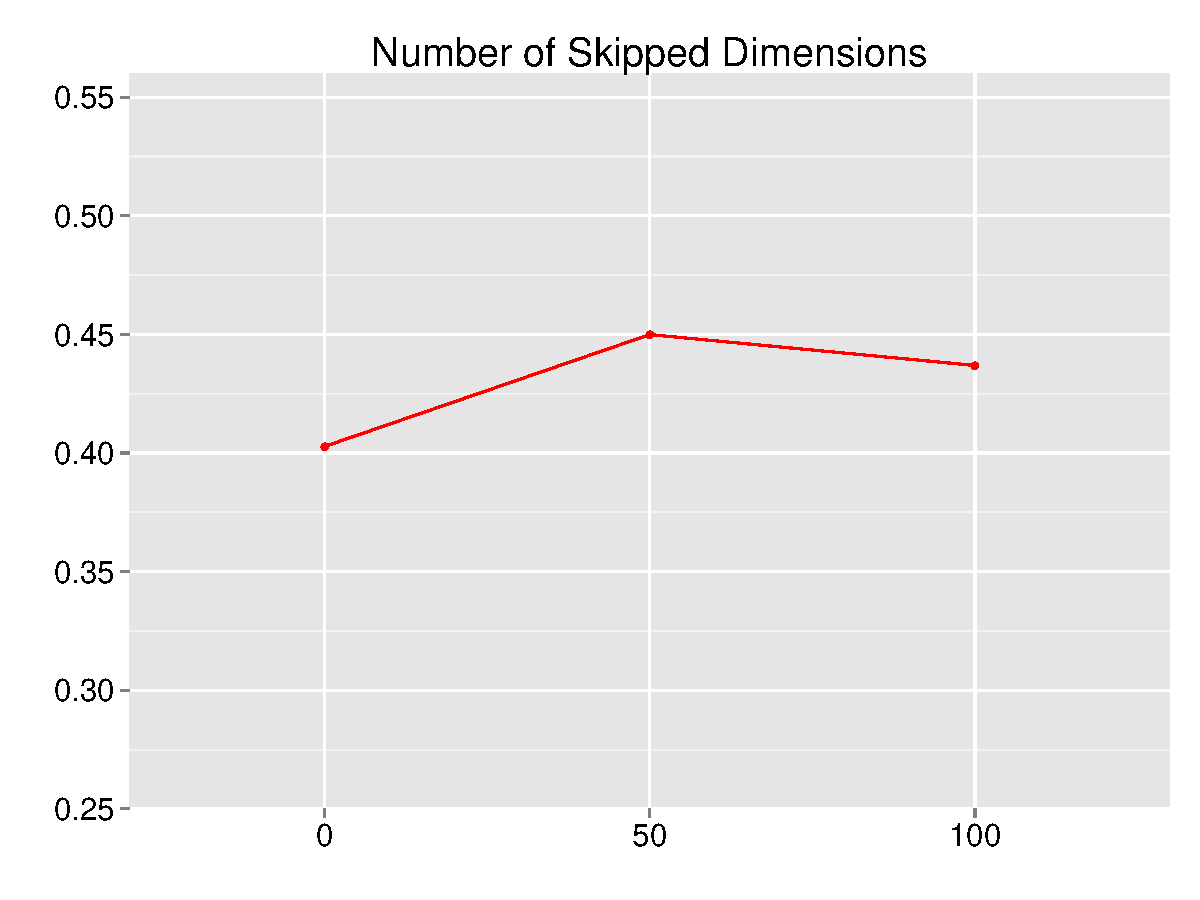
\includegraphics[scale=0.30]{img/lapesa_ws_main_dimskip} \\
    \secondary{Rubenstein \& Goodenough} &
    \secondary{WordSim-353}
  \end{tabular}
\end{frame}

\begin{frame}
  \frametitle{Similarity ratings: Window Size, Transformation}
  \framesubtitle{Partial effect displays \citep{Fox:03}} 

  \centering
  \gap[1]\hspace*{-1cm}%
  \begin{tabular}{c@{}c}
    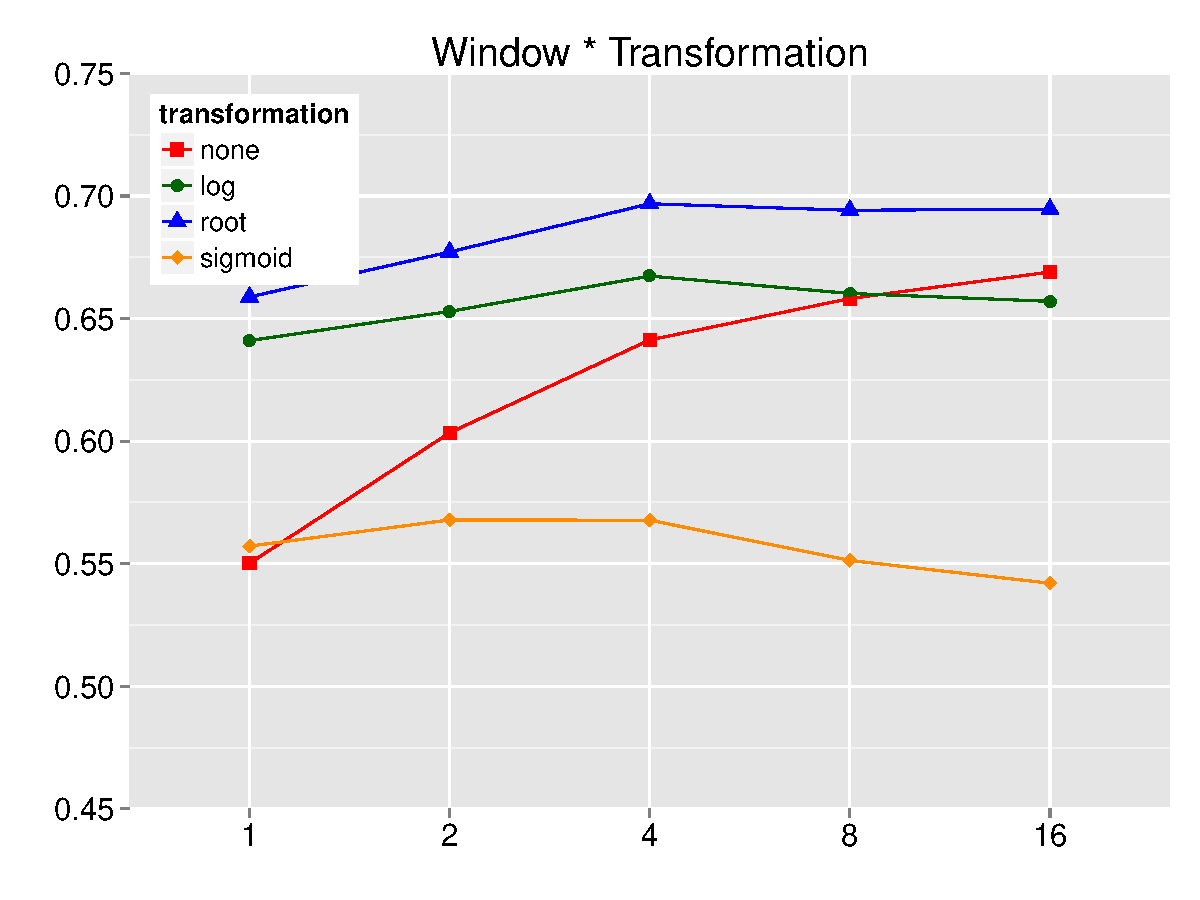
\includegraphics[scale=0.30]{img/lapesa_rg_main_window_transformation} &
    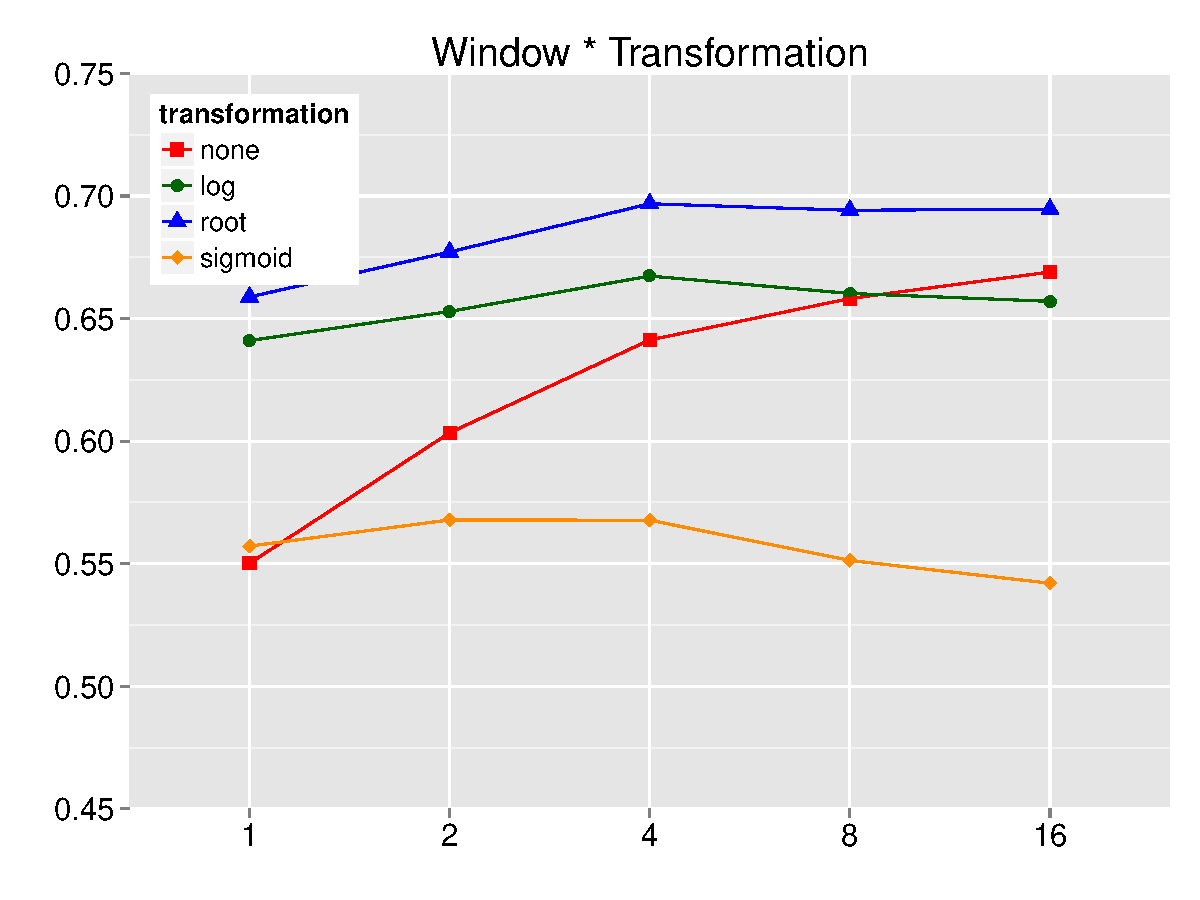
\includegraphics[scale=0.30]{img/lapesa_rg_main_window_transformation} \\
    \secondary{Rubenstein \& Goodenough} &
    \secondary{WordSim-353}
  \end{tabular}
\end{frame}

\begin{frame}
  \frametitle{Summing up: Ratings}
  \begin{exampleblock}{Ratings: best setting}
    \begin{itemize}\footnotesize
    \item Corpus: wacky
    \item Window: undirected, 4 words 
    \item Feature selection: top 20000/50000 dimensions, based on frequency
    \item Score * Transformation: simple-ll * log
    \item Dimensionality Reduction: 300 latent dimensions, skipping the first 50
    \item Distance Metric: cosine
    \item Index of Distributional Relatedness: neighbor rank
    \end{itemize}
  \end{exampleblock}  
\end{frame}


\begin{frame}
  \frametitle{DSMs and semantic clustering}
  \framesubtitle{Introducing the task}

  \ungap[1.5]
  \begin{columns}
    \begin{column}{0.5 \textwidth}
      \begin{exampleblock}{Almuhareb \& Poesio}
        \textbf{402 nouns, 21 classes} \\
        \textit{day} $\Longrightarrow$ \textsc{TIME}   \\
        \textit{kiwi} $\Longrightarrow$ \textsc{FRUIT}  \\
        \textit{kitten} $\Longrightarrow$ \textsc{ANIMAL} \\
        \textit{volleyball} $\Longrightarrow$ \textsc{GAME}
      \end{exampleblock}
      \begin{exampleblock}{ESSLLI categorization task}
        \textbf{44 nouns, 6 classes} \\
        \textit{potato} $\Longrightarrow$ \textsc{GREEN}  \\
        \textit{hammer} $\Longrightarrow$ \textsc{TOOL}  \\
        \textit{car} $\Longrightarrow$ \textsc{VEHICLE} \\
        \textit{peacock} $\Longrightarrow$ \textsc{BIRD}     
      \end{exampleblock}
    \end{column}
    \begin{column}{0.5 \textwidth}
      \begin{exampleblock}{BATTIG set}
        \textbf{83 nouns, 10 classes} \\
        \textit{chicken} $\Longrightarrow$ \textsc{BIRD}   \\
        \textit{bear} $\Longrightarrow$ \textsc{LAND\_MAMMAL}  \\
        \textit{pot} $\Longrightarrow$ \textsc{KITCHENWARE} \\
        \textit{oak} $\Longrightarrow$ \textsc{TREE} 
      \end{exampleblock}
      \begin{exampleblock}{MITCHELL set}
        \textbf{60 nouns, 12 classes} \\
        \textit{ant} $\Longrightarrow$ \textsc{INSECT}   \\
        \textit{carrot} $\Longrightarrow$ \textsc{VEGETABLE}  \\
        \textit{train} $\Longrightarrow$ \textsc{VEHICLE} \\
        \textit{cat} $\Longrightarrow$ \textsc{ANIMAL}
      \end{exampleblock}
    \end{column}
  \end{columns}
\end{frame}

\begin{frame}
  \frametitle{DSMs and semantic clustering}
  \framesubtitle{Introducing the task}

  \begin{itemize}
  \item A \textbf{categorization} task
  \item If distributional representations approximate human conceptual representations, we expect word categorization based on distributional features to produce concept clusters similar to those in the gold standard datasets
  \item Performance: \textbf{cluster purity}
    \begin{itemize}
    \item classification accuracy for optimal cluster labelling
    \item percentage of nouns that belong to the majority category within their cluster 
    \end{itemize}
  \item<2-> \secondary{Partitioning around medoids} \citep{Kaufman:Rousseeuw:90}
    \begin{itemize}
    \item implemented as \texttt{pam()} in R standard library
    \item direct comparison \so equal to or even better than CLUTO
    \item works with arbitrary dissimilarity matrix
    \end{itemize}
  \end{itemize}
\end{frame}


\begin{frame}
  \frametitle{Semantic clustering: performance}
  \framesubtitle{Overview: unreduced versus reduced experiments}

  \begin{center}
    \begin{tabular}{|l|c|c|c|c|c|c|}
      \hline
      \multirow{2}{*}{Dataset}  & \multicolumn{3}{c|}{Unreduced} &  \multicolumn{3}{c|}{Reduced} \\  \cline{2-7}
      & Min & Max & Mean & Min & Max & Mean \\ \hline
      
      AP & 0.15 & 0.73 & 0.56 & 0.13 & \primary{0.76} & 0.54 \\  
      BATTIG & 0.28 & \primary{0.99} & 0.77 & 0.23 & \primary{0.99} & 0.78  \\  
      ESSLLI & 0.32 & 0.93 & 0.72 & 0.32 & \primary{0.98} & 0.72  \\    
      MITCHELL & 0.26 & \primary{0.97} & 0.68 & 0.27 & \primary{0.97} & 0.69 \\    \hline
      
    \end{tabular}

    \gap[1]
    \secondary{Semantic clustering: summary of performance (purity)} 
  \end{center}
  
\end{frame}

\begin{frame}
  \frametitle{Semantic clustering: parameters and explained variance}
  \framesubtitle{Feature ablation  (model $R^{2}$ -- AP: 82\%;  BATTIG: 77\%; ESSLLI  58\%; MITCHELL 73\%)}

  \centering
  \hspace*{-10pt}
  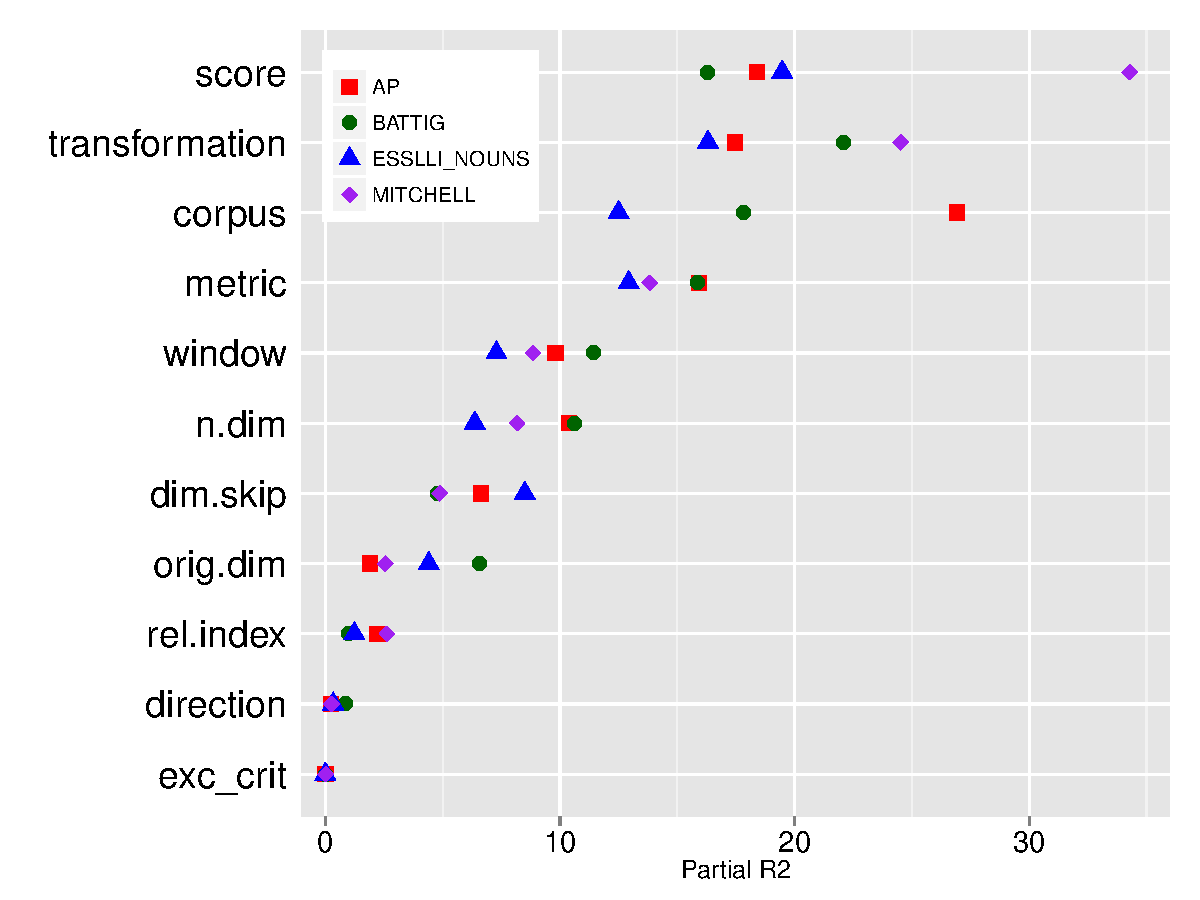
\includegraphics[scale=0.45]{img/lapesa_clustering_main_r2_reduced}
\end{frame}

\begin{frame}
  \frametitle{Semantic clustering: interactions}
  \framesubtitle{Reduced setting ($R^{2} > 0.5$)}
  
  \begin{center}\small
    \begin{tabular}{lrrrrr}
      
      Interaction & Df & AP & BATTIG & ESSLLI & MITCHELL \\ \hline
      
      \primary{score:transformation} & 18 &  7.10  & 7.95 & 7.56  &  11.42   \\ 
      \primary{window:metric} & 4 &  2.22   & 1.26 & 2.97  & 2.72    \\
      \primary{metric:n.dim} & 4 &   3.29    & 3.16 &  2.03 &  0.58   \\   
      \primary{metric:dim.skip} & 2 &   2.25   & 1.54 & 2.77  & 	 0.86  \\   
      \primary{window:transformation} & 12 &  2.00  & 2.95 & 0.88  &   2.66 \\ 


      corpus:metric & 2 &  1.42  & 2.91 & 2.79   & 1.11      \\ 
      corpus:window & 8 &   2.36   & 1.18 & 1.49  &    1.23   \\ 
      score:dim.skip & 12 &  0.56 & 1.15 &   0.99 &   1.39 \\ 
      window:score & 24 &  0.74   & 0.77 &  0.54  &  0.65  \\  
      %% metric:orig.dim & 4 &    -  & 1.20 &  0.67  &  0.92  \\ 
      %% transformation:dim.skip & 6 &   -   & 1.17 &  0.85  &  1.39    \\   
    \end{tabular}

    \gap[1]\normalsize
    \secondary{Clustering datasets: interactions, $R^2$} 
  \end{center}
  
\end{frame}

\begin{frame}
  \frametitle{Semantic clustering: Score, Transformation}
  \framesubtitle{Partial effect displays \citep{Fox:03}} 

  \centering
  \gap[1]\hspace*{-1cm}%
  \begin{tabular}{c@{}c}
    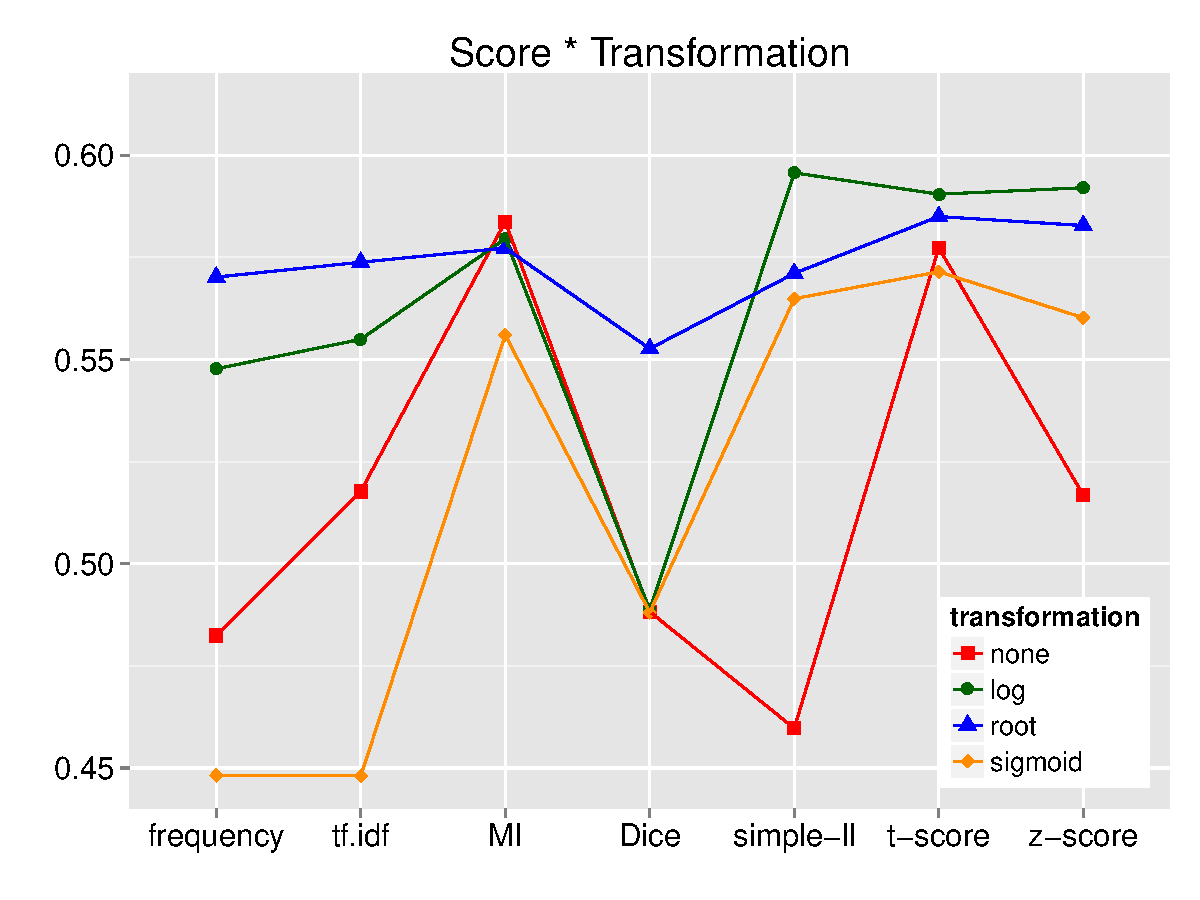
\includegraphics[scale=0.30]{img/lapesa_ap_main_score_transformation} &
    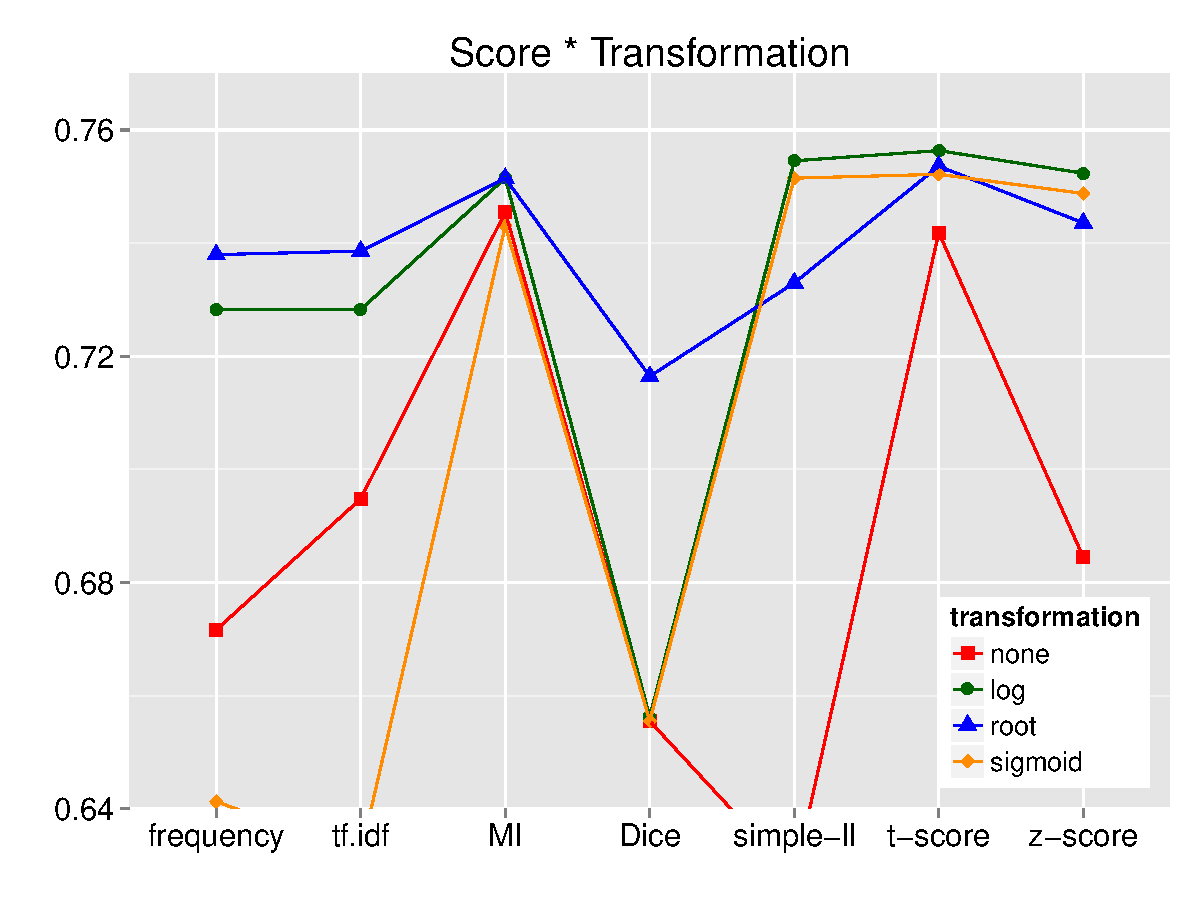
\includegraphics[scale=0.30]{img/lapesa_esslli_main_score_transformation} \\
    \secondary{Almuhareb \& Poesio} &
    \secondary{ESSLLI 2008}
  \end{tabular}
\end{frame}

\begin{frame}
  \frametitle{Semantic clustering: Corpus}
  \framesubtitle{Partial effect displays \citep{Fox:03}} 

  \centering
  \gap[1]\hspace*{-1cm}%
  \begin{tabular}{c@{}c}
    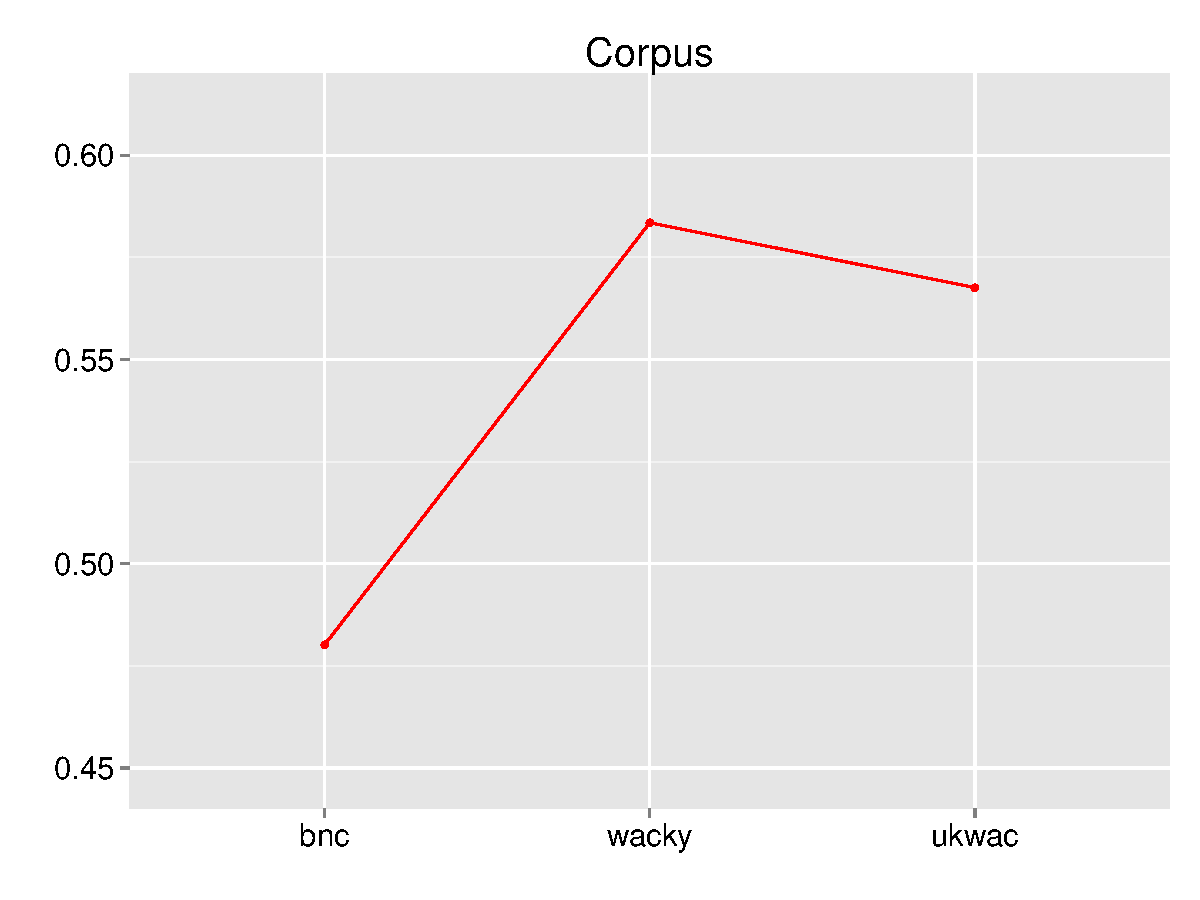
\includegraphics[scale=0.30]{img/lapesa_ap_main_corpus} &
    \includegraphics[scale=0.30]{img/lapesa_esslli_main_corpus} \\
    \secondary{Almuhareb \& Poesio} &
    \secondary{ESSLLI 2008}
  \end{tabular}
\end{frame}

\begin{frame}
  \frametitle{Semantic clustering: Window Size, Metric}
  \framesubtitle{Partial effect displays \citep{Fox:03}} 

  \centering
  \gap[1]\hspace*{-1cm}%
  \begin{tabular}{c@{}c}
    \includegraphics[scale=0.30]{img/lapesa_ap_main_window_metric} &
    \includegraphics[scale=0.30]{img/lapesa_esslli_main_window_metric} \\
    \secondary{Almuhareb \& Poesio} &
    \secondary{ESSLLI 2008}
  \end{tabular}
\end{frame}

\begin{frame}
  \frametitle{Semantic clustering: Metric, Number of Latent Dimensions}
  \framesubtitle{Partial effect displays \citep{Fox:03}} 

  \centering
  \gap[1]\hspace*{-1cm}%
  \begin{tabular}{c@{}c}
    \includegraphics[scale=0.30]{img/lapesa_ap_main_metric_n-dim} &
    \includegraphics[scale=0.30]{img/lapesa_esslli_main_metric_n-dim} \\
    \secondary{Almuhareb \& Poesio} &
    \secondary{ESSLLI 2008}
  \end{tabular}
\end{frame}

\begin{frame}
  \frametitle{Semantic clustering: Number of Skipped Dimensions}
  \framesubtitle{Partial effect displays \citep{Fox:03}} 

  \centering
  \gap[1]\hspace*{-1cm}%
  \begin{tabular}{c@{}c}
    \includegraphics[scale=0.30]{img/lapesa_ap_main_dimskip} &
    \includegraphics[scale=0.30]{img/lapesa_esslli_main_dimskip} \\
    \secondary{Almuhareb \& Poesio} &
    \secondary{ESSLLI 2008}
  \end{tabular}
\end{frame}

\begin{frame}
  \frametitle{Semantic clustering: Relatedness Index}
  \framesubtitle{Partial effect displays \citep{Fox:03}} 

  \centering
  \gap[1]\hspace*{-1cm}%
  \begin{tabular}{c@{}c}
    \includegraphics[scale=0.30]{img/lapesa_ap_main_relindex} &
    \includegraphics[scale=0.30]{img/lapesa_esslli_main_relindex} \\
    \secondary{Almuhareb \& Poesio} &
    \secondary{ESSLLI 2008}
  \end{tabular}
\end{frame}

\begin{frame}
  \frametitle{Semantic clustering: Number of Feature Dimensions}
  \framesubtitle{Partial effect displays \citep{Fox:03}} 

  \centering
  \gap[1]\hspace*{-1cm}%
  \begin{tabular}{c@{}c}
    \includegraphics[scale=0.30]{img/lapesa_ap_main_origdim} &
    \includegraphics[scale=0.30]{img/lapesa_esslli_main_origdim} \\
    \secondary{Almuhareb \& Poesio} &
    \secondary{ESSLLI 2008}
  \end{tabular}
\end{frame}

\begin{frame}
  \frametitle{Summing up: Semantic Clustering}
  \begin{exampleblock}{Clustering: best setting}
    \begin{itemize}
    \item Corpus: wacky
    \item Window: undirected, 4 words 
    \item Feature selection: top 50000 dimensions, based on frequency
    \item Score * Transformation: simple-ll * log (or t-score * log)
    \item Dimensionality Reduction: 300/500 latent dimensions,\\ no skipping necessary
    \item Distance Metric: cosine
    \item Index of Distributional Relatedness: neighbor rank
    \end{itemize}
  \end{exampleblock}   
  
\end{frame}


%%%%%%%%%%%%%%%%%%%%%%%%%%%%%%%%%%%%%%%%%%
\subsection{Summary \& conclusion}

\begin{frame}
  \frametitle{Does our evaluation methodology work?}

  \begin{enumerate}
  \item What are the most explanatory parameters?
  \item By inspecting the effect plots, we identified best settings for every dataset: what is the performance of such best settings? Are they close to the best runs in the experiment? 
  \item Is it possible to identify a general best setting that performs reasonably well across all tasks?
  \end{enumerate}
  
\end{frame}


\begin{frame}
  \frametitle{Summary: parameters}
  
  \ungap[1]
  \begin{itemize}
  \item Parameters with strong effect on DSM performance and homogeneous behavior across tasks and datasets
    \begin{itemize}
    \item score
    \item transformation
    \item distance metric
    \end{itemize}
  \item<2-> Parameters with strong effect on DSM performance, but differences across tasks
    \begin{itemize}
    \item dimensionality reduction parameters
    \item window
    \item corpus (to a lesser extent)
    \end{itemize}
  \item<3-> A less crucial parameter with homogeneous behavior
    \begin{itemize}
    \item number of context dimensions
    \end{itemize}
  \item<4-> Parameters that have no or little effect on DSM performance
    \begin{itemize}
    \item criterion for context selection
    \item direction of the context window
    \end{itemize}
  \end{itemize}
\end{frame}

\begin{frame}
  \frametitle{How about the index of distributional relatedness?}

  \begin{figure}
    \centering
    \includegraphics[scale=0.40]{img/lapesa_relindex_priming}
  \end{figure}   
  
\end{frame}

\begin{frame}
  \frametitle{Best settings and their performance}

  \begin{center}
    \setlength{\tabcolsep}{3.5pt}
    \footnotesize
    \begin{tabular}{lrlllllllllllllllll}
      \hline
      dataset & corpus & w &  o.dim & sc & tr & m  & rel.ind & n.dim & d.sk & best.s & best.m\\  \hline
      TOEFL & ukwac & \primary{2}  & 5k & s-ll & log & cos & rank  & \primary{900} & \primary{100} & 92.5 & 98.75 \\  
      WS & wacky & \primary{4} & 50k & s-ll  & log & cos & rank   & \primary{300} & \primary{50} &  0.67  & 0.73 \\ 
      RG &  wacky & \primary{4} & 50k & s-ll  & log & cos & rank   & \primary{300} & \primary{50} & 0.86  & 0.89 \\  
      AP & wacky & \primary{4} & 20k & s-ll & log & cos & rank   & \primary{300} & \primary{0} & 0.69 & 0.76 \\ 
      BATTIG & wacky & \primary{8}  & 50k & s-ll & log & cos & rank   & \primary{500} & \primary{0} & 0.98  & 0.99 \\ 
      ESSLLI & wacky & \primary{2} & 20k & t-sc & log & cos & rank   & \primary{300} & \primary{0} & \textit{0.77} & \textit{0.98} \\   
      MITCHELL & wacky & \primary{4}  & 50k & s-ll & log & cos & rank  & \primary{500} & \primary{0} & 0.88 & 0.97 \\   \hline 
    \end{tabular}

    \gap[1]
    \secondary{\normalsize Best settings for each dataset} 

    \gap[2]
    \raggedright
    \light{\small
      w = window size, o.dim = number of feature dimensions, sc = scoring function, tr = transformation, m = metric, d.sk = number of skipped dimensions, best.s = performance of best setting for this dataset,\\ best.m = performance of best run for this dataset
    }
  \end{center}
  
\end{frame}


\begin{frame}
  \frametitle{General settings}

  \ungap[1]
  \begin{center}
    \setlength{\tabcolsep}{3.5pt}
    \footnotesize
    \begin{tabular}{lrllllllllllllr}
      \hline
      task & corpus & w &  o.dim & sc & tr. & m  & rel.ind  & n.dim  & d.sk \\  
      \hline 
      TOEFL & ukwac & 2 &  5k & s-ll & log & cos & rank  & 900 & 100 \\   
      Rating & wacky & 4 & 50k & s-ll & log & cos & rank  & 300 & 50 \\  
      Clustering & wacky & 4 & 50k & s-ll & log  & cos & rank & 500 & 0 \\ 
      \primary{General} & \primary{wacky} & \primary{4} & \primary{50k} & \primary{s-ll} & \primary{log}  & \primary{cos} & \primary{rank} & \primary{500} & \primary{50} \\ 
      \hline 
    \end{tabular}

    \gap[1]
    \secondary{\normalsize General best settings} 

    \gap[2]
    \begin{tabular}{lccc>{\color{primary}}c}
      \hline
      Task & TOEFL &  RATINGS &   CLUSTERING &  GENERAL  \\  
      \hline 
      TOEFL & 92.5 & 85.0  & 75.0 & 90.0   \\  
      WS & 0.60 & 0.67 & 0.64  & 0.68 \\  
      RG & 0.85 & 0.86  & 0.84 &  0.87 \\  
      AP & 0.60 & 0.66 & 0.67 & 0.67 \\  
      BATTIG & 0.85   & 0.91 & 0.98 & 0.90  \\  
      ESSLLI & 0.70 & 0.77  & 0.80 & 0.77  \\  
      MITCHELL & 0.73 & 0.83 &  0.88 & 0.83 \\ \hline     
    \end{tabular}

    \gap[1]
    \secondary{\normalsize General best settings -- Performance}
  \end{center}
  
\end{frame}

\begin{frame}
  \frametitle{Conclusion}

  \begin{itemize}
  \item Our results show that it is possible to find a single DSM configuration that performs relatively well on every task
    \begin{itemize}
    \item[]
    \end{itemize}
  \item The most explanatory parameters show similar behavior across all tasks and datasets
    \begin{itemize}
    \item Simple-ll * Logarithmic Transformation 
    \item Cosine Distance
    \item[]
    \end{itemize}
  \item Parameters that show variation determine the amount and nature of the shared context
    \begin{itemize}
    \item Context window: 4 is a good compromise solution
    \item Dimensionality reduction: skipping the first dimensions\\ (but not too many) generally helps 
    \item Number of Feature Terms (to a lesser extent)
    \end{itemize}
  \end{itemize}
\end{frame}


\begin{frame}
  \frametitle{Conclusion}
  
  \begin{itemize}
  \item Among the source corpora, WaCkypedia appears to be a better option than UkWaC for all tasks but TOEFL
    \begin{itemize}
    \item A good trade-off between quantity and quality?
    \item[]
    \end{itemize}
  \item As an index of distributional relatedness, neighbor rank is always better than distance, even if its contribution to model performance varies across tasks
    \begin{itemize}
    \item Perhaps some tasks/datasets are less asymmetric than others? 
    \item may need to exploit directionality in a more granular way
    \end{itemize}
  \end{itemize}
\end{frame}


%%%%%%%%%%%%%%%%%%%%%%%%%%%%%%%%%%%%%%%%%%%%%%%%%%%%%%%%%%%%%%%%%%%%%% 
%% References (if any)

\frame[allowframebreaks]{
\frametitle{References}
\bibliographystyle{natbib-stefan}
\begin{scriptsize}
  \bibliography{dsm}
\end{scriptsize}
}

\end{document}
